%Title: Beamer Presentation Template
%Author: LISA
%Year: 2020

\documentclass[10pt,aspectratio=169]{beamer}
 
%
%Setting file
%

\usepackage[T1]{fontenc}
\usepackage[utf8]{inputenc}

\usepackage[english]{babel}

\usepackage{graphicx}
\graphicspath{{images/}}
\usepackage{float}
\usepackage{tikz}
\usepackage{caption}
\usepackage{subcaption}

\usetheme{default}
\usefonttheme{structurebold}


% ---------------------------------
% color definitions
\usepackage{color}
% \definecolor{LISA_BLUE}{rgb}{0.25,0.33,0.66}
\definecolor{LISA_BLUE}{cmyk}{0.99,0.88,0.29,0.18}

\setbeamercolor{normal text}{fg=LISA_BLUE}
\setbeamercolor{frametitle}{fg=LISA_BLUE}

\newcommand\insertlocation{}  % Empty by default.
\newcommand\location[1]{\renewcommand\insertlocation{#1}}

\newcommand\insertperiod{}  % Empty by default.
\newcommand\period[1]{\renewcommand\insertperiod{#1}}



\setbeamertemplate{itemize items}[circle]
\setbeamercolor{title}{fg=white}



%-----------------------------------------Title page settings-----------------------------------------%
\title{Proton-induced fusion-evaporation reactions for actinide production at IGISOL}
\subtitle{}
\author{\small A. Raggio$^{1}$, I. Moore$^{1}$, I. Pohjalainen$^{2}$, \\ E. Rey-Herme$^{3}$, J. Saren$^{1}$, M. Vandebrouck$^{3}$ and IGISOL group}
\institute{$^{1}$ Jyv\"{a}skyl\"{a} University \\
$^{2}$ GSI Helmholtzzentrum für Schwerionenforschung GmbH\\
$^{3}$ CEA, Universite Paris-Saclay}
\period{}
\date{May 26-28, 2021}
\location{Atomic Structure of Actinides \& Related Topics}


%-----------------------------------------Title page settings-----------------------------------------%


\begin{document}

{
  \usebackgroundtemplate{
\includegraphics[width=\paperwidth]{Title.pdf}}
	\begin{frame}[noframenumbering, plain]
		\titlepage
	\end{frame}
}
%----------------------------Content---------------------------------
\begin{frame}{Content}
	\begin{textblock*}{0.5\paperwidth}(0.03\paperwidth,0.2\paperheight)
		\begin{itemize}
			\item[]<1->{Physics Cases\\
			\begin{itemize}
				\item Optical spectroscopy
				\item $^{229}$Th isomeric state
				\item A test bench for collective behavior
			\end{itemize}
			}
			\vspace{0.02\textheight}
			\item[]<2->{Actinide Quest at IGISOL\\
					\begin{itemize}
						\item Production methods
						\item High-resolution spectroscopy on Plutonium
					\end{itemize}
					}
			\vspace{0.02\textheight}
			\item[]<3->{Proton-induced Fusion-evaporation\\ with actinide targets\\
					\begin{itemize}
						\item A decay spectroscopy experiment\\ with $^{232}$Th target
						\item Production Yield
						\item Combination with Penning Trap mass measurements
					\end{itemize}
					}
		\end{itemize}
	\end{textblock*}
	\begin{textblock*}{0.5\paperwidth}(0.47\paperwidth,0.2\paperheight)
		% \vspace{0.1\textheight}
		\only<1>{\includegraphics[width=\textwidth]{Full_Chart.pdf}}%
		\only<2>{\vspace{0.2\textheight}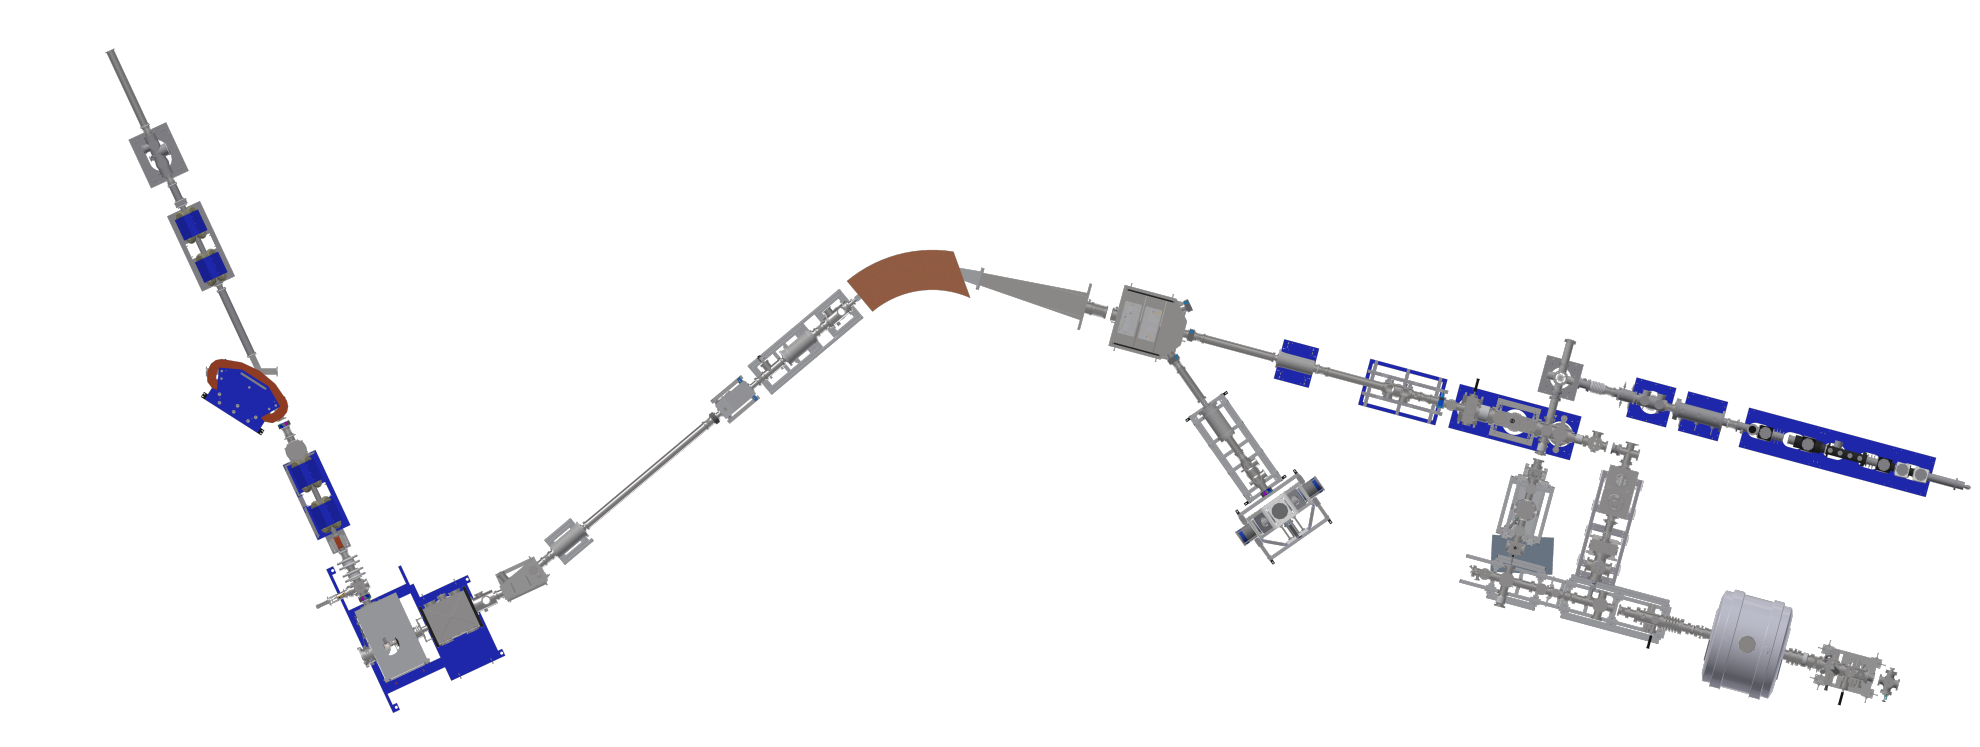
\includegraphics[width=\textwidth]{IGI-1A-IGISOL_3_no_logo.png}}%
		\only<3>{\vspace{0.2\textheight}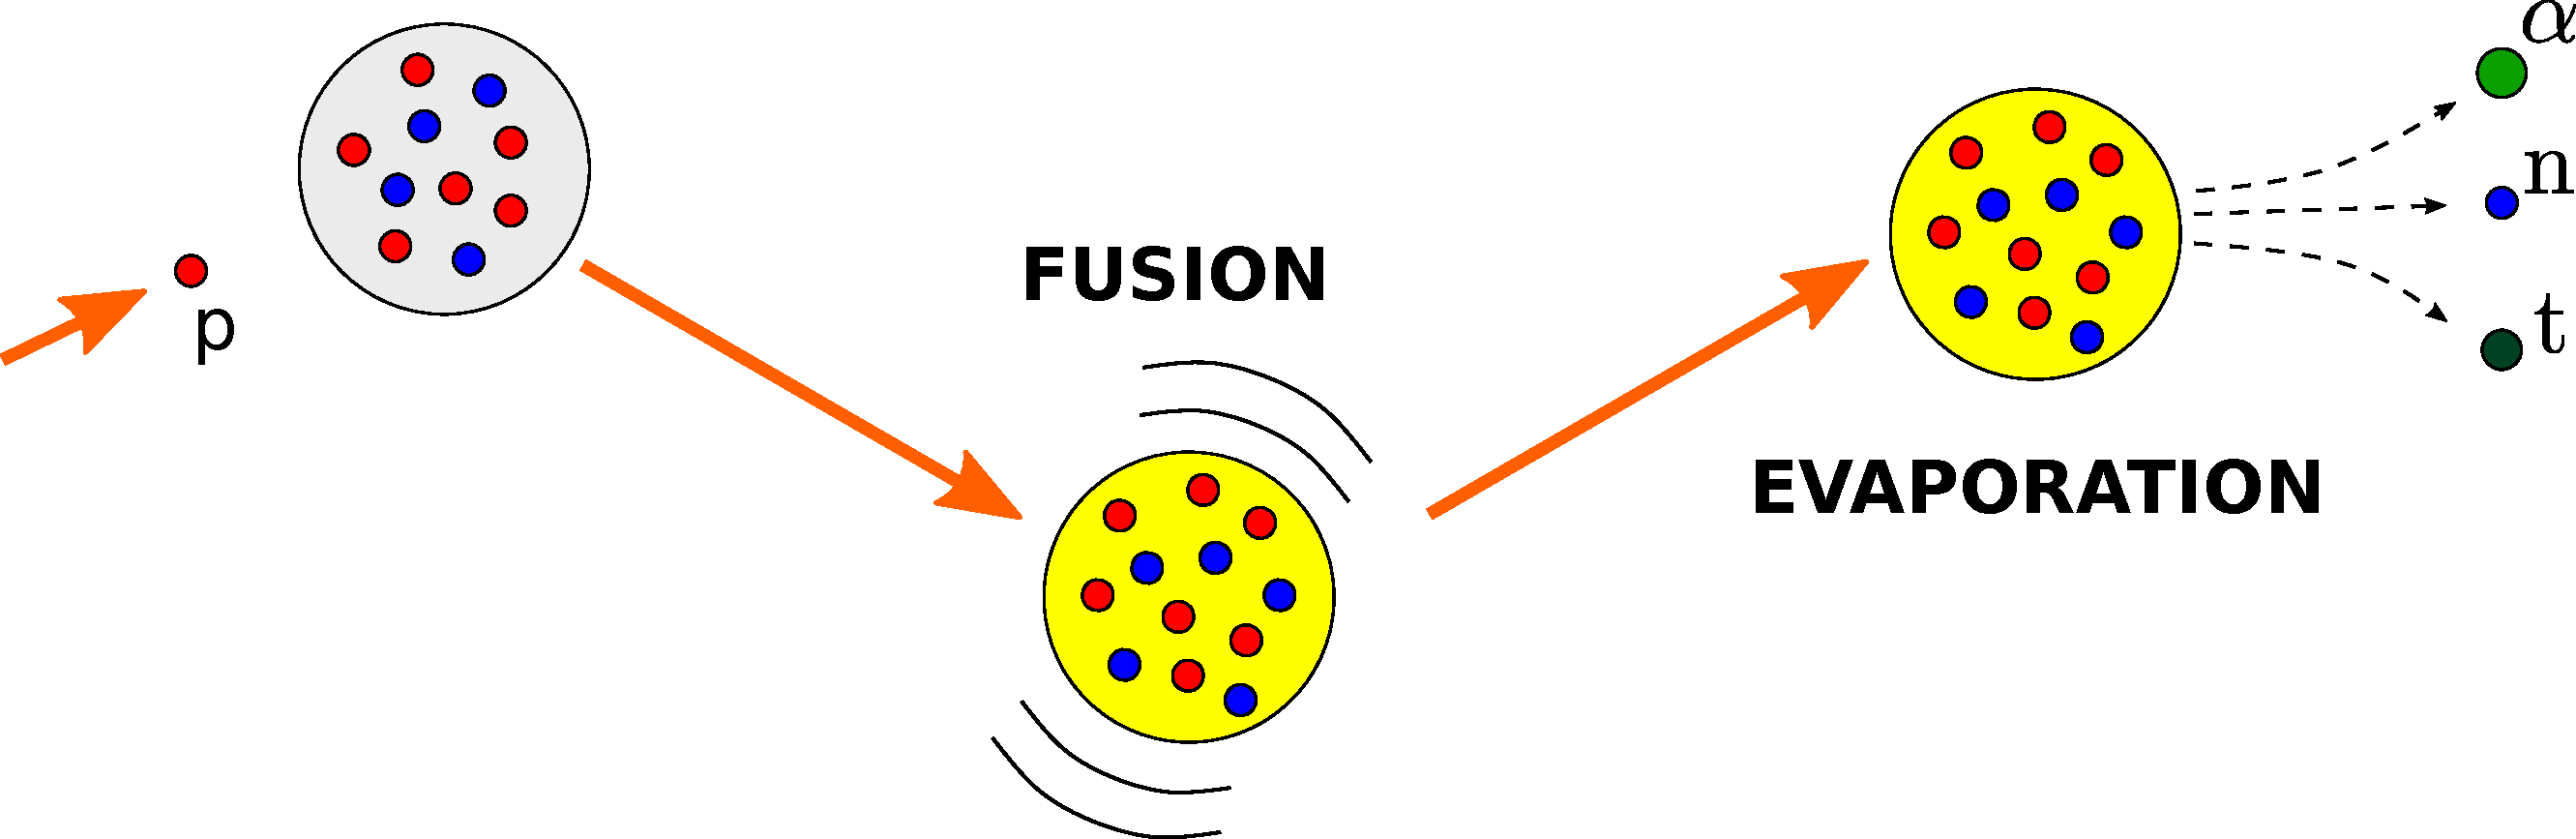
\includegraphics[width=0.9\textwidth]{Reaction.pdf}}%
	\end{textblock*}
\end{frame}

%----------------------------Motivation---------------------------------
\begin{SectionTitle}
\begin{frame}
	\centering
	\begin{textblock*}{0.5\paperwidth}(0.25\paperwidth,0.15\paperheight)
		\centering
		\textbf{\LARGE PHYSICS CASES}	
	\end{textblock*}
	\begin{textblock*}{0.5\paperwidth}(0.25\paperwidth,0.3\paperheight)
        \includegraphics[width=.8\textwidth]{Full_Chart.pdf}
	\end{textblock*}

\end{frame}
\end{SectionTitle}

\begin{frame}{Optical Spectroscopy on Actinides}
	\begin{textblock*}{0.5\paperwidth}(0.015\paperwidth,0.18\paperheight)
		\begin{textblock*}{0.1\paperwidth}(0.05\paperwidth,0.7\paperheight)
			\footnote{Updated from P. Campbell et al., PPNP 86 (2016) 127–180}
		\end{textblock*}
		\only<1>{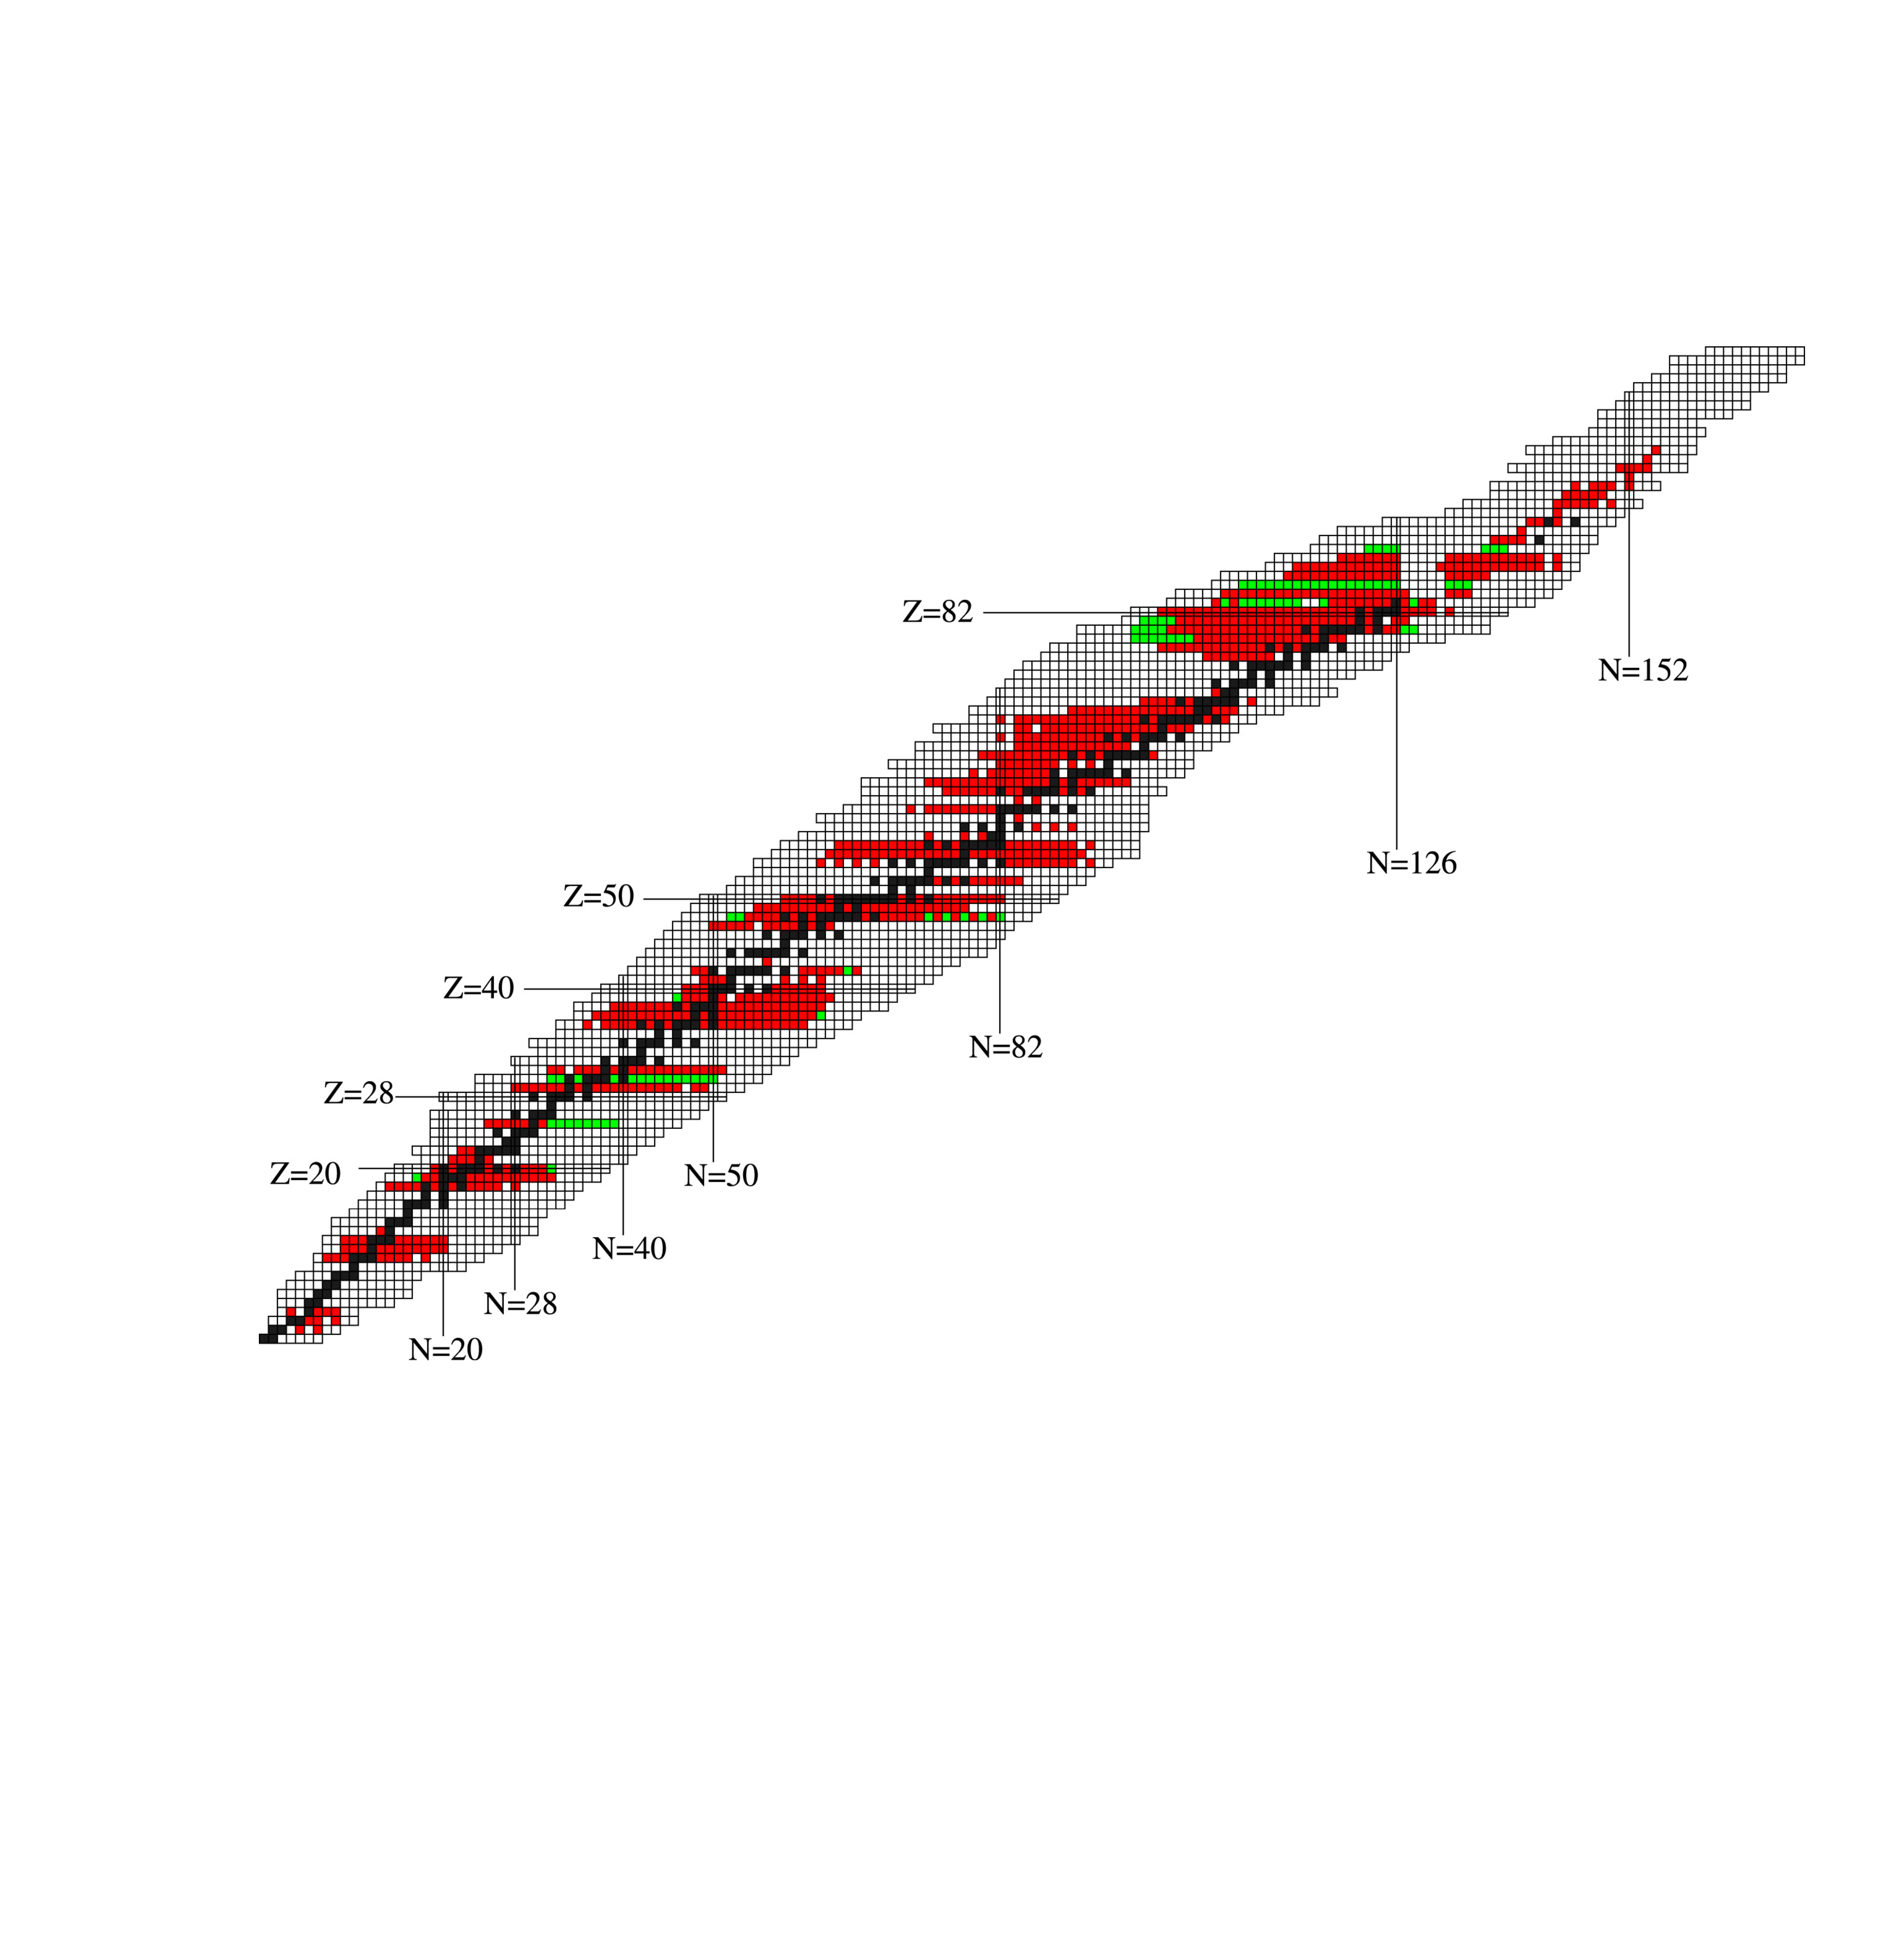
\includegraphics[width=0.8\textwidth]{AChart_0.pdf}}%
        \only<2>{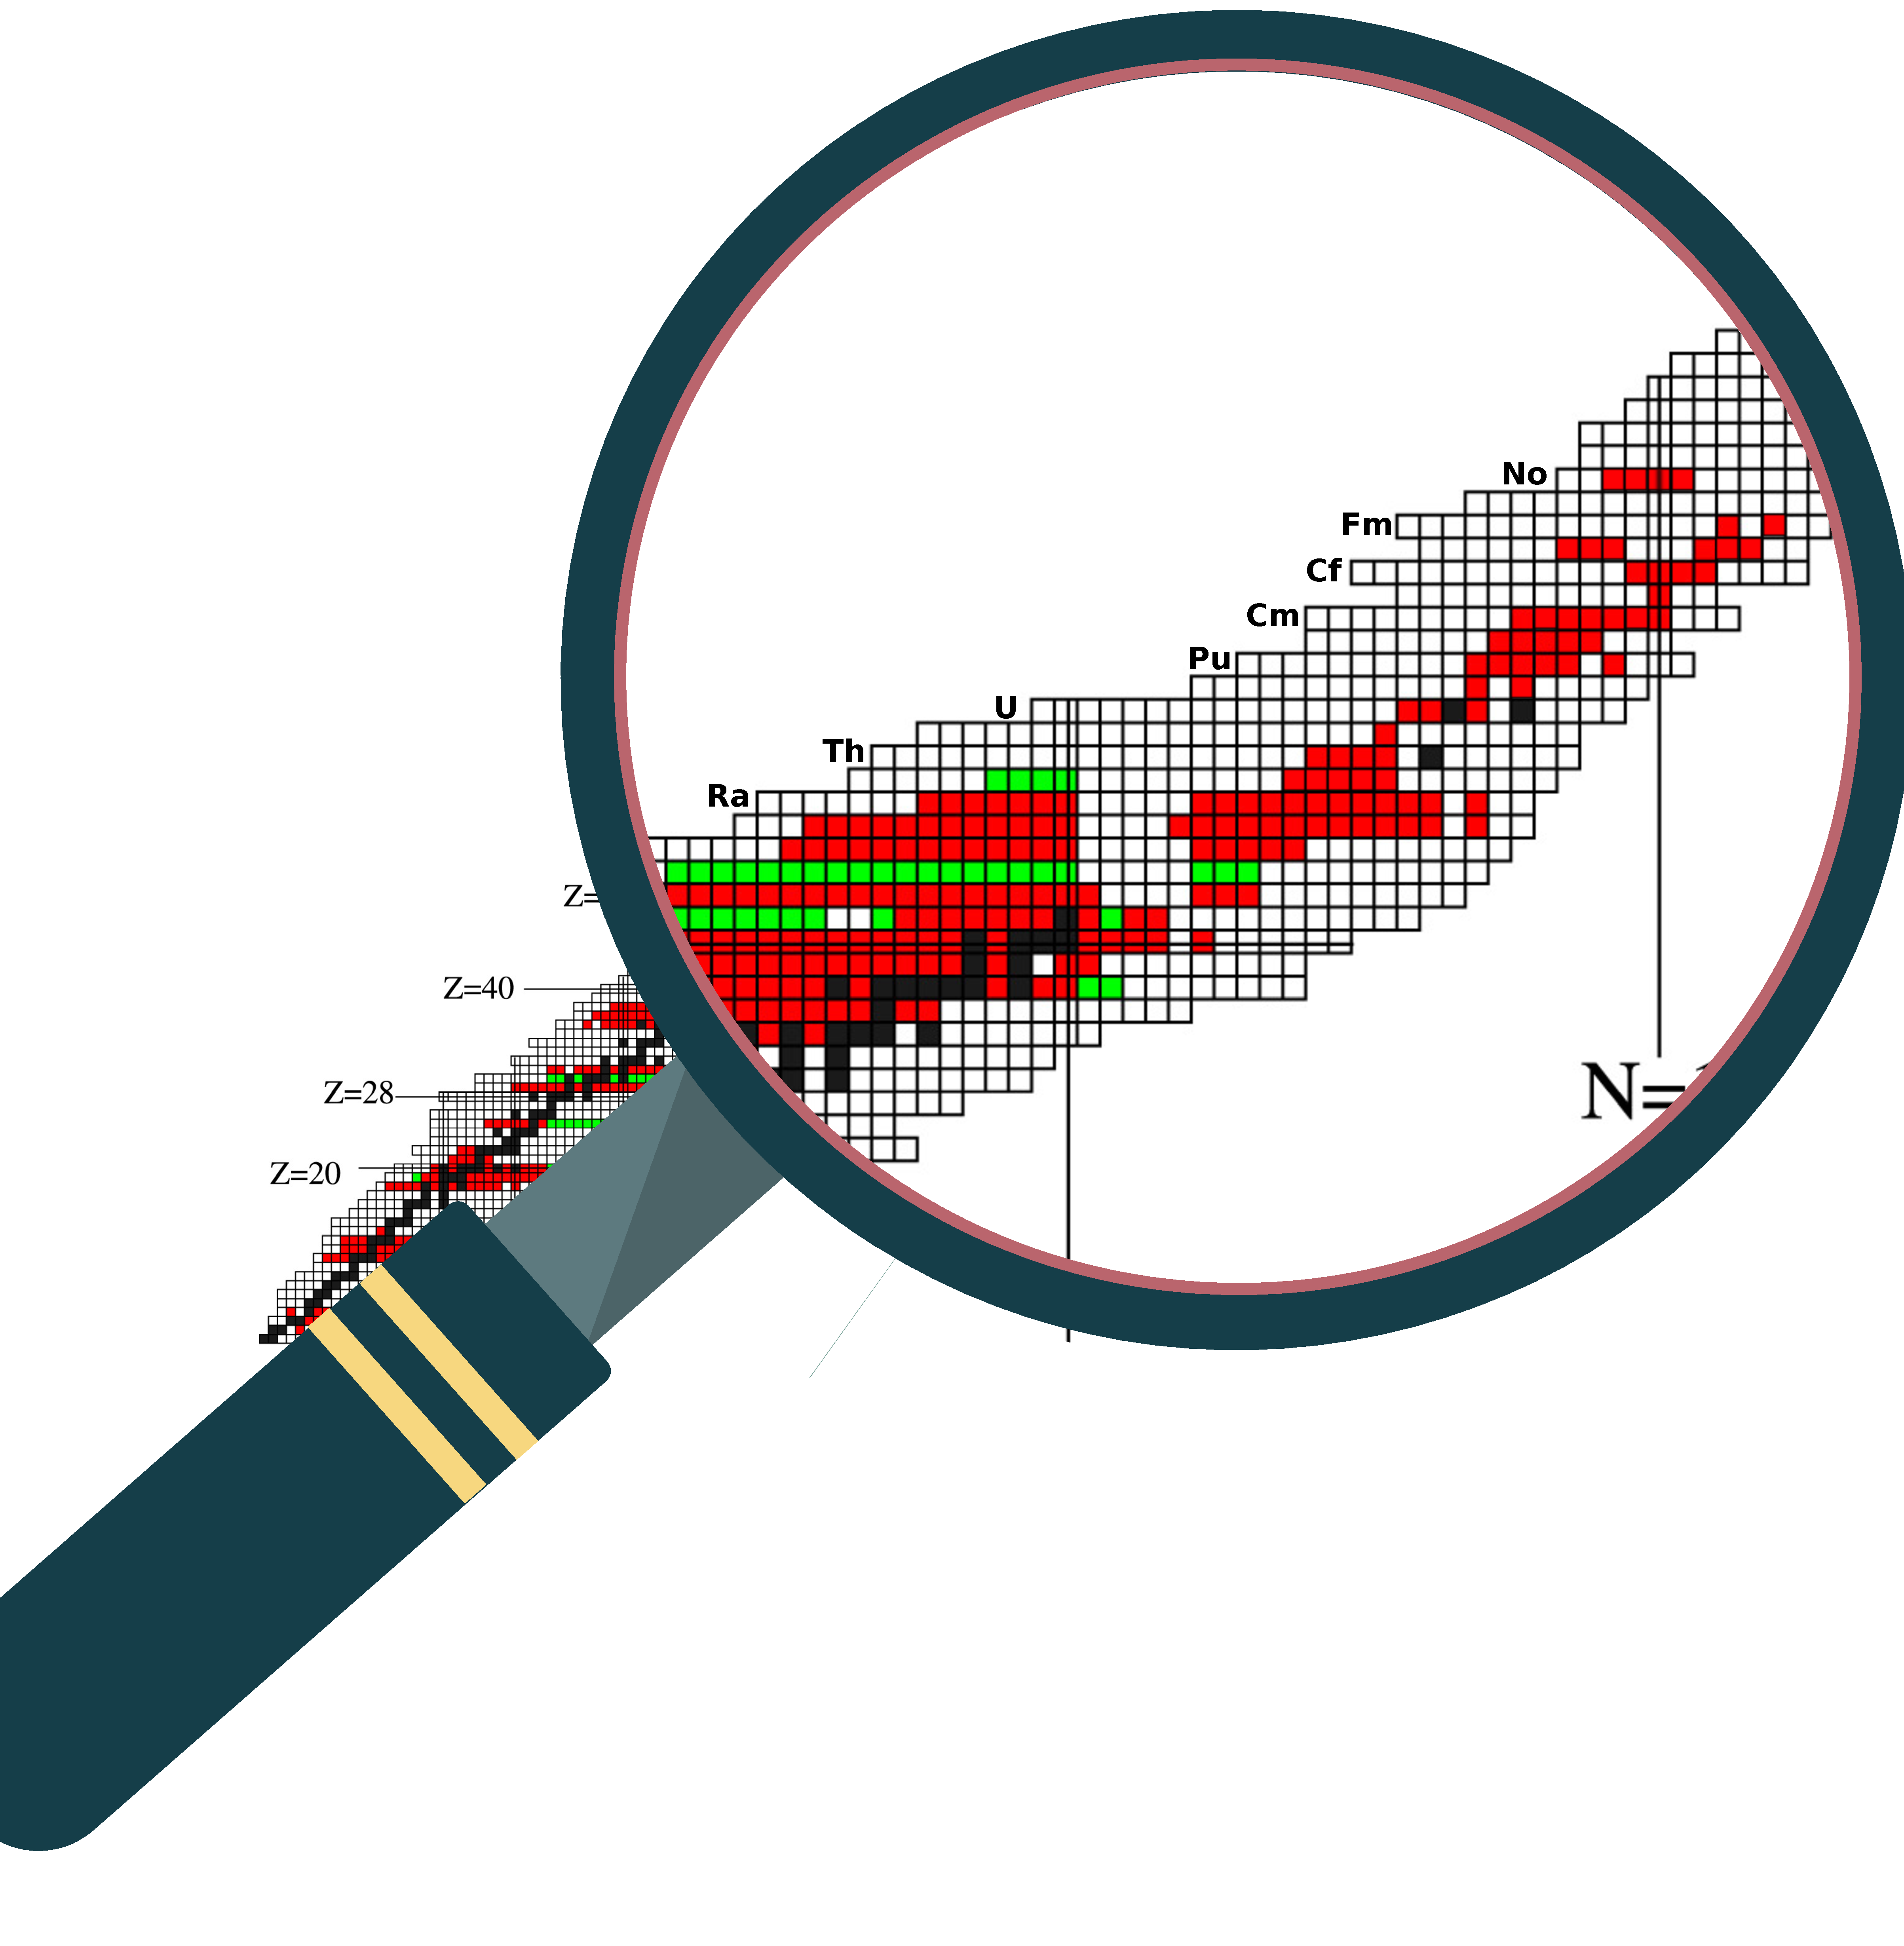
\includegraphics[width=0.8\textwidth]{AChart_1.pdf}}%
	\end{textblock*}
	\begin{textblock*}{0.6\paperwidth}(0.4\paperwidth,0.18\paperheight)
		\centering
		A useful tool to extract fundamental \\nuclear ground state properties
	\end{textblock*}
	\begin{textblock*}{0.3\paperwidth}(0.46\paperwidth,0.27\paperheight)
		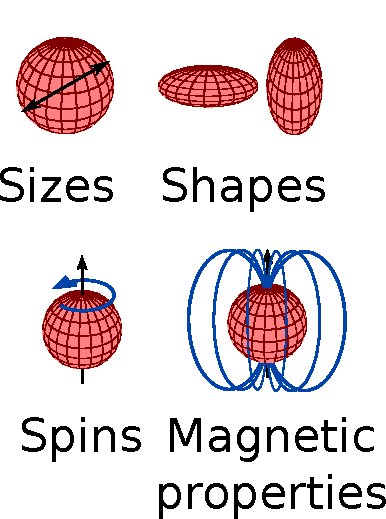
\includegraphics[width=0.5\textwidth]{shapes.pdf}
	\end{textblock*}
	\begin{textblock*}{0.5\paperwidth}(0.2\paperwidth,0.75\paperheight)
		\textbf{Nuclear model-independent measurement} 
	\end{textblock*}
	\only<2->{
	\begin{textblock*}{0.4\paperwidth}(0.65\paperwidth,0.28\paperheight)
		\textbf{General lack of optical data}
		\begin{itemize}
			\item Lack of Stable isotopes
			\item Challenging Production
		\end{itemize}
	\end{textblock*}
	\begin{textblock*}{0.4\paperwidth}(0.6\paperwidth,0.46\paperheight)
		\centering
		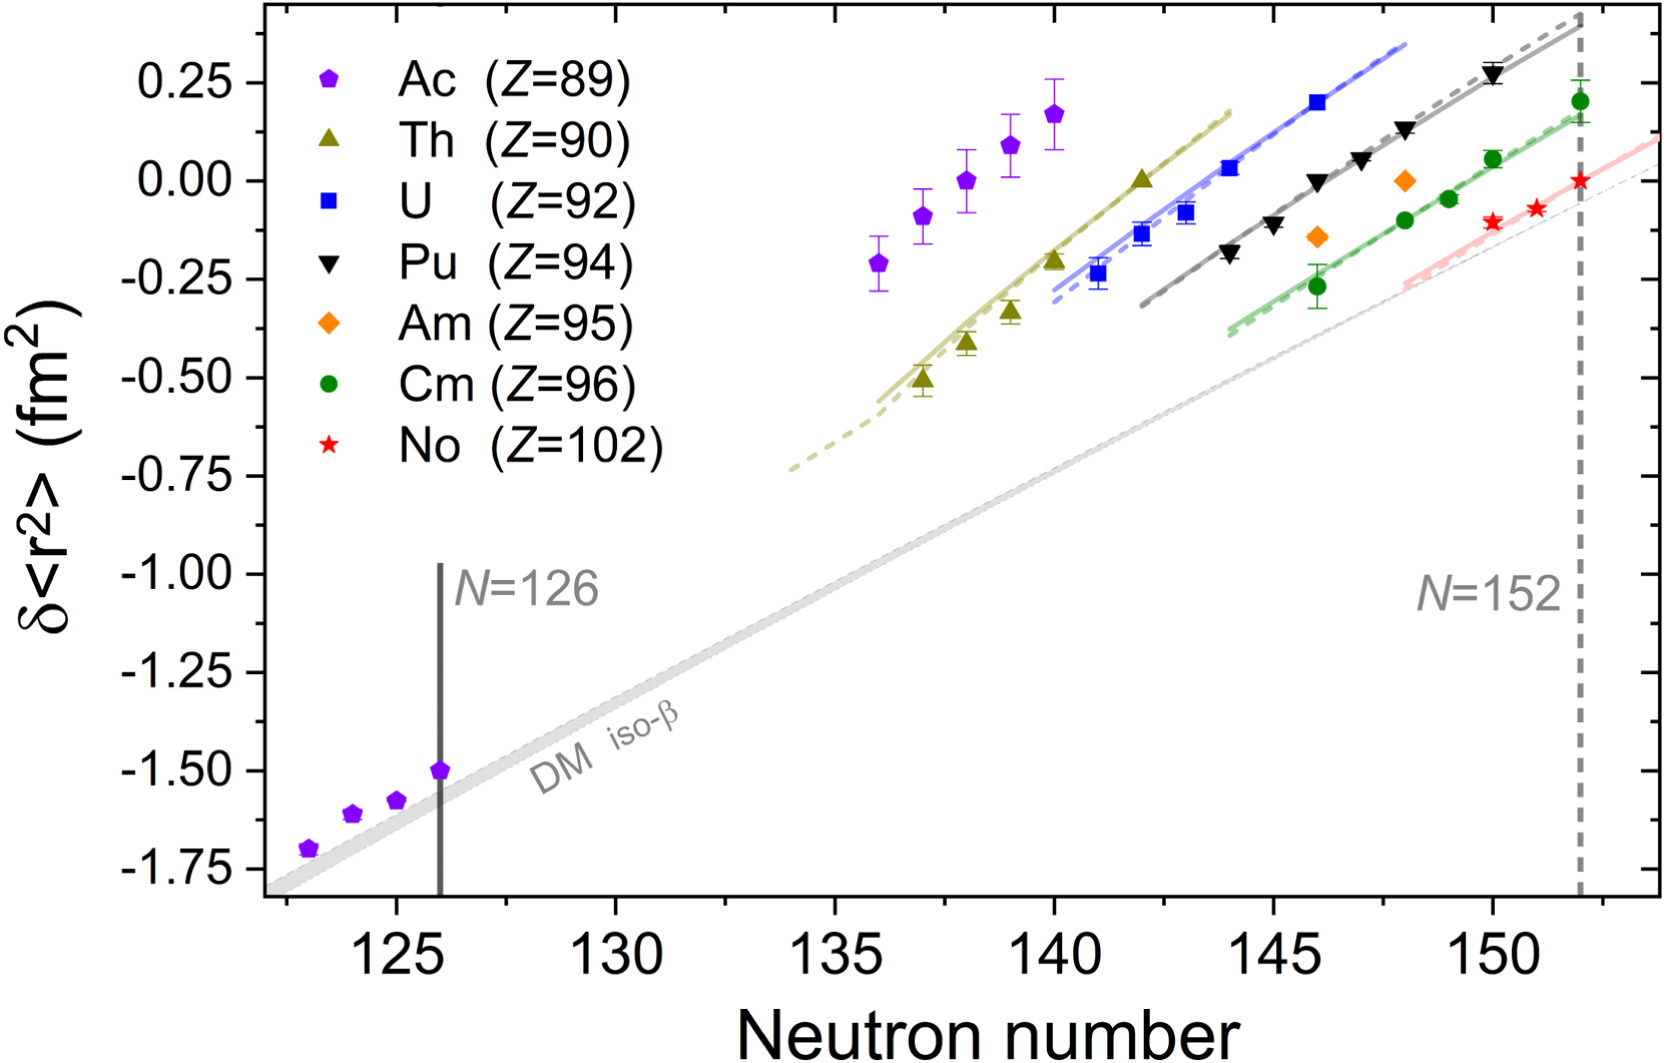
\includegraphics[width=0.8\textwidth]{MSCR.jpg}
		\footnote{M. Block et al., PPNP, 116 (2021), 103834}
	\end{textblock*}
	}
\end{frame}

\begin{frame}{Isomeric state in $^{229}$Th}
	\begin{textblock*}{0.6\paperwidth}(0.45\paperwidth,0.2\paperheight)
		% \centering
		\textbf{Measurement of the $^{229m}$Th isomer}
		\begin{itemize}
			\item HFS studied in 2$^+$ \footnote{J. Thielking, Nature 321 (2018) 556}
			\item Half-life of 1$^+$? (< 10~ms) \footnote{B. Seiferle, PRL 118.4 (2017) 042501}
			\item measurement of the 1$^+$ HFS with CLS
		\end{itemize}
		
		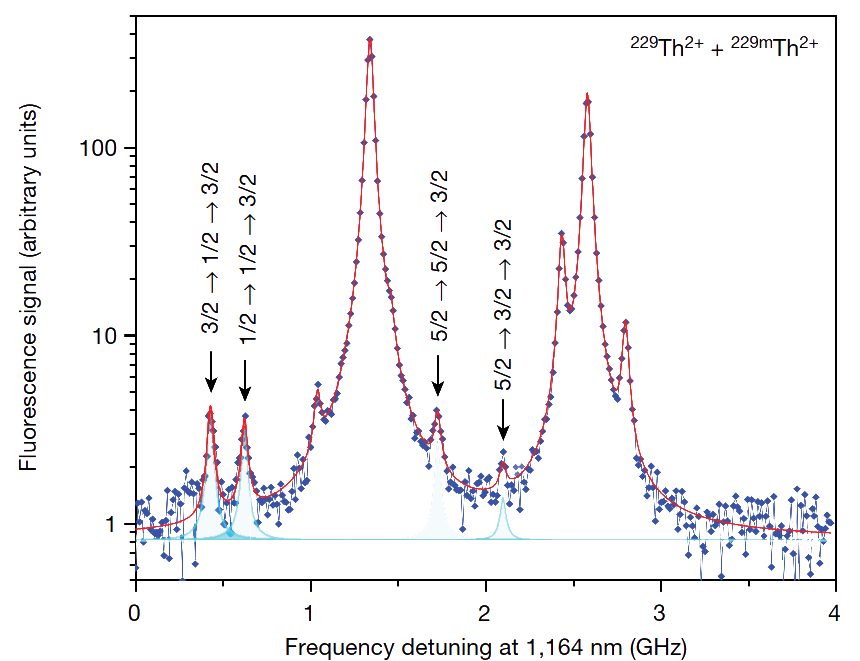
\includegraphics[width=.6\textwidth]{229spec.png}
	\end{textblock*}
	\begin{textblock*}{0.33\paperwidth}(0.05\paperwidth,0.3\paperheight)
		\centering
		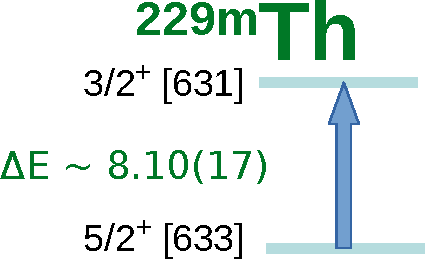
\includegraphics[width=\textwidth]{229Scheme.pdf}
	\end{textblock*}
	\begin{textblock*}{0.2\paperwidth}(0.82\paperwidth,0.5\paperheight)
		\textbf{Talks:}\\
		\colorbox{yellow}{S. Kraemer}\\
		\colorbox{yellow}{E. Peik}\\
		\colorbox{yellow}{R. Ferrer}\\
		\colorbox{yellow}{A. Claessens}\\
		\colorbox{yellow}{B. Seiferle}\\
	\end{textblock*}
	\begin{textblock*}{0.1\paperwidth}(0.05\paperwidth,0.7\paperheight)
		\footnote{ T. Sikorsky, PRL 125.14 (2020) 142503}
	\end{textblock*}
\end{frame}

\begin{frame}{Octupole Deformation and Charge Radii}
	\begin{textblock*}{0.9\paperwidth}(0.05\paperwidth,0.18\paperheight)
		\centering
		$\langle r^2 \rangle = \langle r^2 \rangle_{sph} \left( 1+\dfrac{5}{4 \pi}\left( \langle \beta^2_2\rangle+\langle \beta^2_3\rangle+...\right)\right)$
	\end{textblock*}
	\begin{textblock*}{0.4\paperwidth}(0.01\paperwidth,0.26\paperheight)
		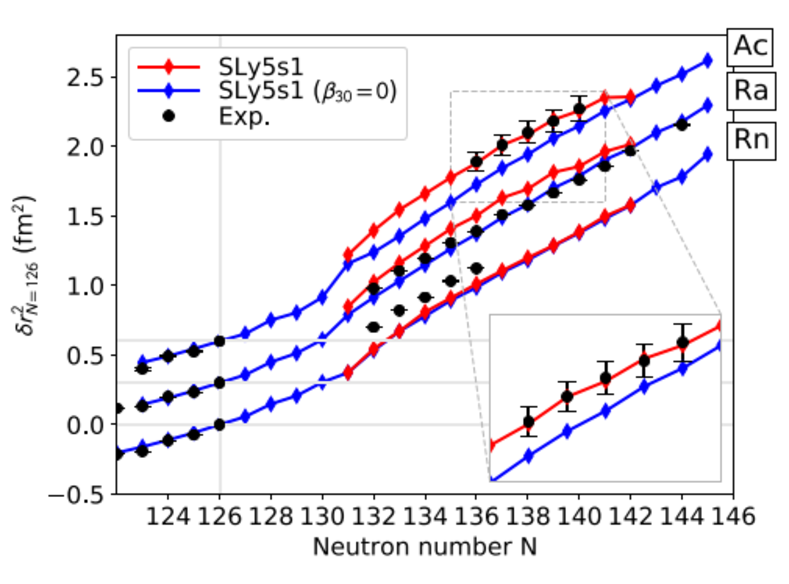
\includegraphics[width=\textwidth]{OctupoleBeta.pdf}
	\end{textblock*}
	\begin{textblock*}{0.1\paperwidth}(0.4\paperwidth,0.75\paperheight)
		\footnote{M. Bender, private communication}
	\end{textblock*}
	\begin{textblock*}{0.15\paperwidth}(0.4\paperwidth,0.26\paperheight)
		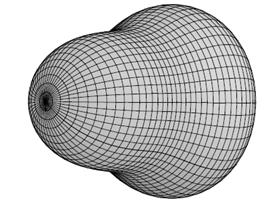
\includegraphics[width=\textwidth,angle=45]{OctupolePear.jpg}
	\end{textblock*}
	\begin{textblock*}{0.4\paperwidth}(0.6\paperwidth,0.28\paperheight)
		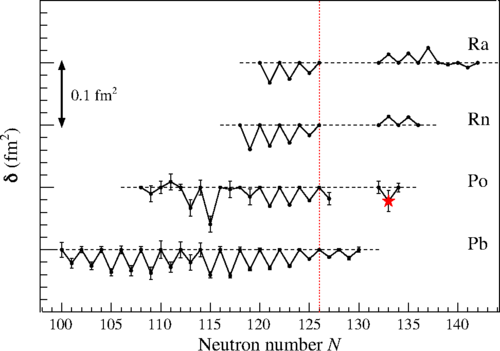
\includegraphics[width=0.65\textwidth]{OddEven.png}
	\end{textblock*}
	\begin{textblock*}{0.1\paperwidth}(0.9\paperwidth,0.62\paperheight)
		\footnote{D. Fink et al., PRX 5 (2015) 011018}
	\end{textblock*}
	\begin{textblock*}{0.6\paperwidth}(0.4\paperwidth,0.6\paperheight)
		\small	
		\begin{itemize}
				\item Comparison with EDF predictions. 
				\item Need to extend to heavier actinide experimental data
				\item Correlation between odd-even staggering reversal and octupole deformation?
				\item Collective behavior $\leftrightarrow$ enhancement of symmetry-violating nuclear properties
			\end{itemize}
	\end{textblock*}
\end{frame}


%----------------------------IGISOL---------------------------------
\begin{SectionTitle}
	\begin{frame}
		\centering
		\begin{textblock*}{0.5\paperwidth}(0.25\paperwidth,0.15\paperheight)
			\centering
			\textbf{\LARGE ACTINIDE QUEST AT IGISOL}	
		\end{textblock*}
		\begin{textblock*}{0.5\paperwidth}(0.25\paperwidth,0.4\paperheight)
			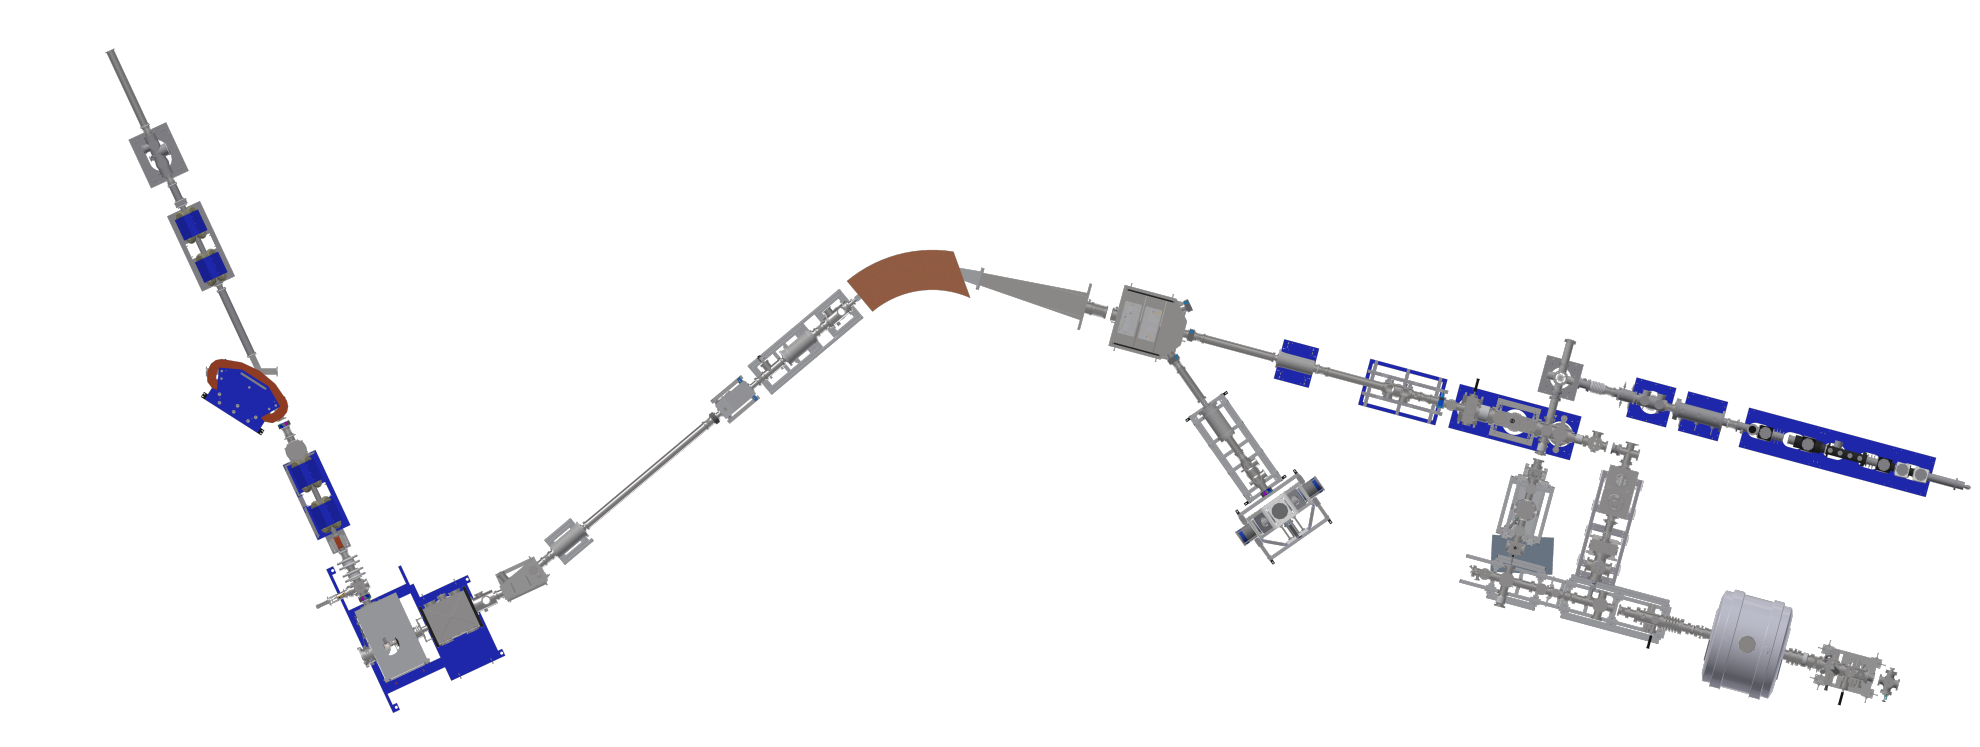
\includegraphics[width=.9\textwidth]{IGI-1A-IGISOL_3_no_logo.png}
		\end{textblock*}
	\end{frame}
\end{SectionTitle}

\begin{frame}{Offline Production}
	\begin{textblock*}{0.8\paperwidth}(0.01\paperwidth,0.1\paperheight)
		\only<1->{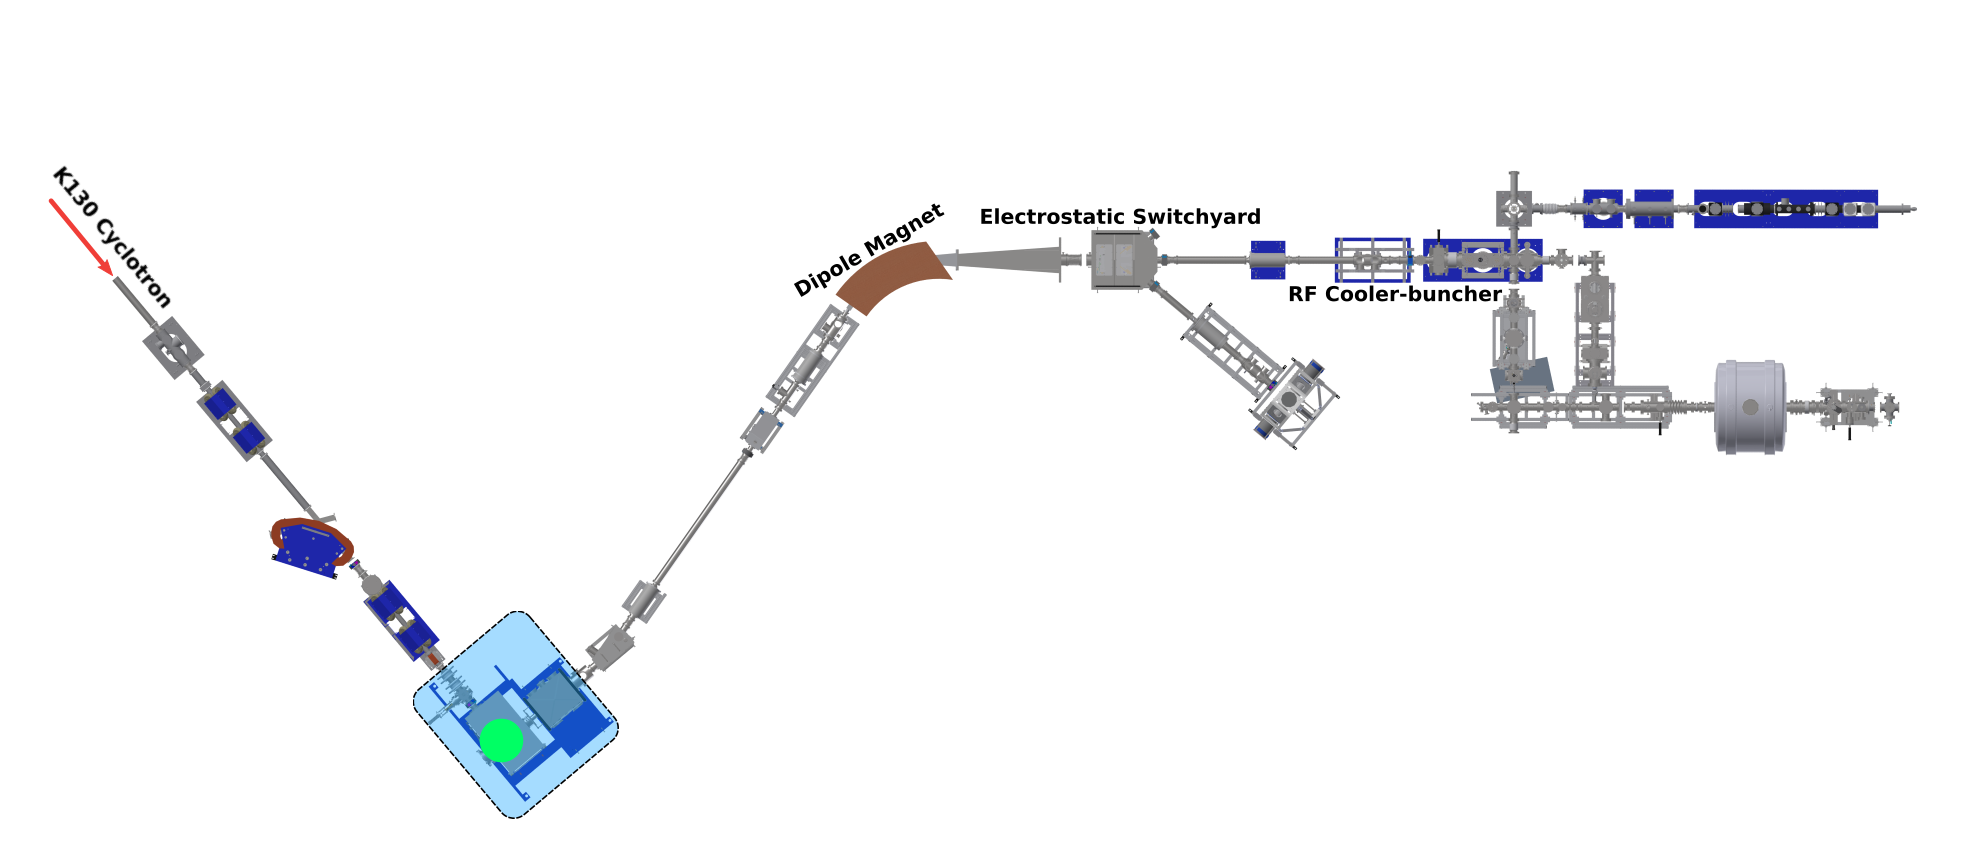
\includegraphics[width=\textwidth]{Igisol_scheme_TG.png}}%
	\end{textblock*}
	
	\begin{textblock*}{0.185\paperwidth}(0.13\paperwidth,0.17\paperheight)
		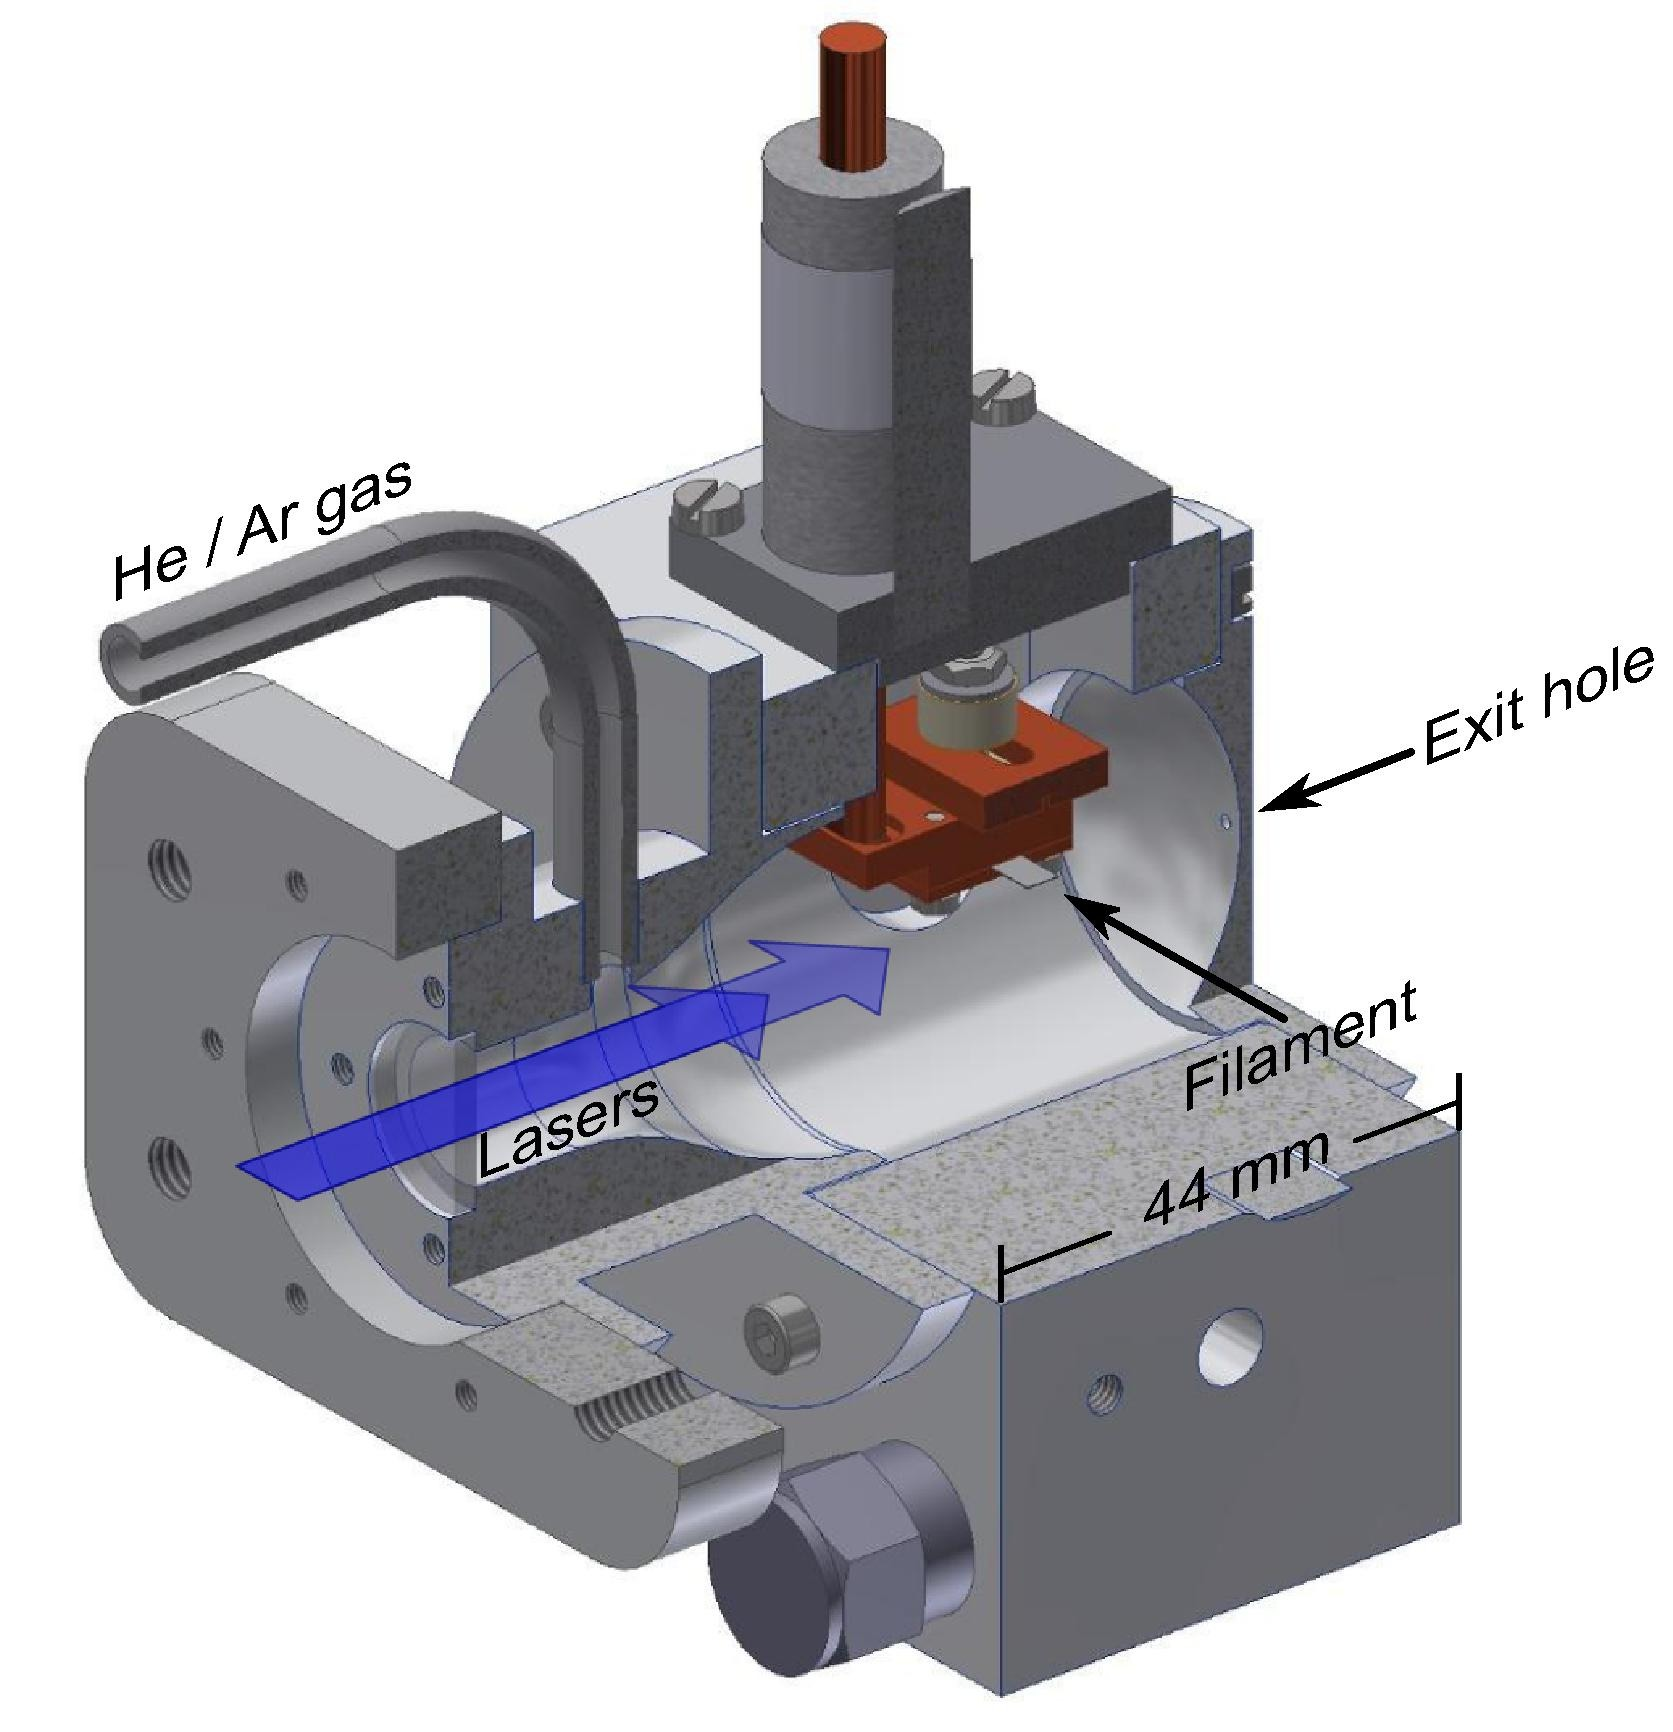
\includegraphics[width=0.8\textwidth]{PuGasCell.jpg}
	\end{textblock*}
	\begin{textblock*}{0.1\paperwidth}(0.82\paperwidth,0.2\paperheight)
		
\includegraphics[width=\textwidth]{jgu_logo_kasten.jpg}%
	\end{textblock*}
	\begin{textblock*}{0.7\paperwidth}(0.32\paperwidth,0.45\paperheight)
		\textbf{Resonance Ionization Spectroscopy and Gas Phase Chemistry}
	\end{textblock*}

	\begin{textblock*}{0.35\paperwidth}(0.62\paperwidth,0.52\paperheight)
		\textbf{Plutonium}
		\begin{itemize}
			\item Development of gas-cell for offline actinide studies
			\item $^{238-242,244}$Pu on Ta substrate, T=1100$^\circ$C
			\item Molecular formation in He and Ar buffer Gas
		\end{itemize}
	\end{textblock*}
	\begin{textblock*}{0.12\paperwidth}(0.02\paperwidth,0.55\paperheight)
		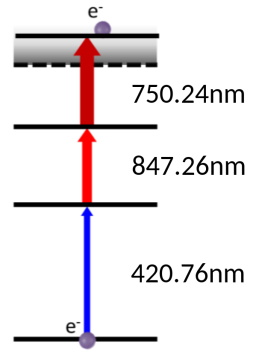
\includegraphics[width=\textwidth]{RIS.png}
	\end{textblock*}
	\begin{textblock*}{0.3\paperwidth}(0.3\paperwidth,0.52\paperheight)
		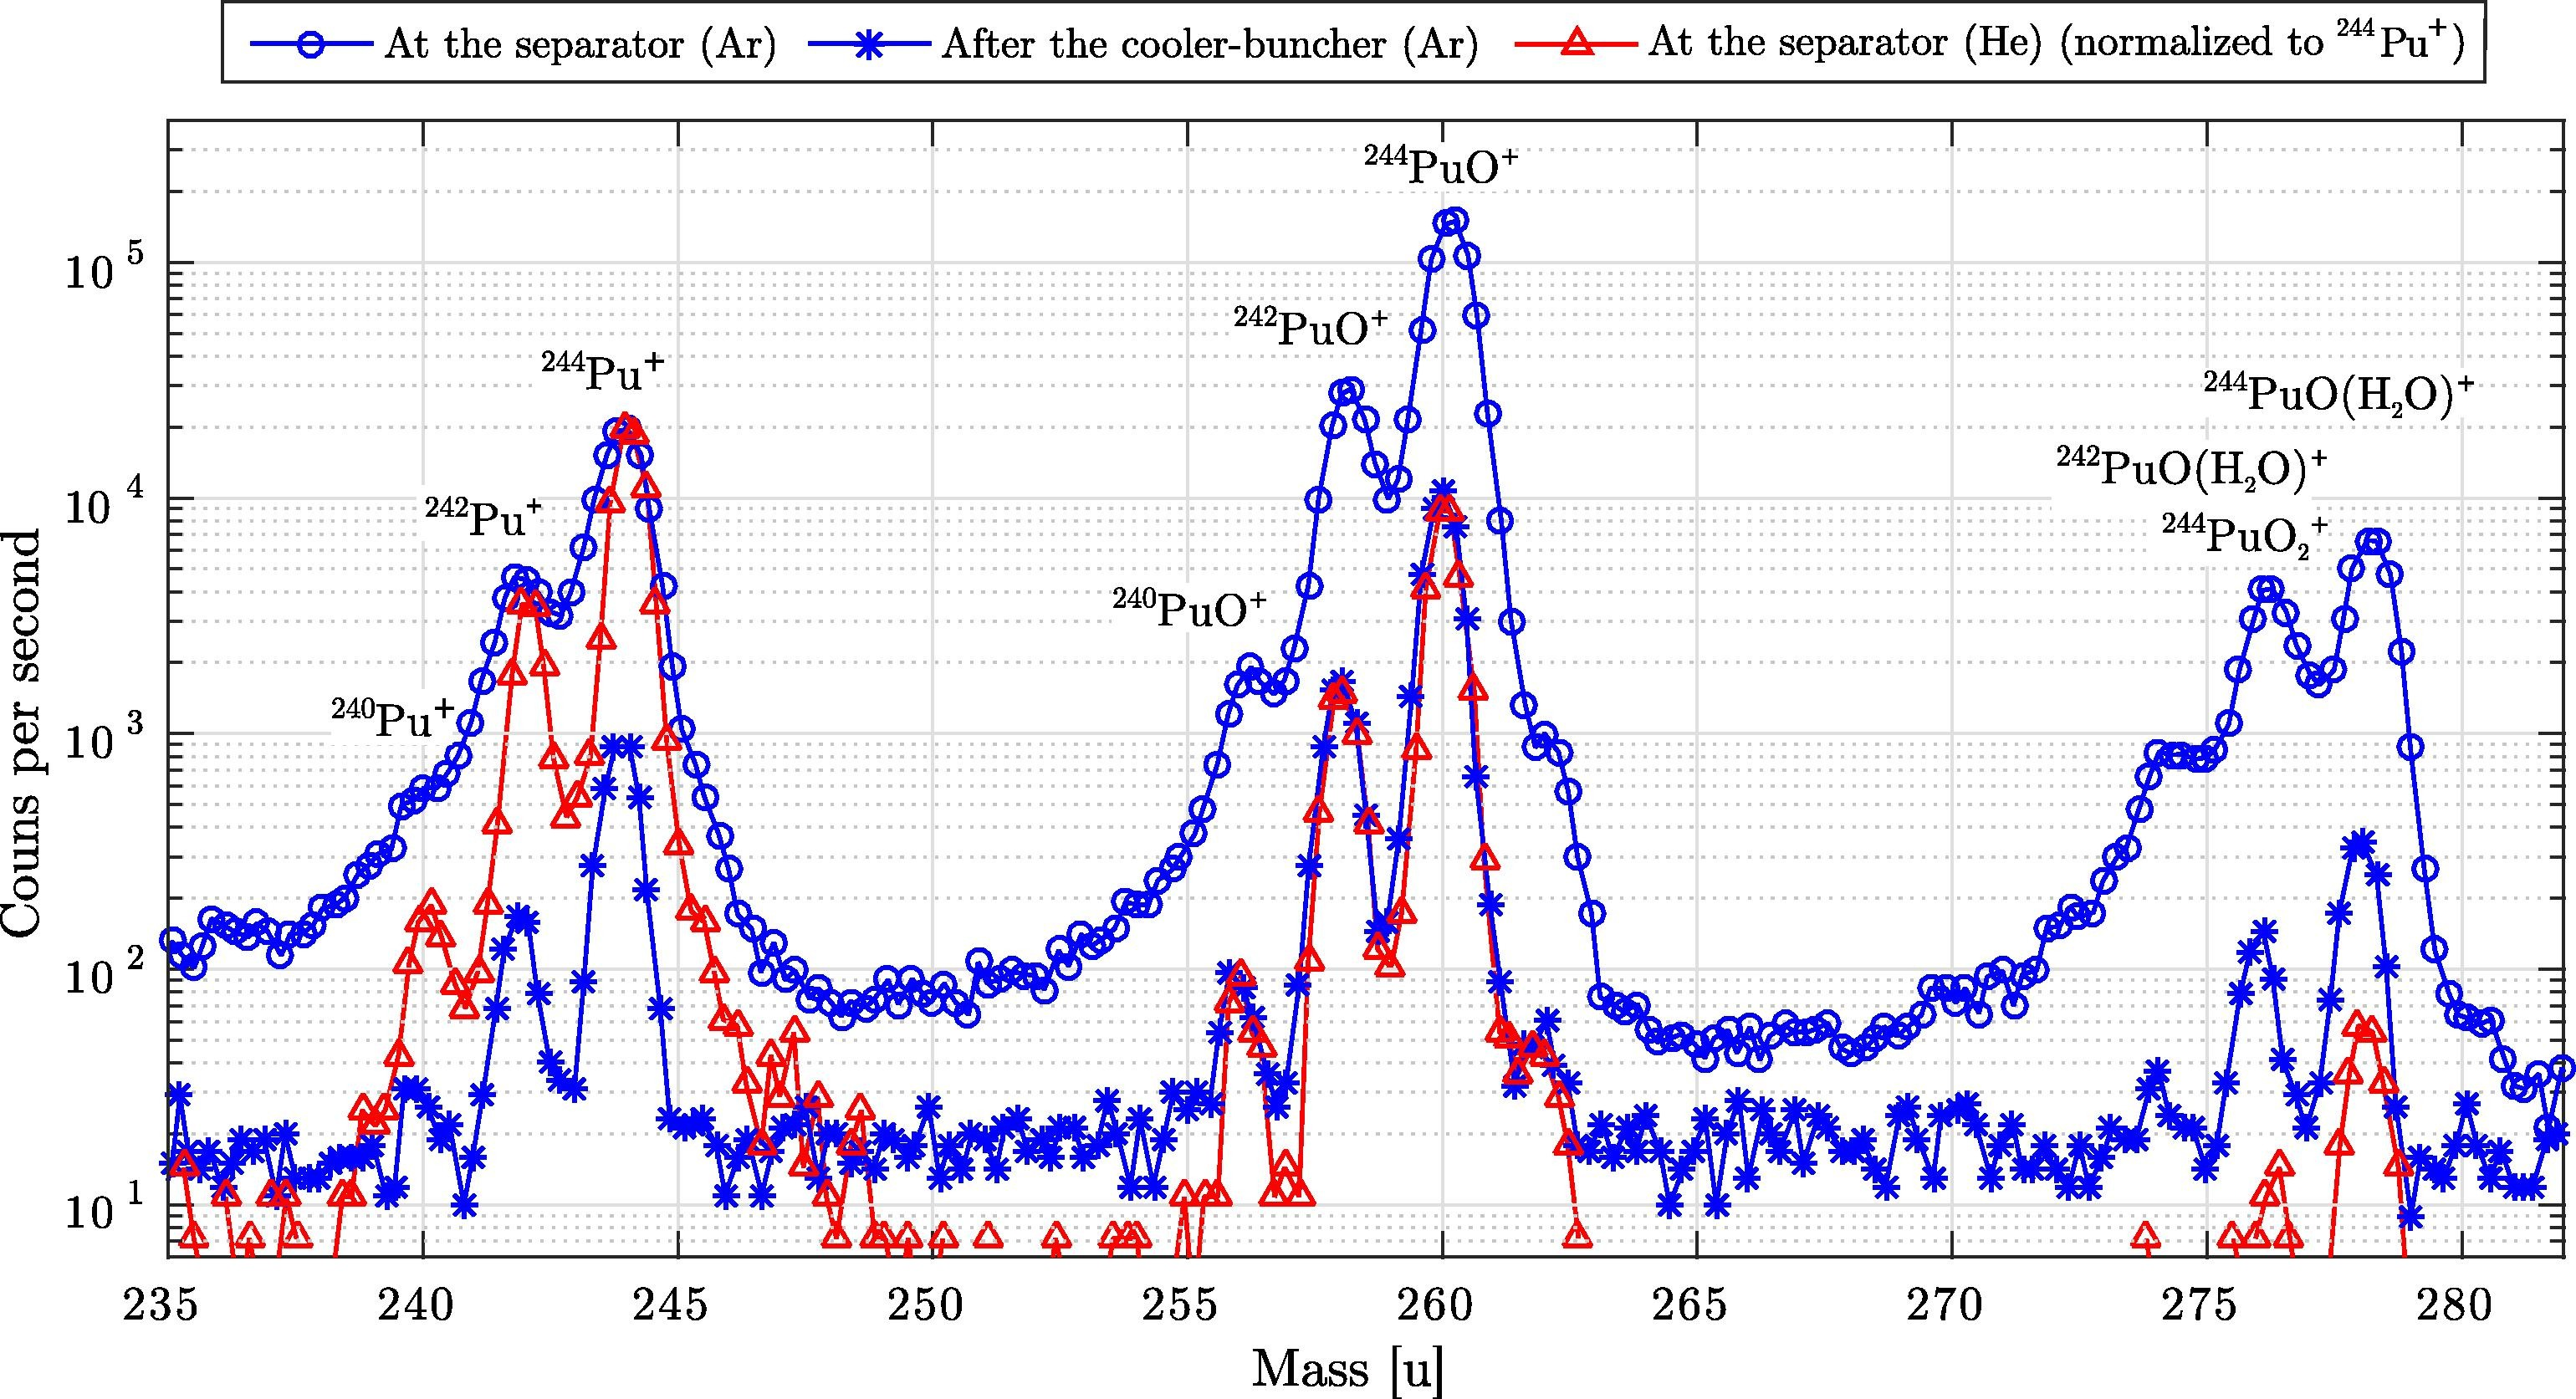
\includegraphics[width=\textwidth]{PuRIS.jpg}
	\end{textblock*}
	\begin{textblock*}{0.1\paperwidth}(0.61\paperwidth,0.8\paperheight)
		\footnote{I. Pohjalainen, NIM B 376 (2016) 233}
	\end{textblock*}
	
\end{frame}

\begin{frame}{Collinear Laser Spectroscopy}
	\begin{textblock*}{0.4\paperwidth}(0.01\paperwidth,0.2\paperheight)
		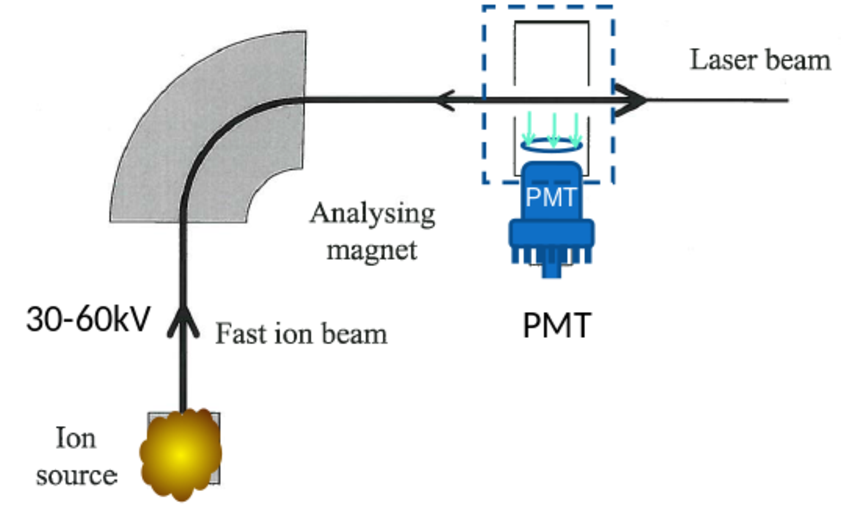
\includegraphics[width=\textwidth]{CLScheme.pdf}
	\end{textblock*}
	\begin{textblock*}{0.3\paperwidth}(0.05\paperwidth,0.7\paperheight)
		$^{244}$Pu $\sim$ $10^{16}$ at.\\
		$^{239}$Pu $\sim$ $2\times10^{14}$ at.\\
		$^{238}$Pu $\sim$ $2\times10^{12}$ at.\\
		\footnote{A. Voss, PRA 95 (2017) 032506}
	\end{textblock*}
	\only<1>{
		\begin{textblock*}{0.185\paperwidth}(0.3\paperwidth,0.5\paperheight)
			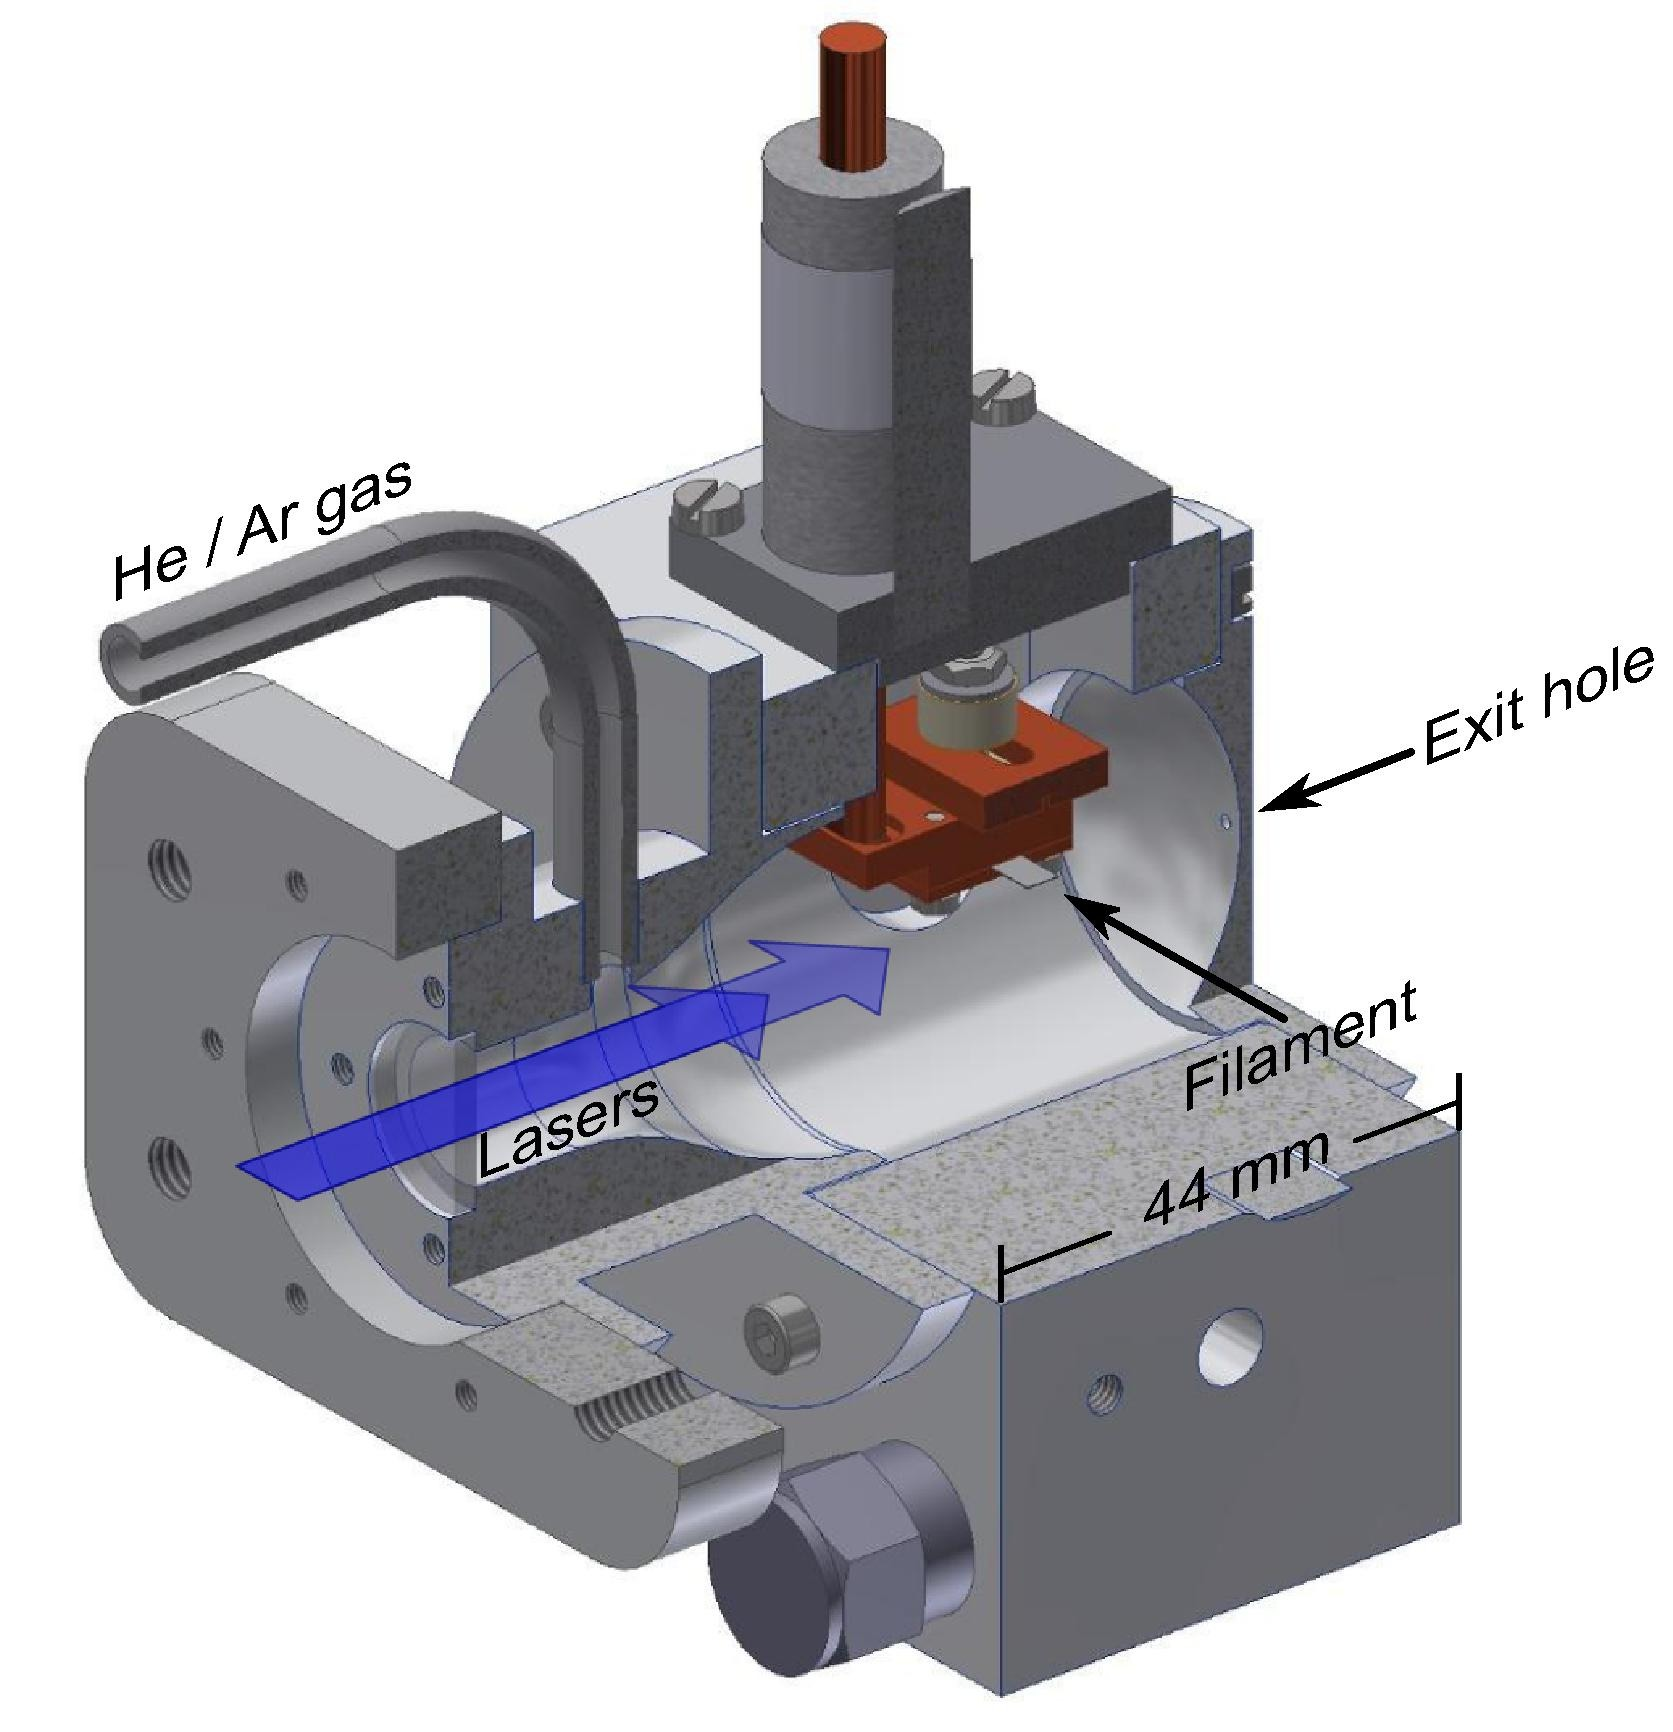
\includegraphics[width=0.8\textwidth]{PuGasCell.jpg}
		\end{textblock*}

		\begin{textblock*}{0.35\paperwidth}(0.52\paperwidth,0.48\paperheight)
			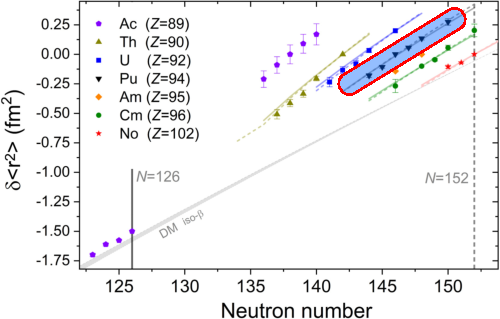
\includegraphics[width=\textwidth]{MSCR_PuHigh.jpg.pdf}
		\end{textblock*}
		
		\begin{textblock*}{0.5\paperwidth}(0.45\paperwidth,0.2\paperheight)
			\centering
			\textbf{Detection of fluorescence photons\\ emitted by a 30~kV beam}\\
			\small
			\begin{itemize}
				\item Pu, heaviest element studied with CLS
				\item Measurement of isotope shifts and extraction of $\langle r^{2}\rangle$
			\end{itemize}
		\end{textblock*}
	}
	\only<2>{
		\begin{textblock*}{0.23\paperwidth}(0.7\paperwidth,0.2\paperheight)
			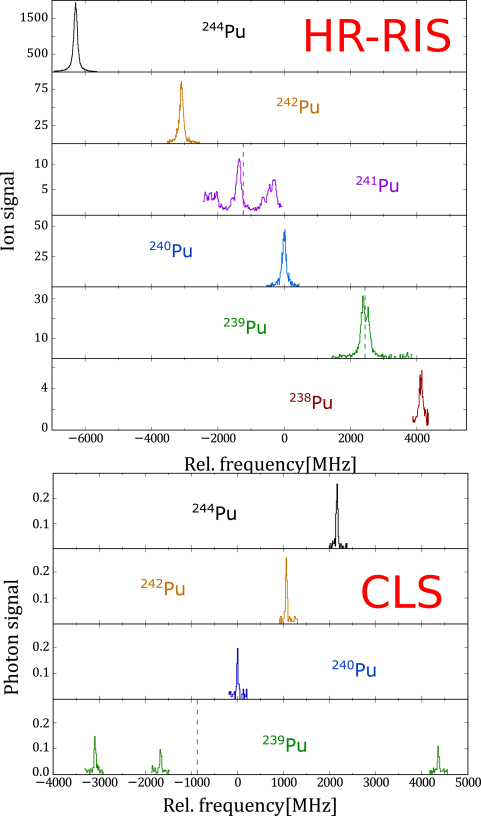
\includegraphics[width=\textwidth]{Pu_clsVsRis.png}\footnote{M. Block et al., PPNP, 116 (2021), 103834}
		\end{textblock*}
		\begin{textblock*}{0.35\paperwidth}(0.35\paperwidth,0.32\paperheight)
			\begin{itemize}
				\item Optimal agreement with\\HR-RIS technique
				\item systematic uncertainties on atomic factors dominates $\langle r^{2}\rangle$
				\item Atomic factor calibrated with king-plot method
			\end{itemize}
		\end{textblock*}
		\begin{textblock*}{0.3\paperwidth}(0.32\paperwidth,0.72\paperheight)
			$\delta \nu_i^{A,A^{\prime}} = M_i \dfrac{A^{\prime}-A}{A^{\prime}A} + F_i \delta\langle r^2\rangle^{A,A^{\prime}}$
		\end{textblock*}
		% \begin{textblock*}{0.6\paperwidth}(0.25\paperwidth,0.72\paperheight)
		% 	$\Delta E_{\text{hfs}}=\frac{1}{2}A_{\text{hfs}}C+B_{\text{hfs}}\frac{\frac{3}{2}C(C+1)-2I(I+1)J(J+1)}{2I(2I-1)2J(2J-1)}$
		% \end{textblock*}
		% \begin{textblock*}{0.6\paperwidth}(0.25\paperwidth,0.8\paperheight)
		% 	$C=F(F+1)-I(I+1)-J(J+1)$
		% \end{textblock*}
	}
	% \begin{textblock*}{0.2\paperwidth}(0.32\paperwidth,0.5\paperheight)
	% 	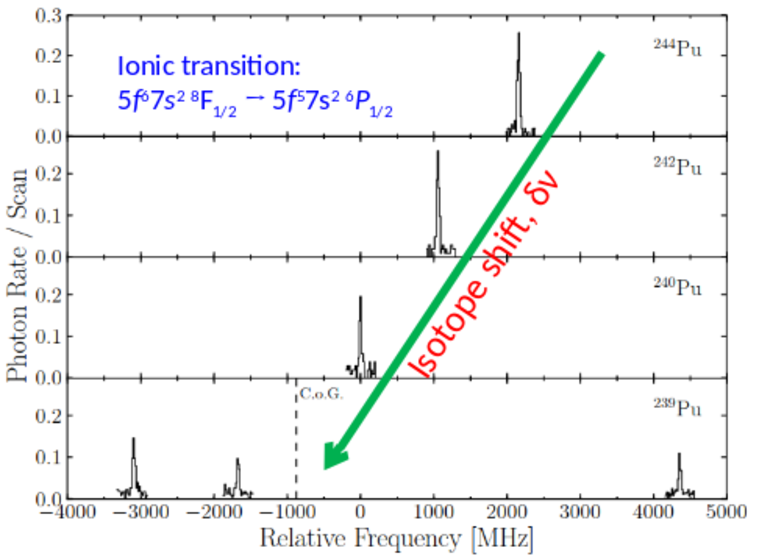
\includegraphics[width=\textwidth]{CLS_pu.pdf}
	% 	\footnote{A. Voss et al., PRA 95 (2017) 032506}
	% \end{textblock*}
	% \begin{textblock*}{0.3\paperwidth}(0.53\paperwidth,0.65\paperheight)
	% 	\small
	% 	\textbf{Plutonium}\\
	% 	Extraction of Field shifts\\ factors from King plot\\
	% \end{textblock*}
	

	
\end{frame}

\begin{frame}{Offline Production}
	\begin{textblock*}{0.8\paperwidth}(0.01\paperwidth,0.1\paperheight)
		\only<1->{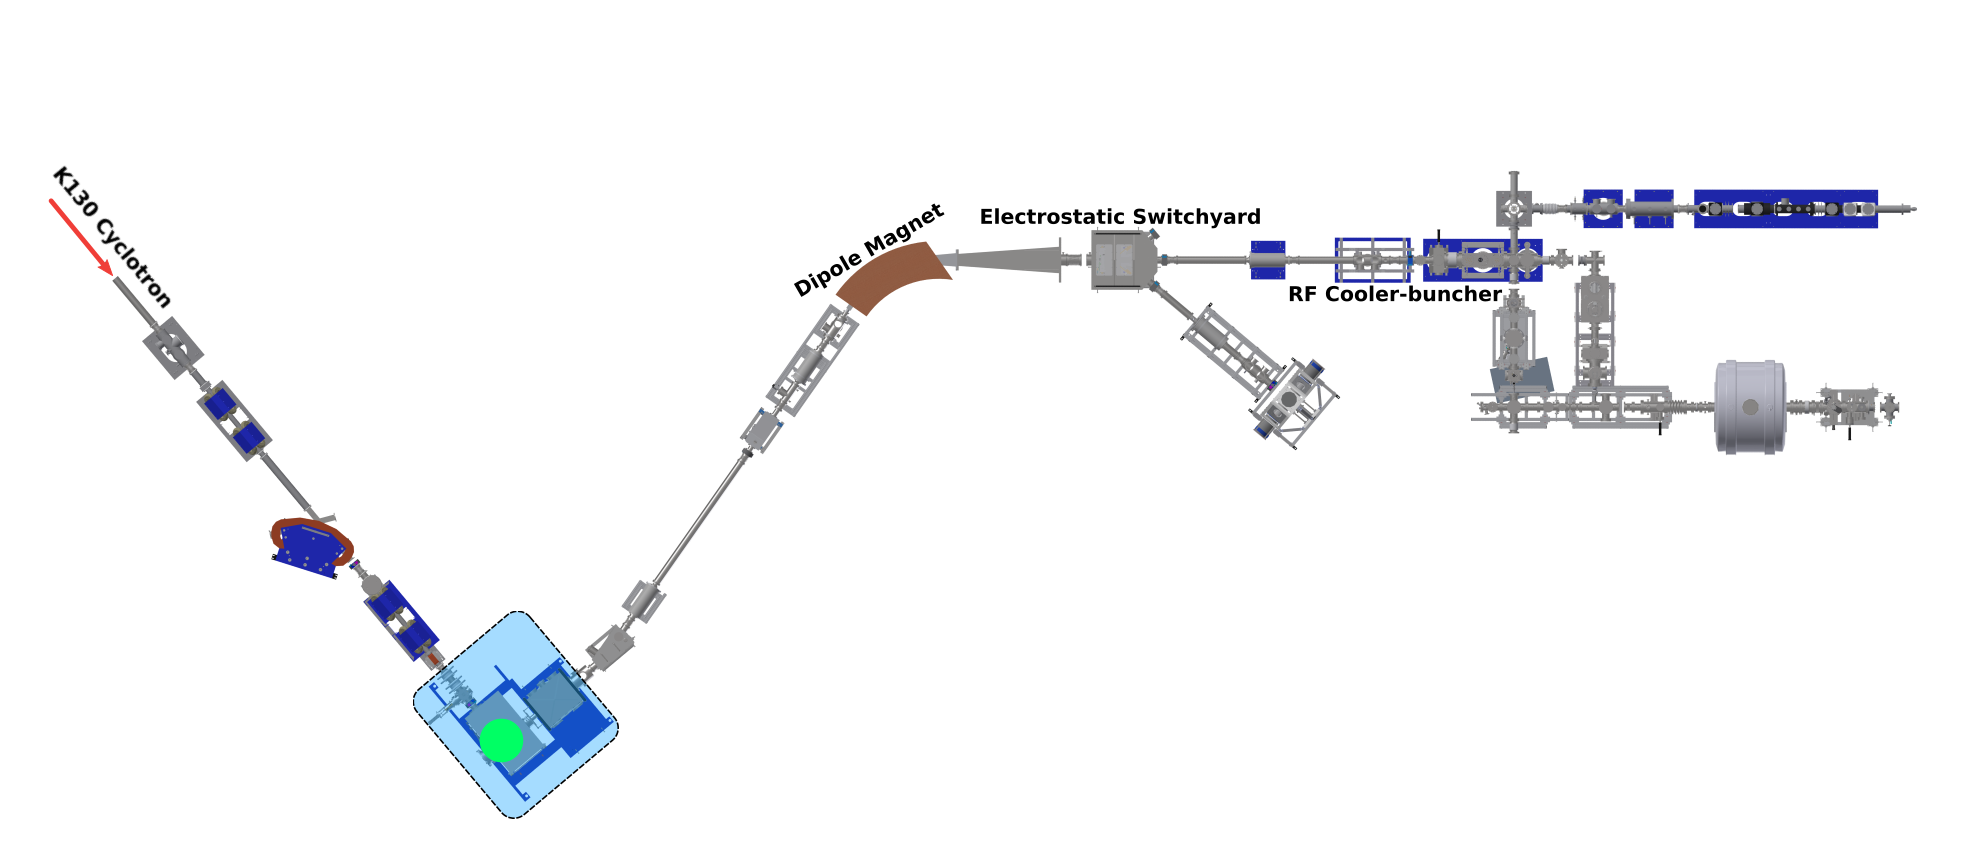
\includegraphics[width=\textwidth]{Igisol_scheme_TG.png}}%
	\end{textblock*}
	\begin{textblock*}{0.2\paperwidth}(0.7\paperwidth,0.04\paperheight)
		\only<1->{
\includegraphics[width=\textwidth]{nuclock.png}}%
	\end{textblock*}
	\begin{textblock*}{0.15\paperwidth}(0.8\paperwidth,0.25\paperheight)
		\only<1->{
\includegraphics[width=\textwidth]{TUwien.pdf}}%
	\end{textblock*}
	\begin{textblock*}{0.185\paperwidth}(0.12\paperwidth,0.17\paperheight)
		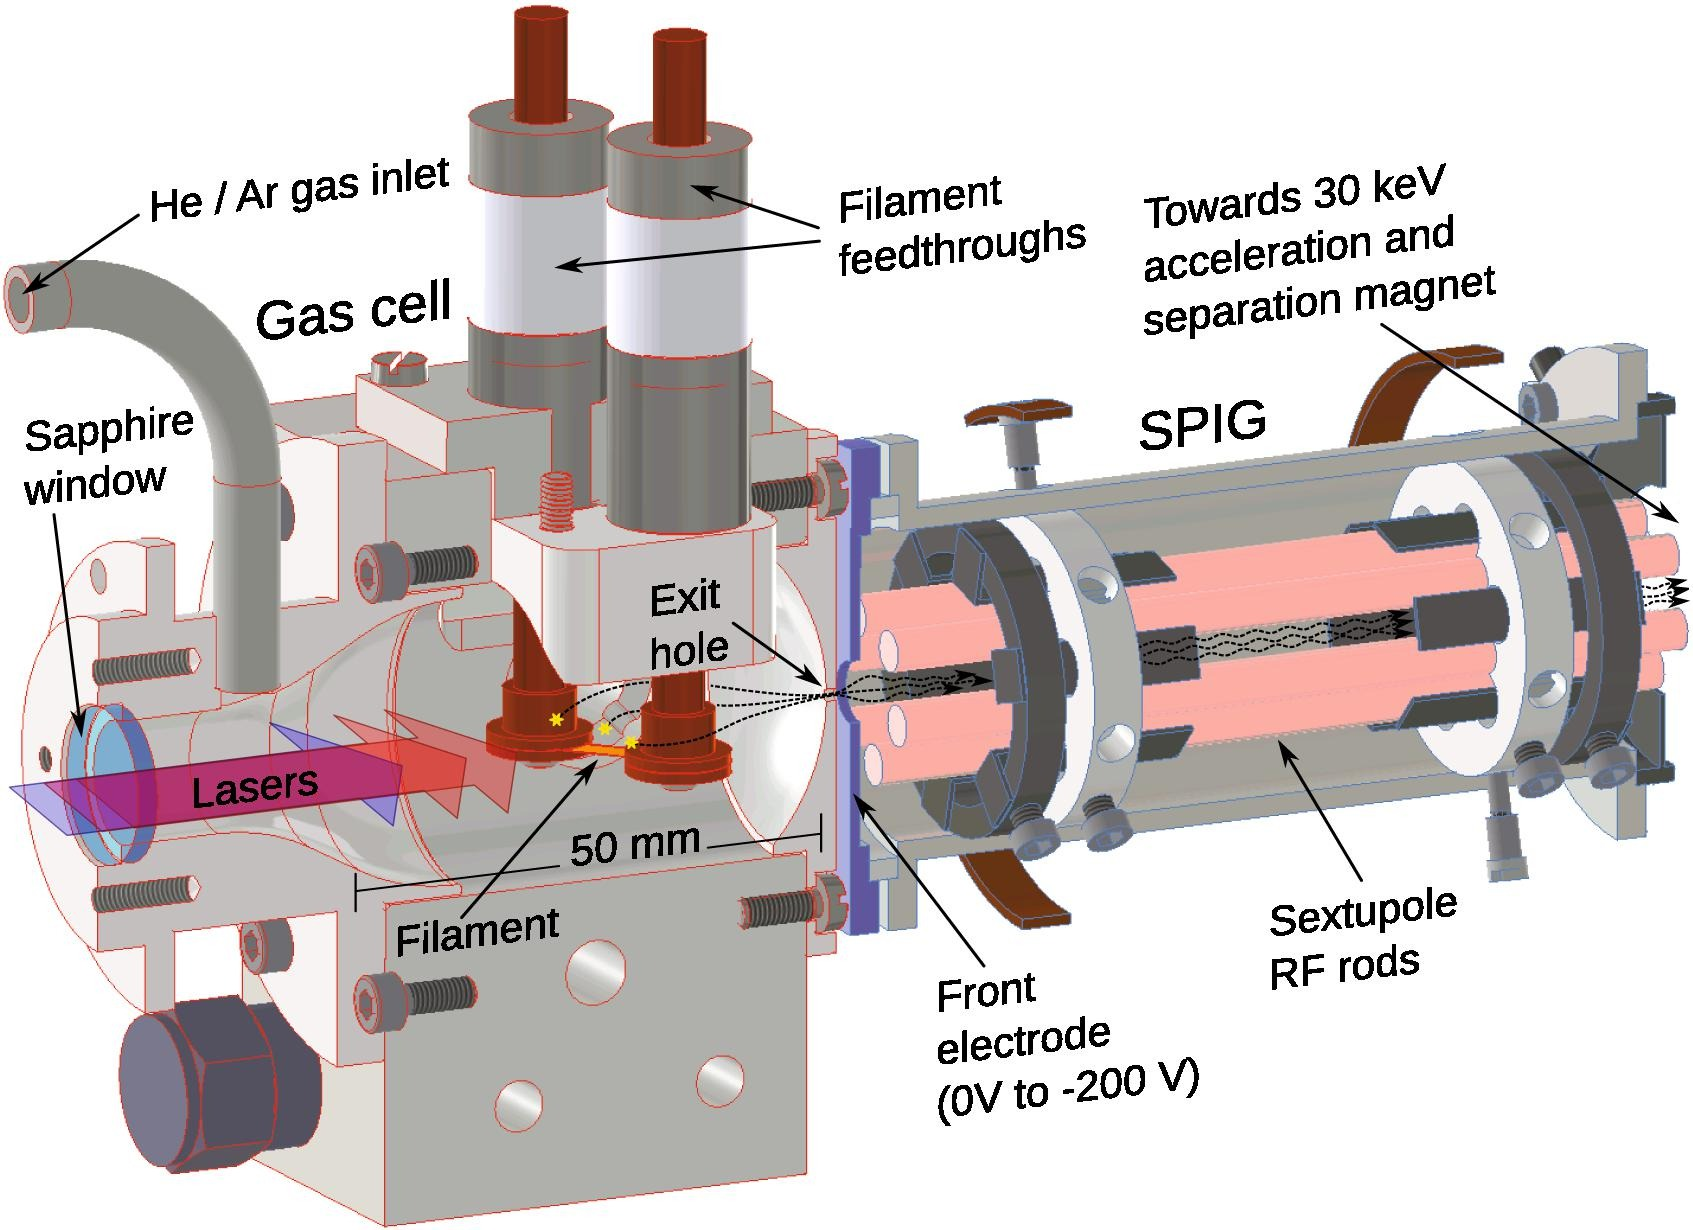
\includegraphics[width=\textwidth]{GasCell.jpg}
	\end{textblock*}
	\begin{textblock*}{0.1\paperwidth}(0.28\paperwidth,0.42\paperheight)
		\footnote{I. Pohjalainen, NIM B ,484 (2020) 59-70}
	\end{textblock*}

	\begin{textblock*}{0.7\paperwidth}(0.32\paperwidth,0.45\paperheight)
		\textbf{Development of a filament-based dispenser of Thorium}
	\end{textblock*}

	\begin{textblock*}{0.35\paperwidth}(0.62\paperwidth,0.55\paperheight)
		\begin{itemize}
			\item Thorium ion source for CLS experiments
			\item Challenging purity condition in gaseous environments
			\item Challenging filament production
		\end{itemize}
	\end{textblock*}
	\begin{textblock*}{0.15\paperwidth}(0.02\paperwidth,0.57\paperheight)
		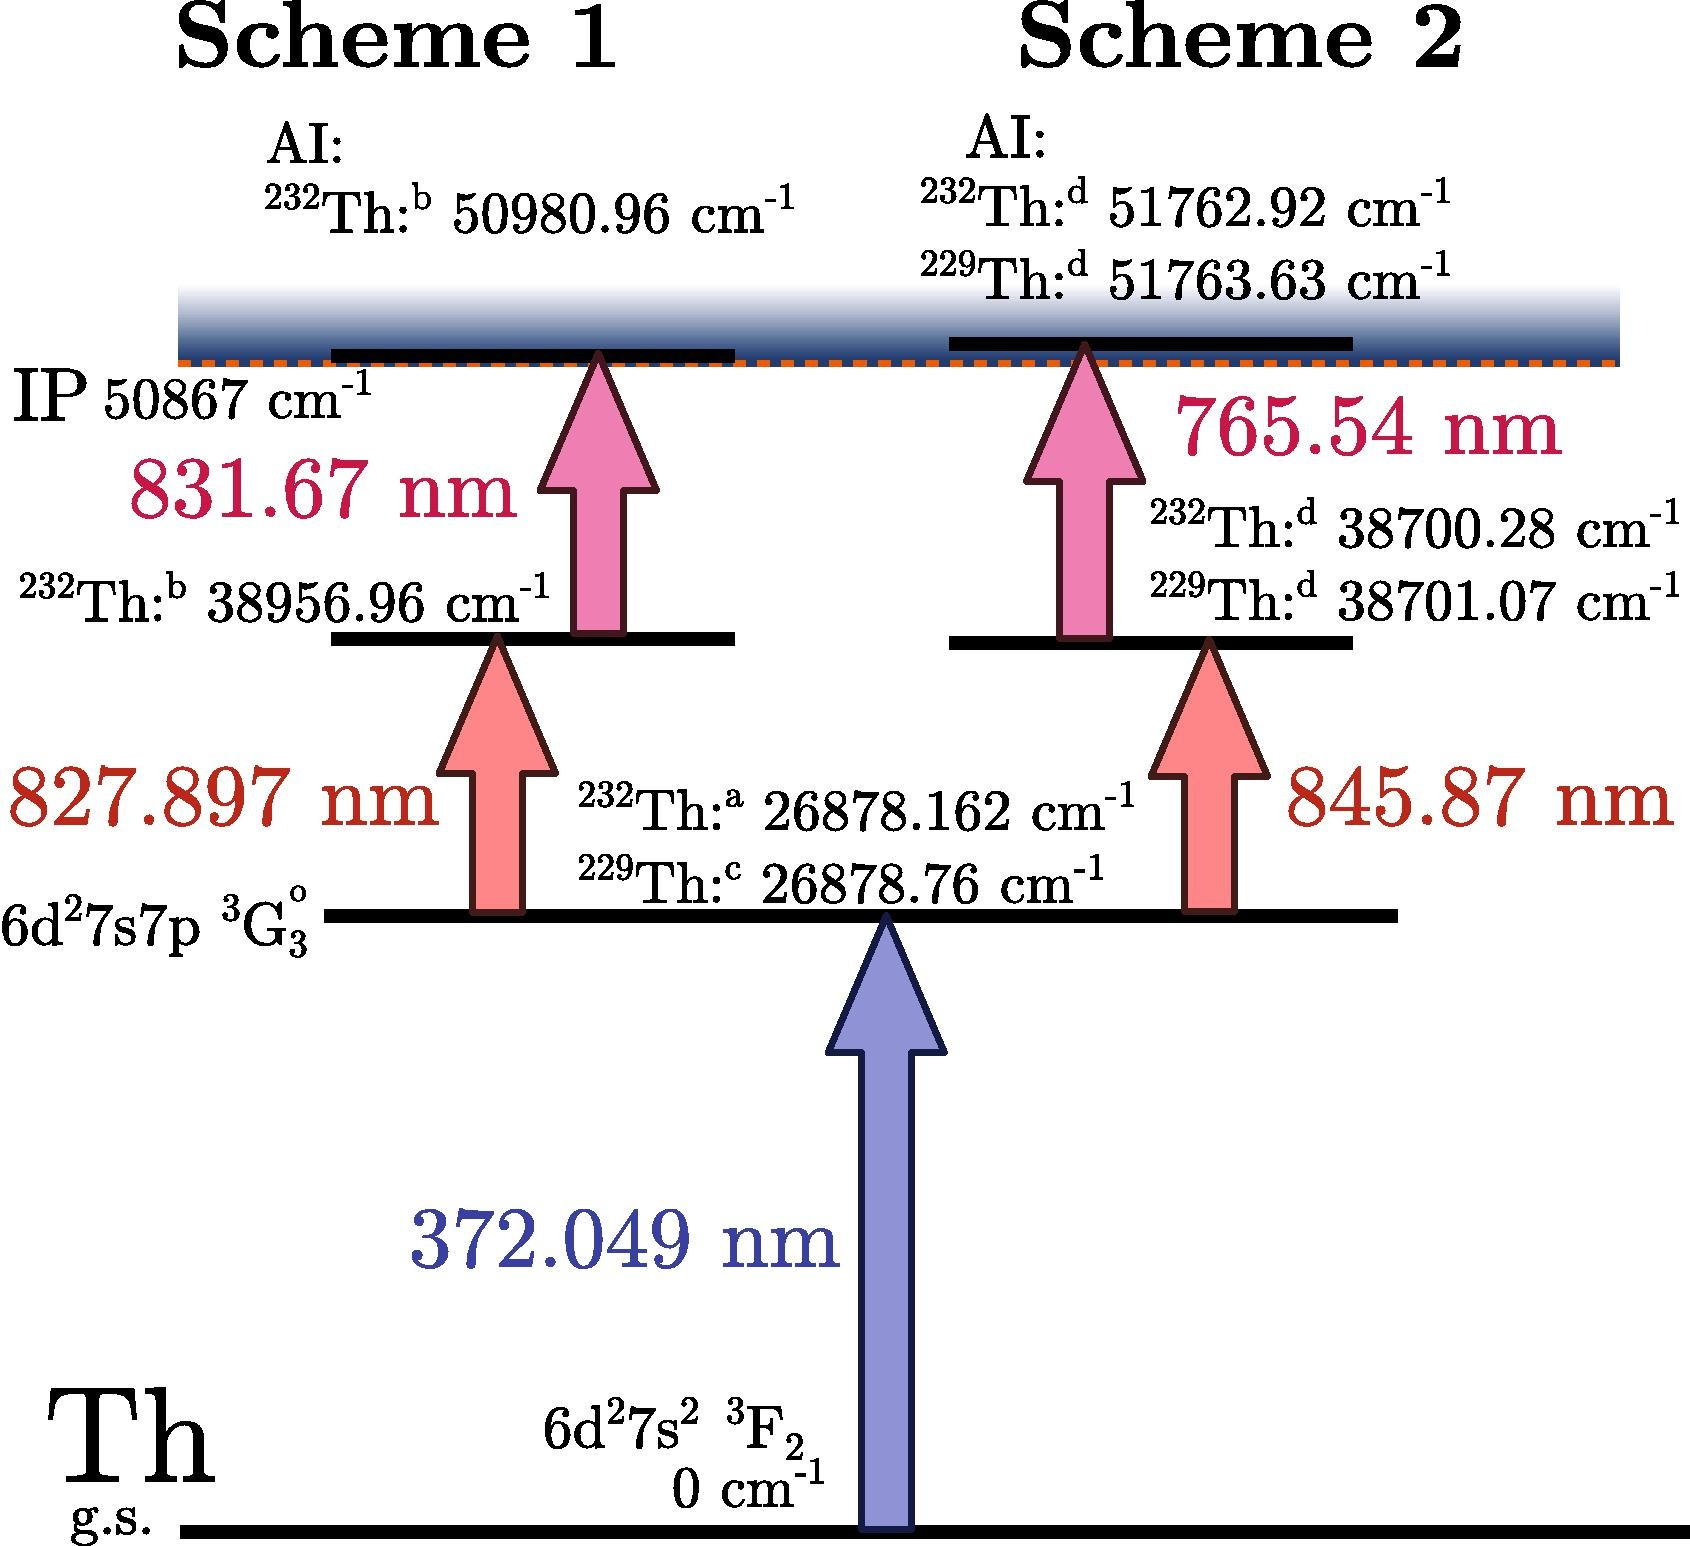
\includegraphics[width=\textwidth]{ThScheme.jpg}
	\end{textblock*}
	\begin{textblock*}{0.3\paperwidth}(0.3\paperwidth,0.52\paperheight)
		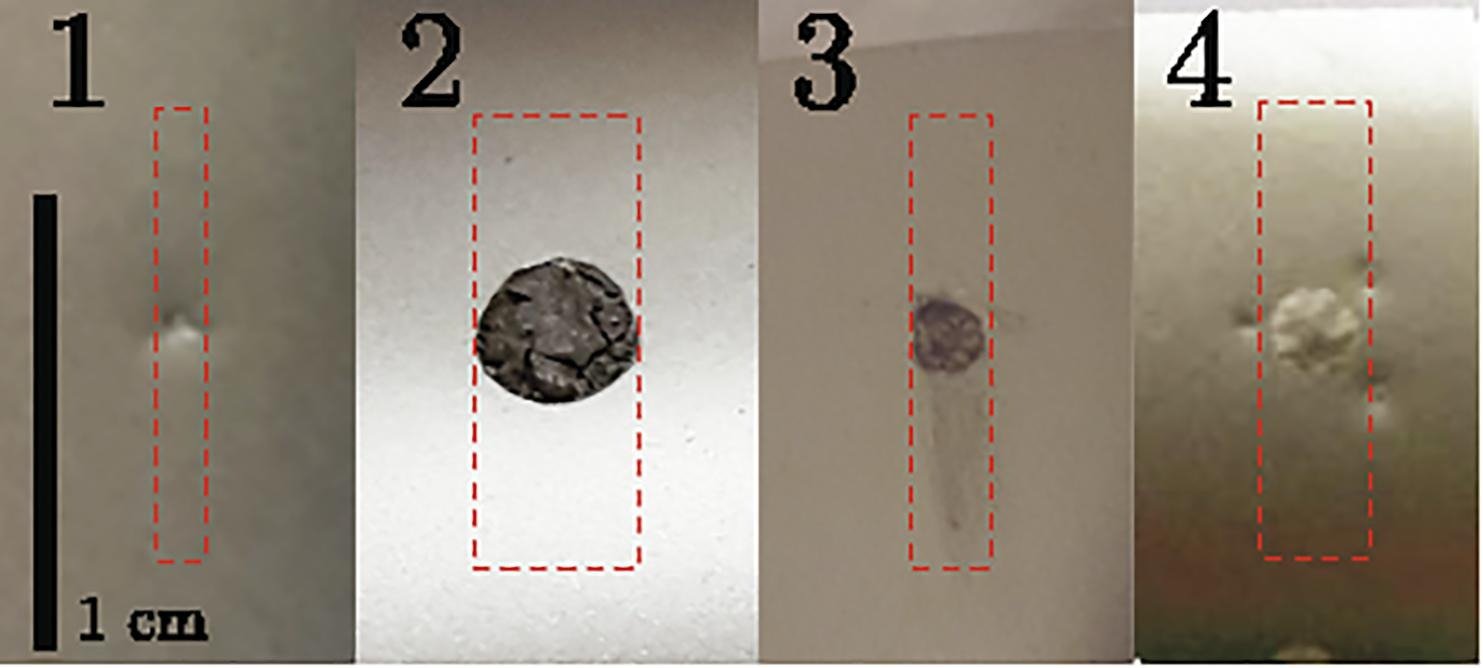
\includegraphics[width=\textwidth]{ThRIS.jpg}
	\end{textblock*}
	

\end{frame}


\begin{frame}{Offline Production}
	\begin{textblock*}{0.8\paperwidth}(0.01\paperwidth,0.1\paperheight)
		\only<1->{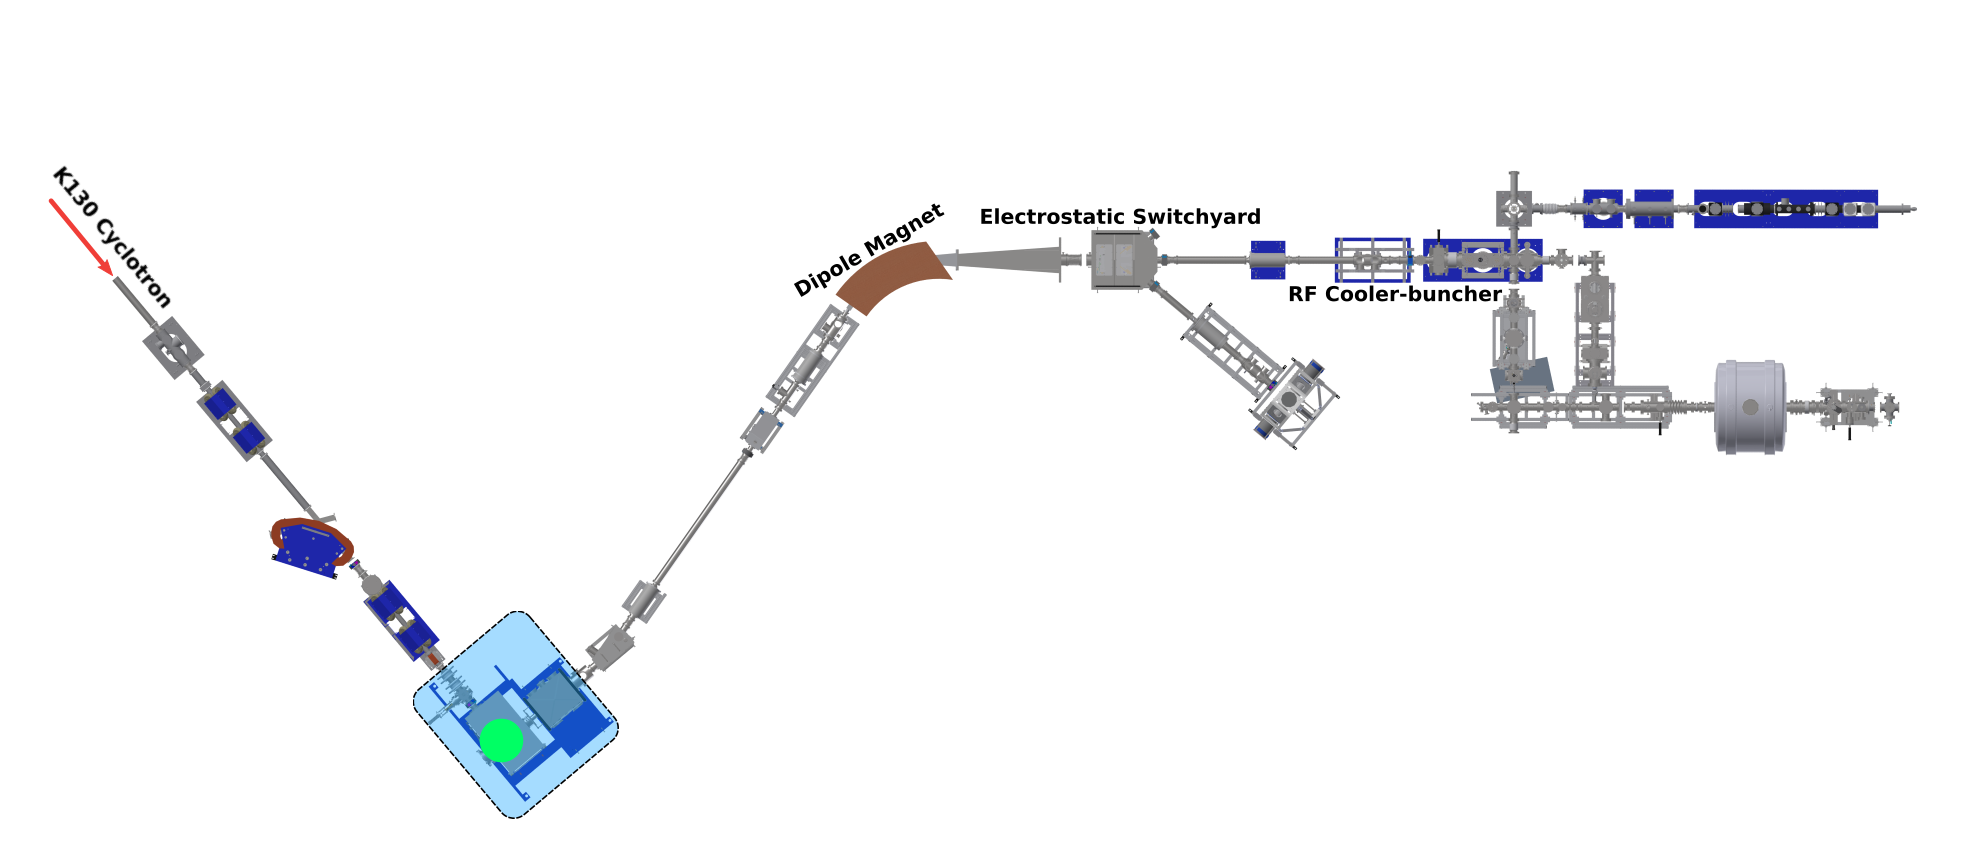
\includegraphics[width=\textwidth]{Igisol_scheme_TG.png}}%
	\end{textblock*}

	\begin{textblock*}{0.185\paperwidth}(0.12\paperwidth,0.17\paperheight)
		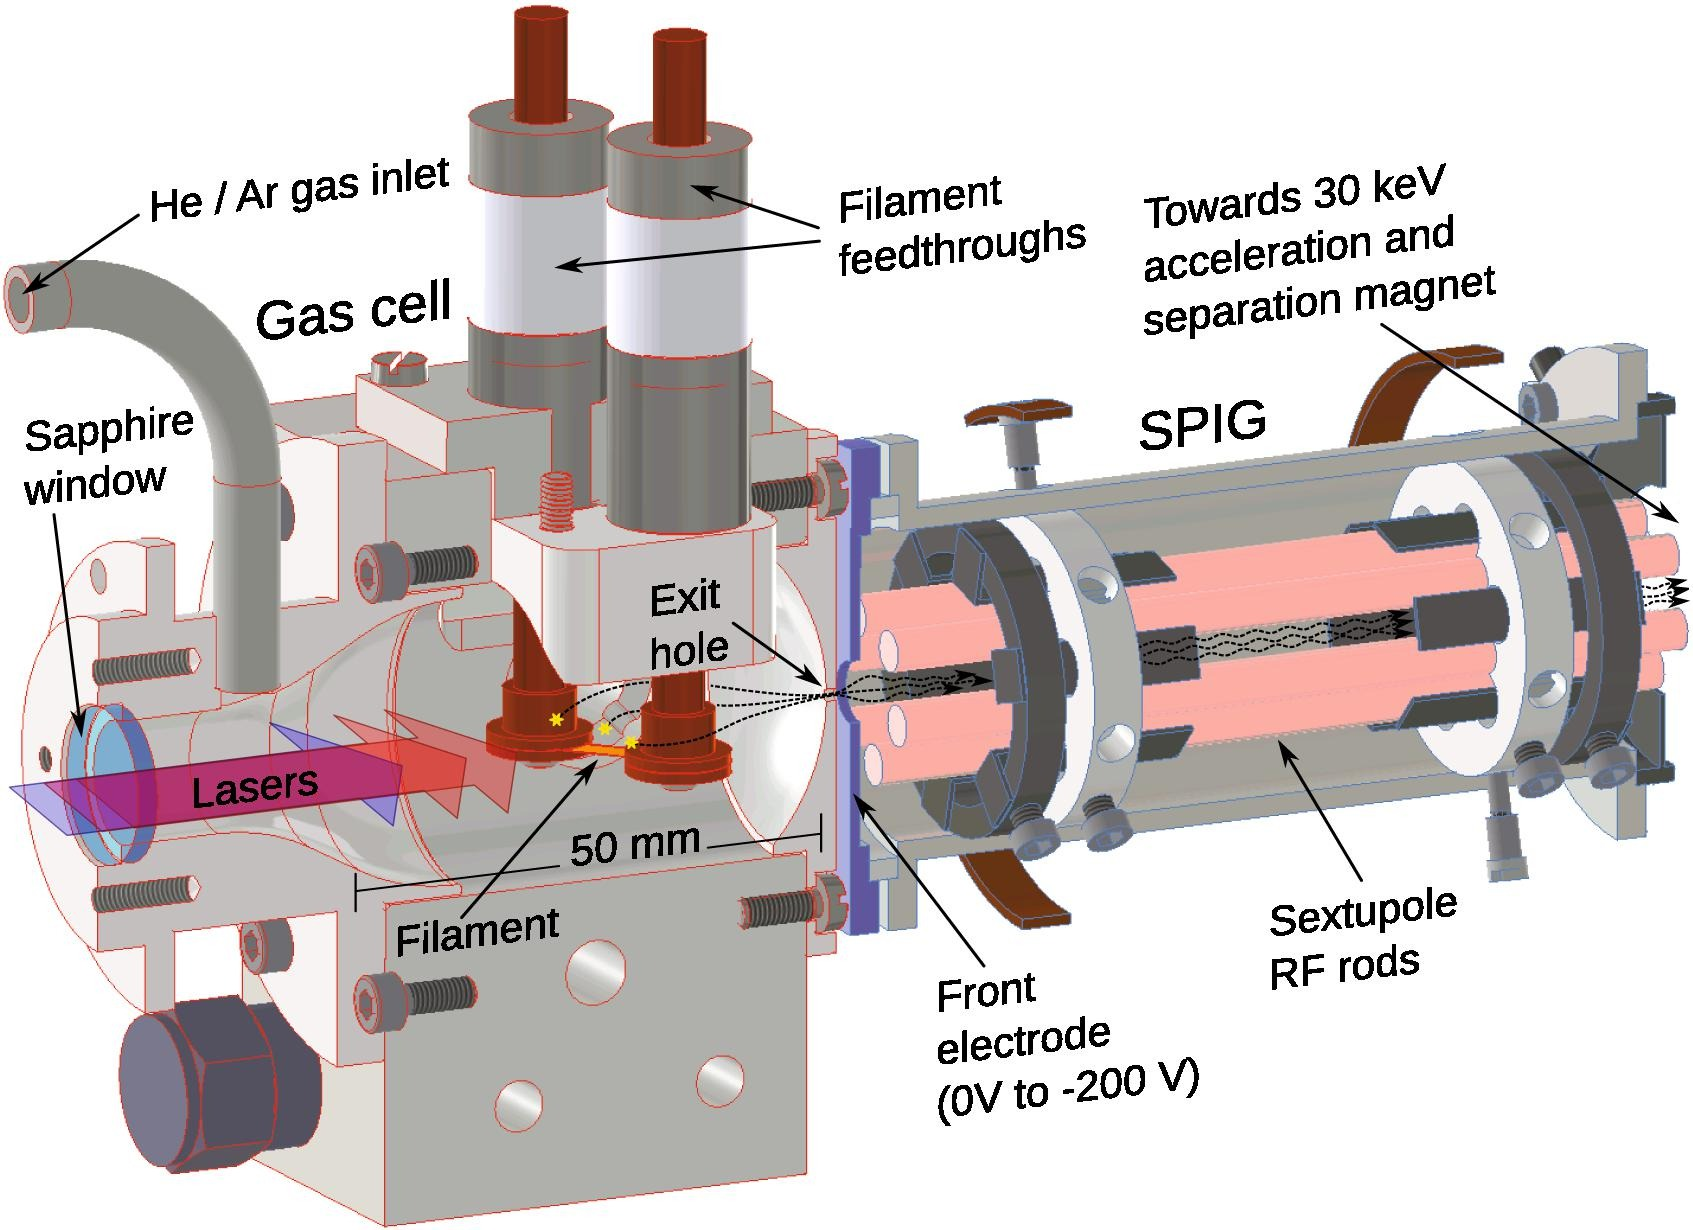
\includegraphics[width=\textwidth]{GasCell.jpg}
	\end{textblock*}
	\begin{textblock*}{0.1\paperwidth}(0.28\paperwidth,0.42\paperheight)
		\footnote{I. Pohjalainen, NIM B ,484 (2020) 59-70}
	\end{textblock*}
	\begin{textblock*}{0.1\paperwidth}(0.82\paperwidth,0.2\paperheight)
		\only<1->{
\includegraphics[width=\textwidth]{LMU.jpg}}%
	\end{textblock*}
	\begin{textblock*}{0.7\paperwidth}(0.4\paperwidth,0.45\paperheight)
		\textbf{Use of $^{233}$U as $^{229}$Th alpha recoil source}
	\end{textblock*}

	\begin{textblock*}{0.25\paperwidth}(0.72\paperwidth,0.5\paperheight)
		\small
		\begin{itemize}
			\item Study of alpha recoil efficiency
			\item Source characterization from $\alpha$/$\gamma$ detection
			\item Impurity studied with RBS technique 
		\end{itemize}
	\end{textblock*}
	\begin{textblock*}{0.15\paperwidth}(0.02\paperwidth,0.55\paperheight)
		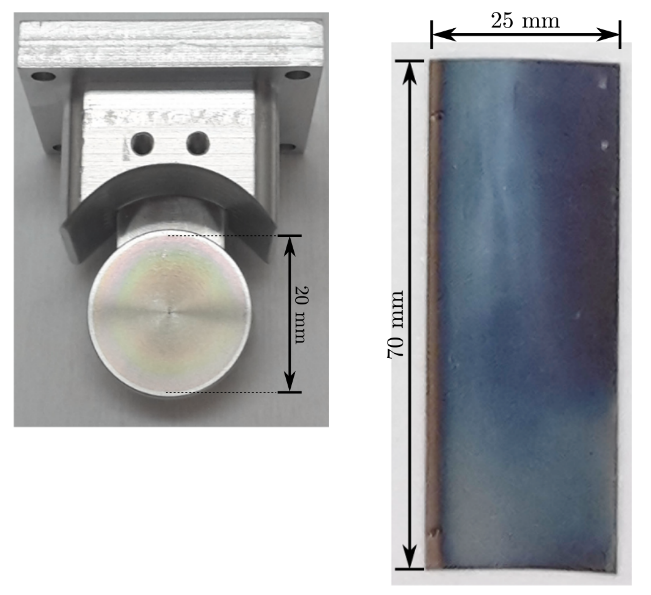
\includegraphics[width=\textwidth]{sources_comparison.png}
	\end{textblock*}
	\begin{textblock*}{0.22\paperwidth}(0.51\paperwidth,0.5\paperheight)
		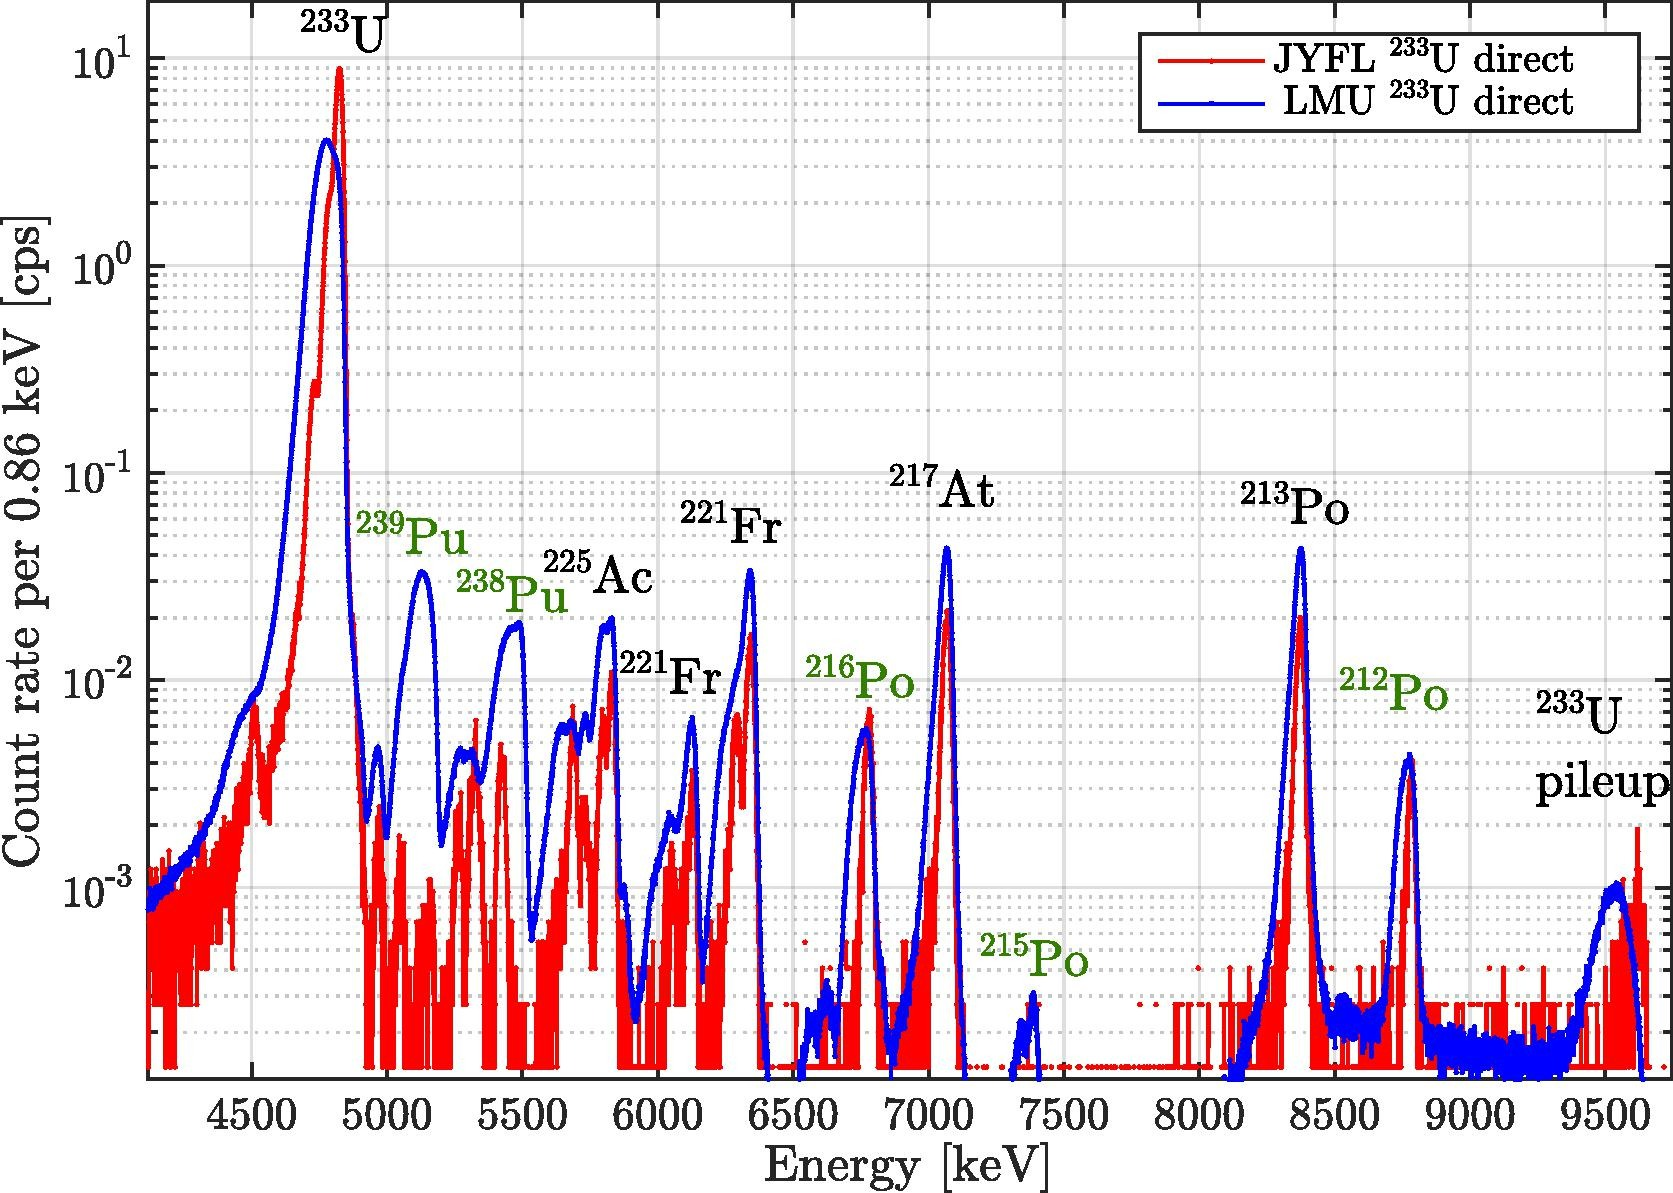
\includegraphics[width=\textwidth]{AlphaSpec.jpg}
	\end{textblock*}
	\begin{textblock*}{0.07\paperwidth}(0.05\paperwidth,0.75\paperheight)
		\footnote{I. Pohjalainen, NIM B ,463 (2020) 441-448}
	\end{textblock*}
	\begin{textblock*}{0.22\paperwidth}(0.28\paperwidth,0.51\paperheight)
		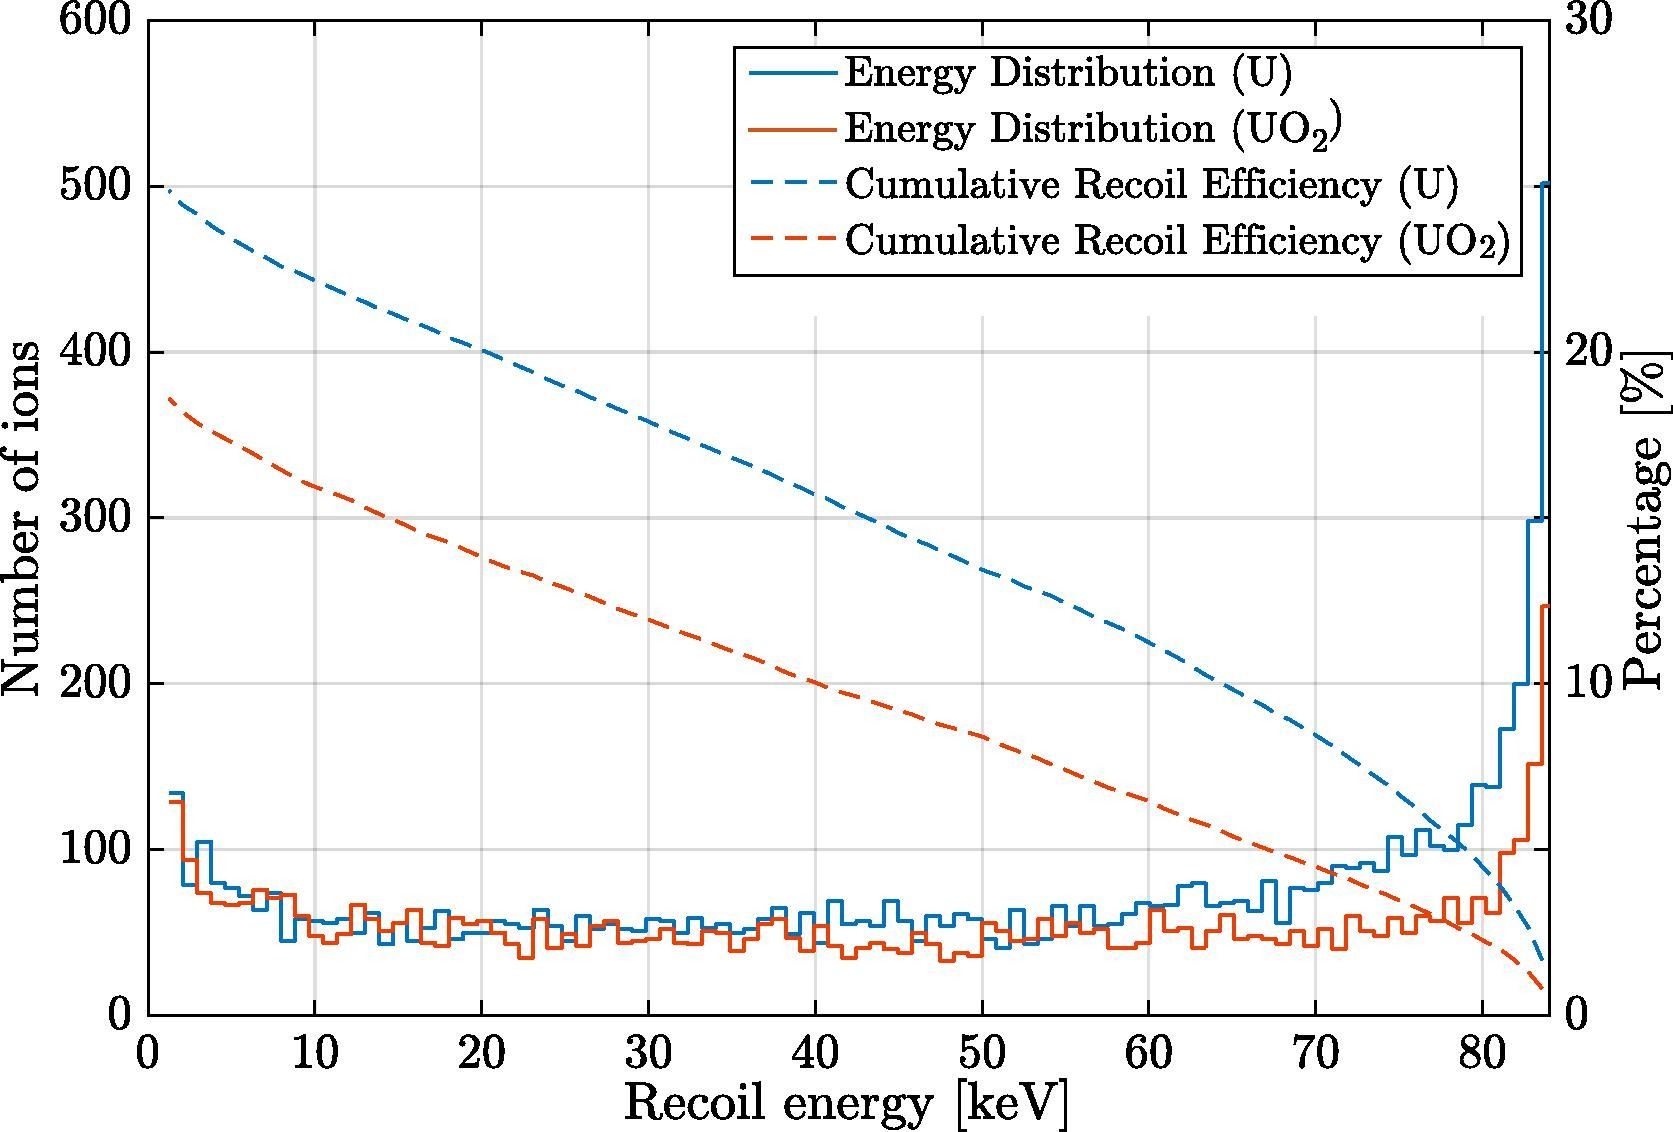
\includegraphics[width=\textwidth]{RecoilEfficiency.jpg}
	\end{textblock*}
\end{frame}

\begin{frame}{Online Production}
	\begin{textblock*}{0.8\paperwidth}(0.01\paperwidth,0.1\paperheight)
		% \only<1->{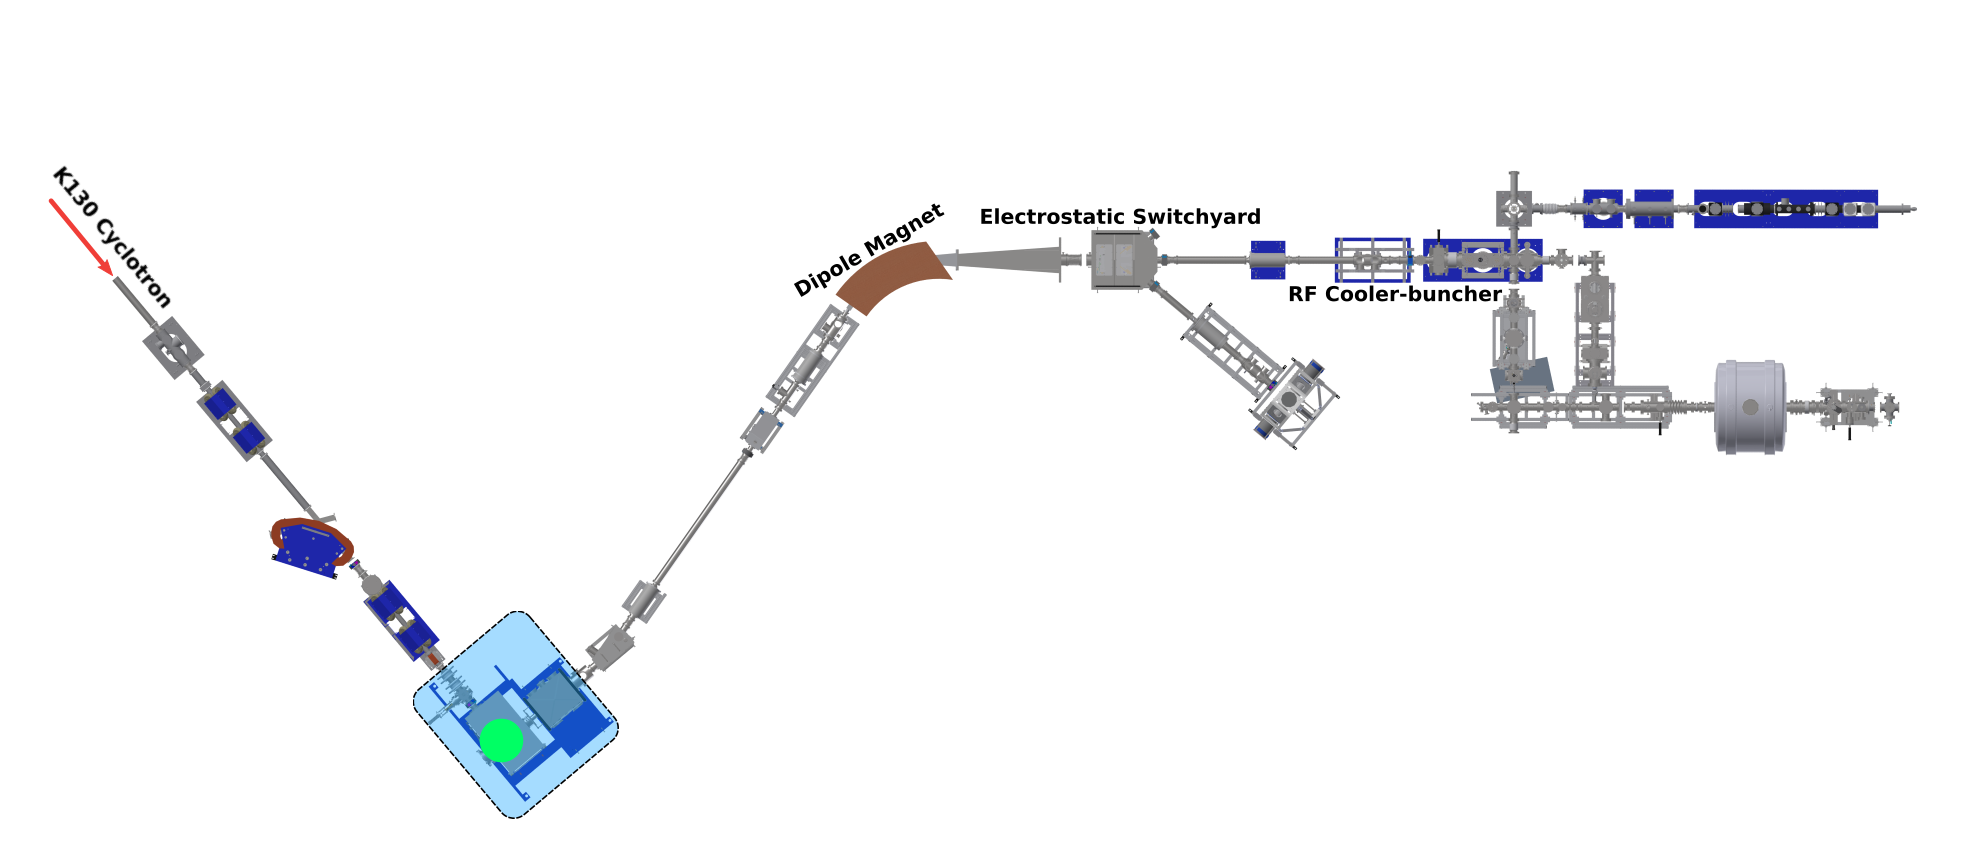
\includegraphics[width=\textwidth]{Igisol_scheme_TG.png}}%
		\only<1->{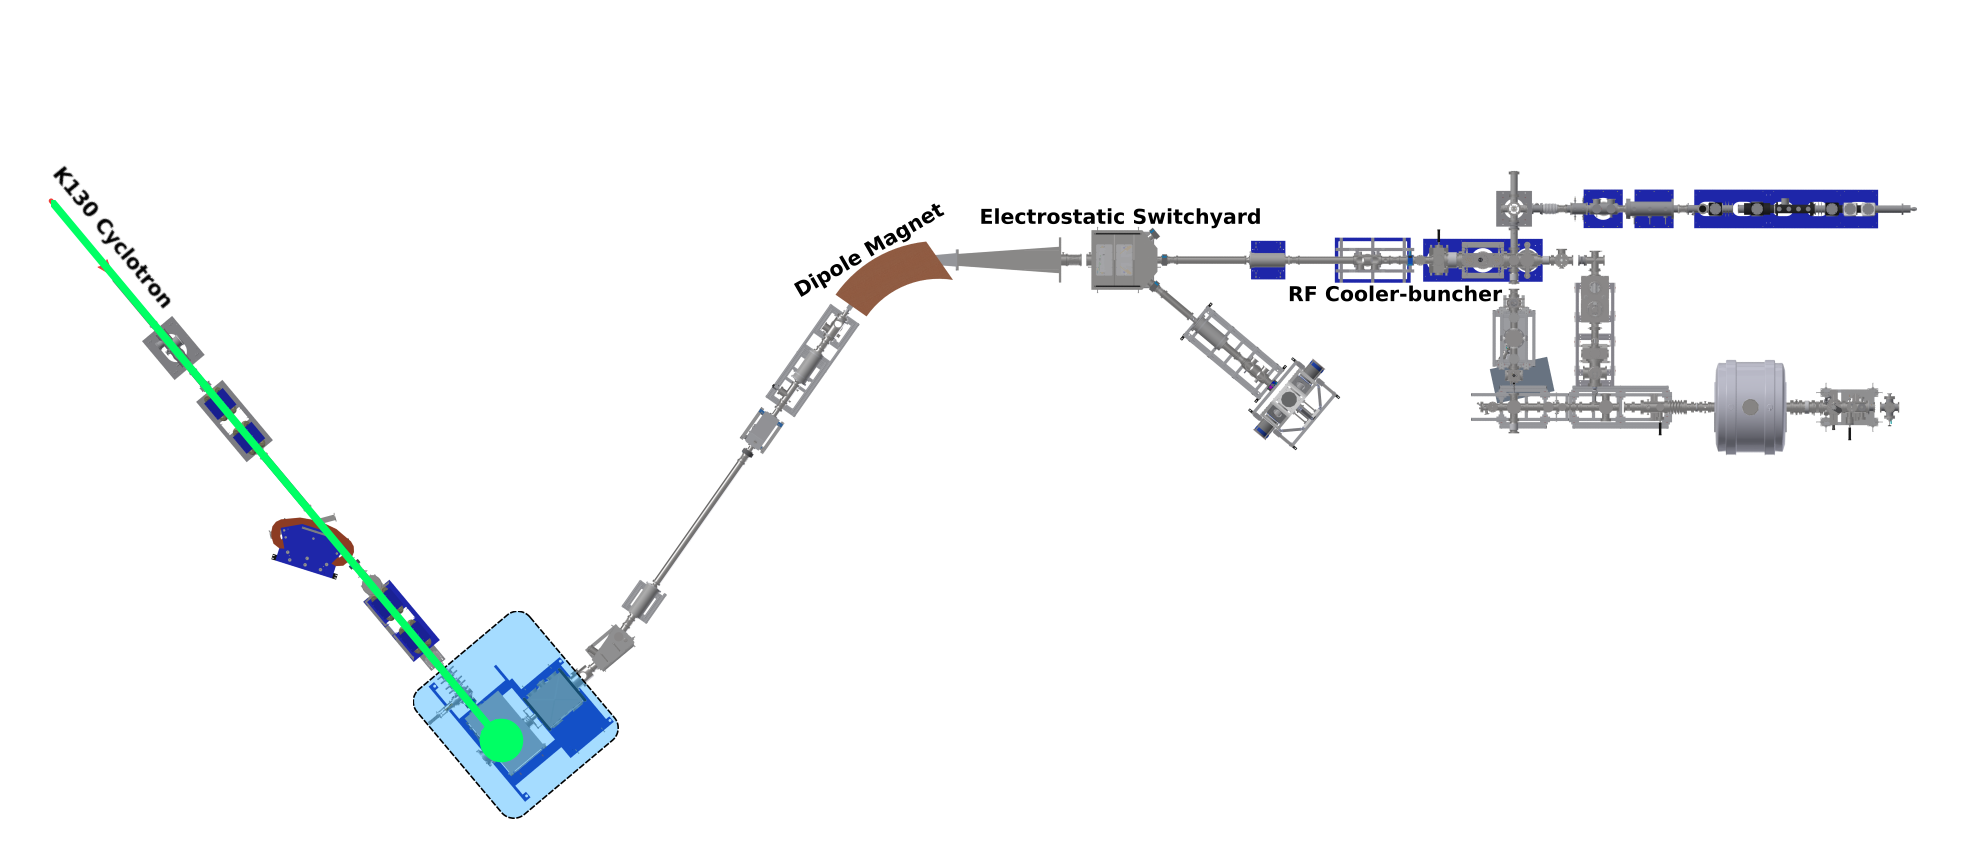
\includegraphics[width=\textwidth]{Igisol_scheme_TG_online.png}}%
		% \only<4>{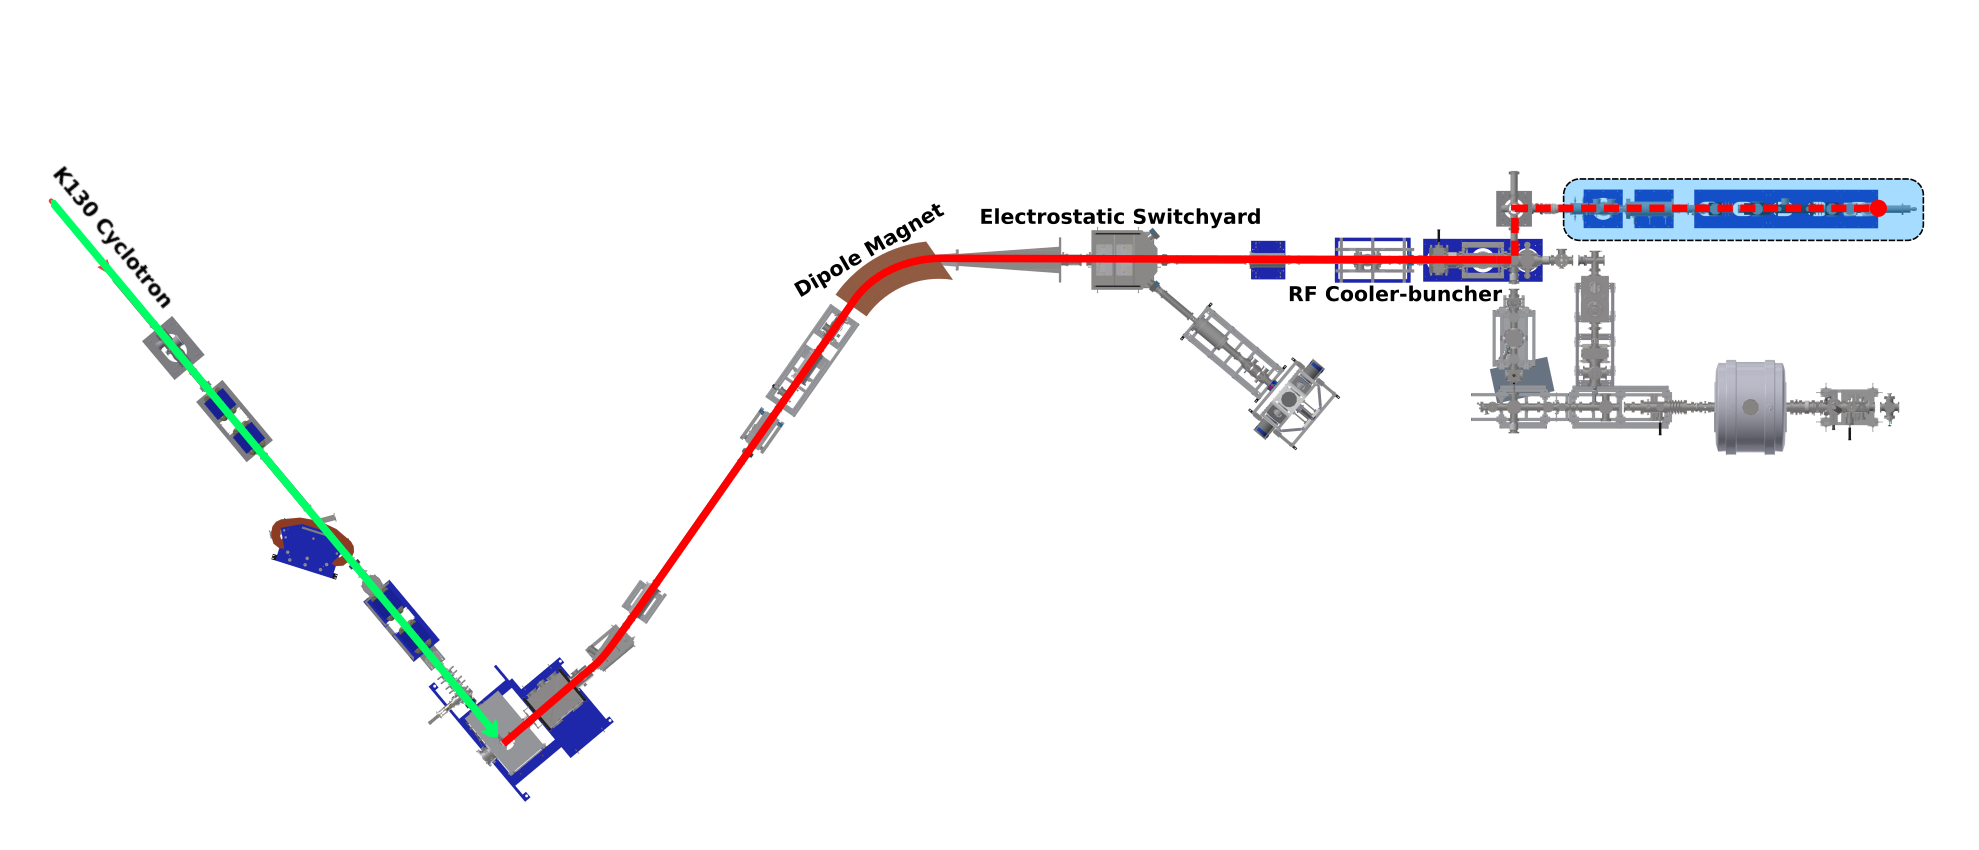
\includegraphics[width=\textwidth]{Igisol_scheme_CLS.png}}%
		% \only<5>{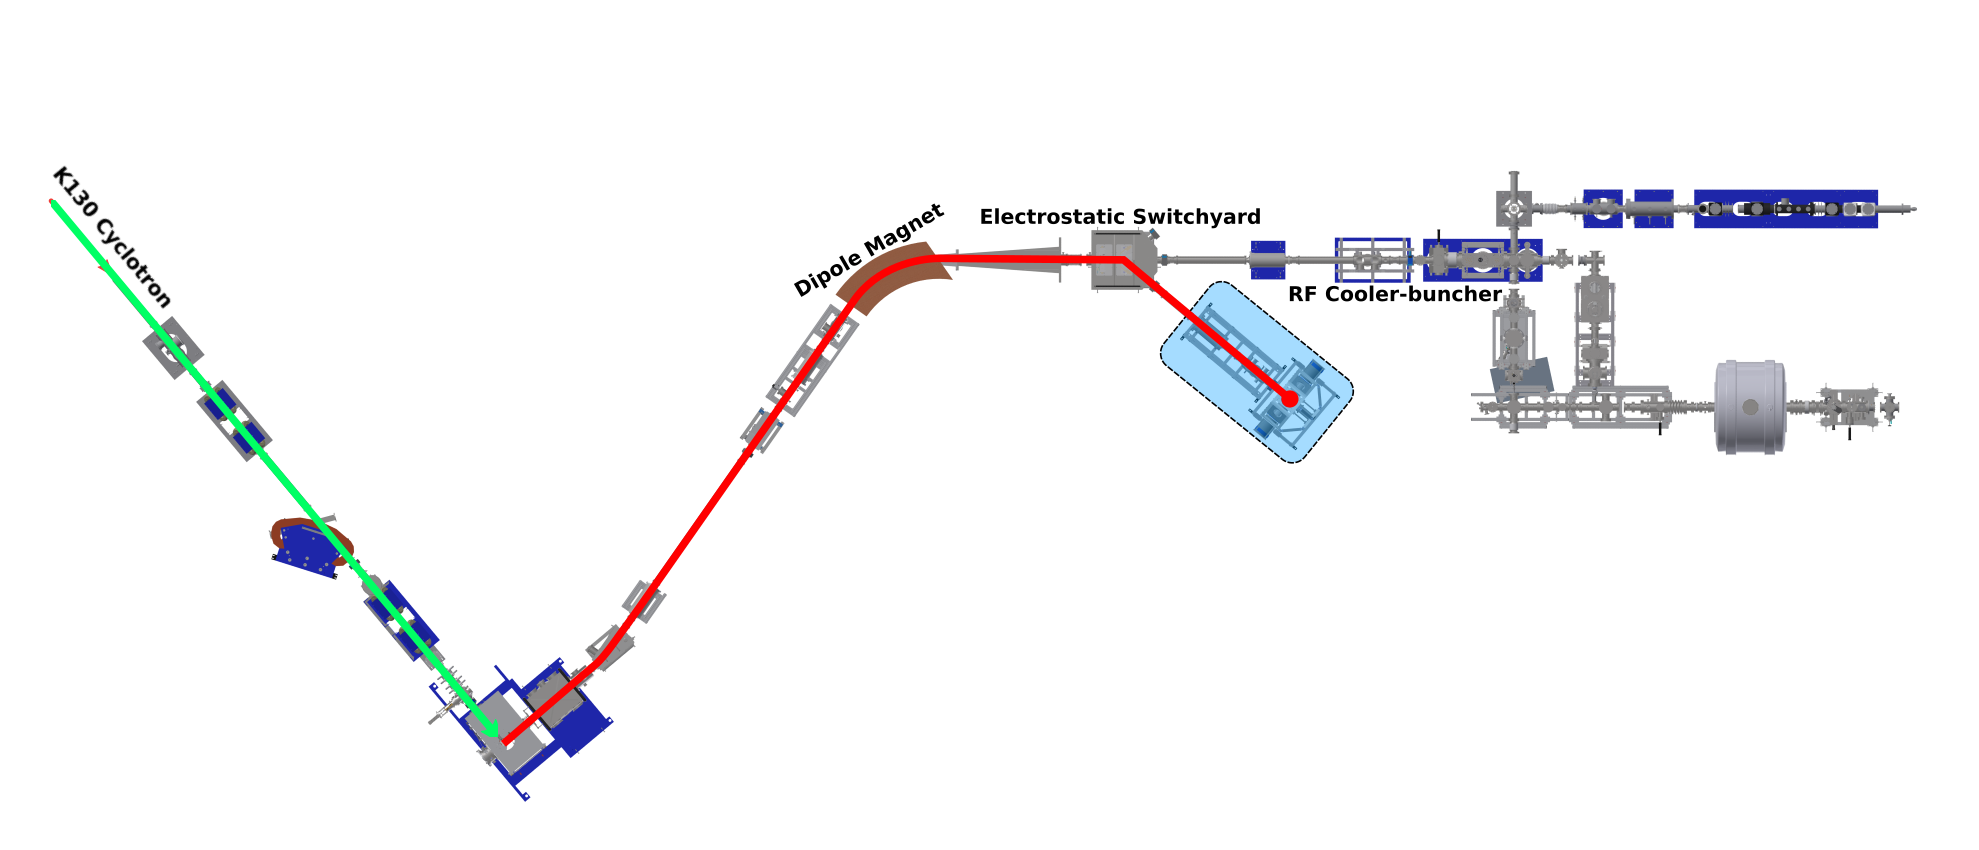
\includegraphics[width=\textwidth]{Igisol_scheme_Spec.png}}%
		% \only<6>{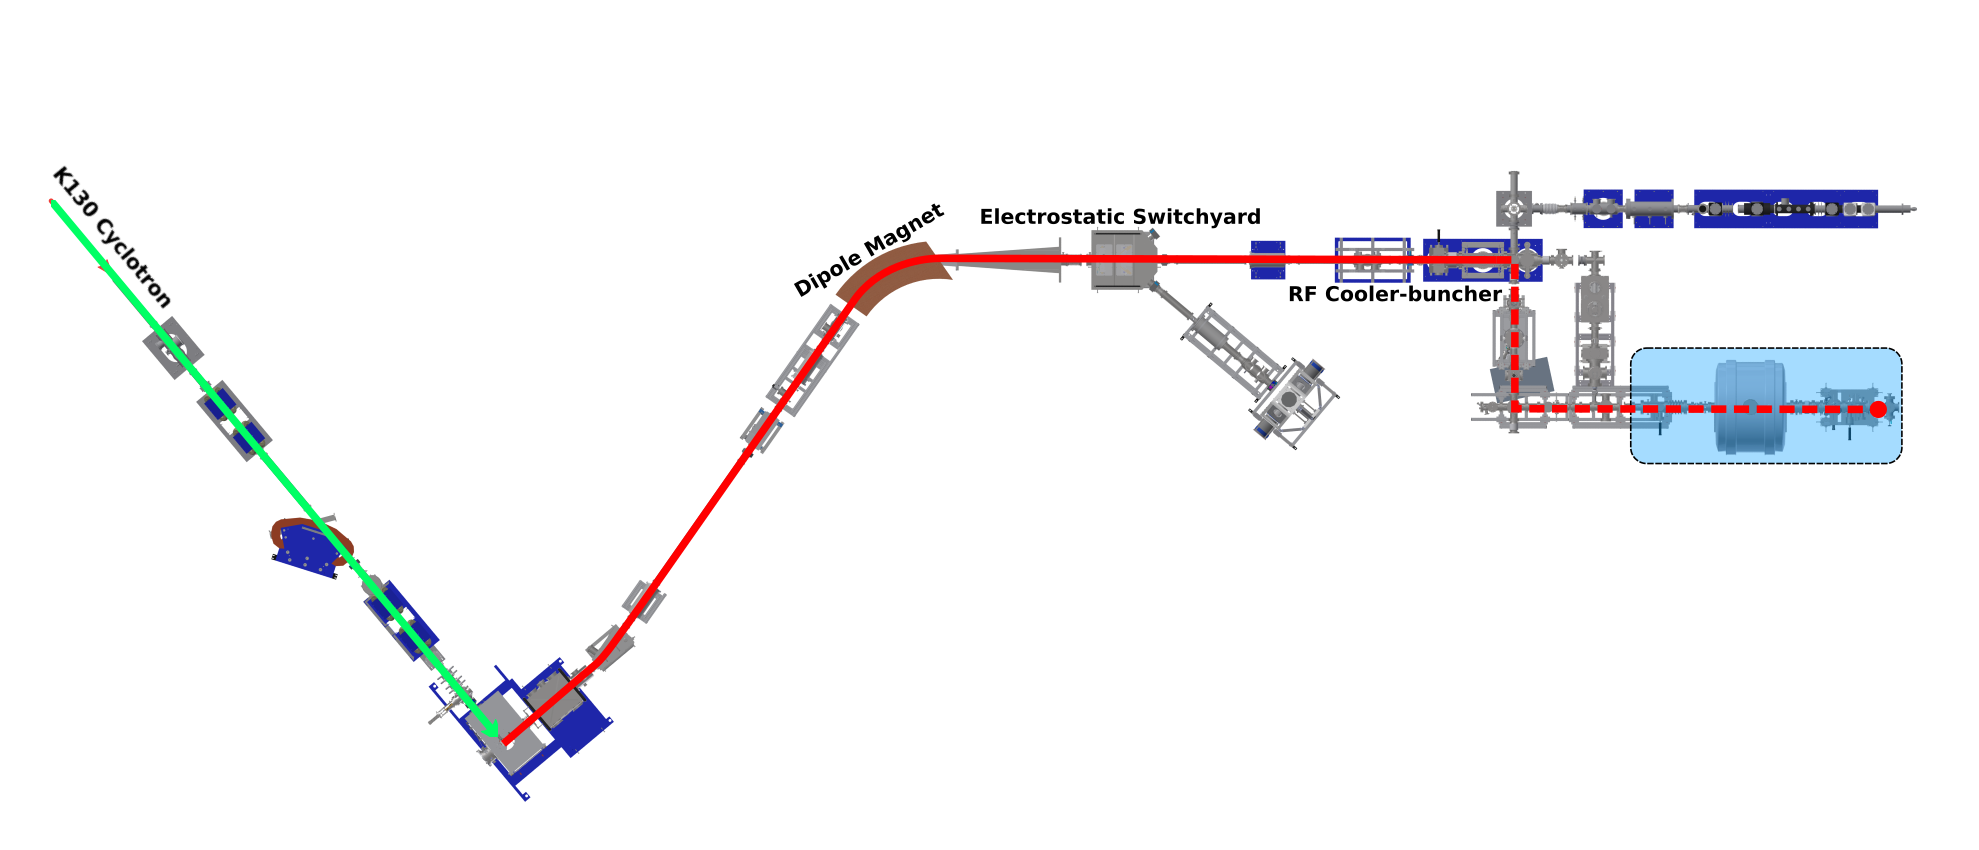
\includegraphics[width=\textwidth]{Igisol_scheme_Penn.png}}%
	\end{textblock*}
	\only<1>{
		\begin{textblock*}{0.13\paperwidth}(0.16\paperwidth,0.2\paperheight)
			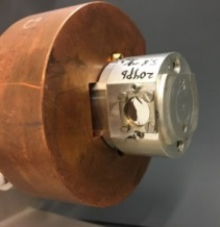
\includegraphics[width=0.8\textwidth]{LIONGUIDE.png}
		\end{textblock*}
		\begin{textblock*}{0.1\paperwidth}(0.82\paperwidth,0.2\paperheight)
			\only<1->{
\includegraphics[width=\textwidth]{jgu_logo_kasten.jpg}}%
		\end{textblock*}
		\begin{textblock*}{0.7\paperwidth}(0.32\paperwidth,0.45\paperheight)
			\textbf{Proton-Induced Fusion-evaporation reactions}
		\end{textblock*}

		\begin{textblock*}{0.5\paperwidth}(0.45\paperwidth,0.5\paperheight)
			\begin{itemize}
				\item Production of neutron deficient actinides
				\item Extraction times can be < 1ms 
			\end{itemize}
		\end{textblock*}
		\begin{textblock*}{0.15\paperwidth}(0.005\paperwidth,0.55\paperheight)
			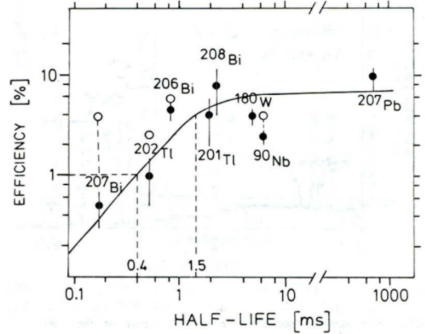
\includegraphics[width=\textwidth]{OldEfficiency.png}
		\end{textblock*}
		\begin{textblock*}{0.3\paperwidth}(0.16\paperwidth,0.49\paperheight)
			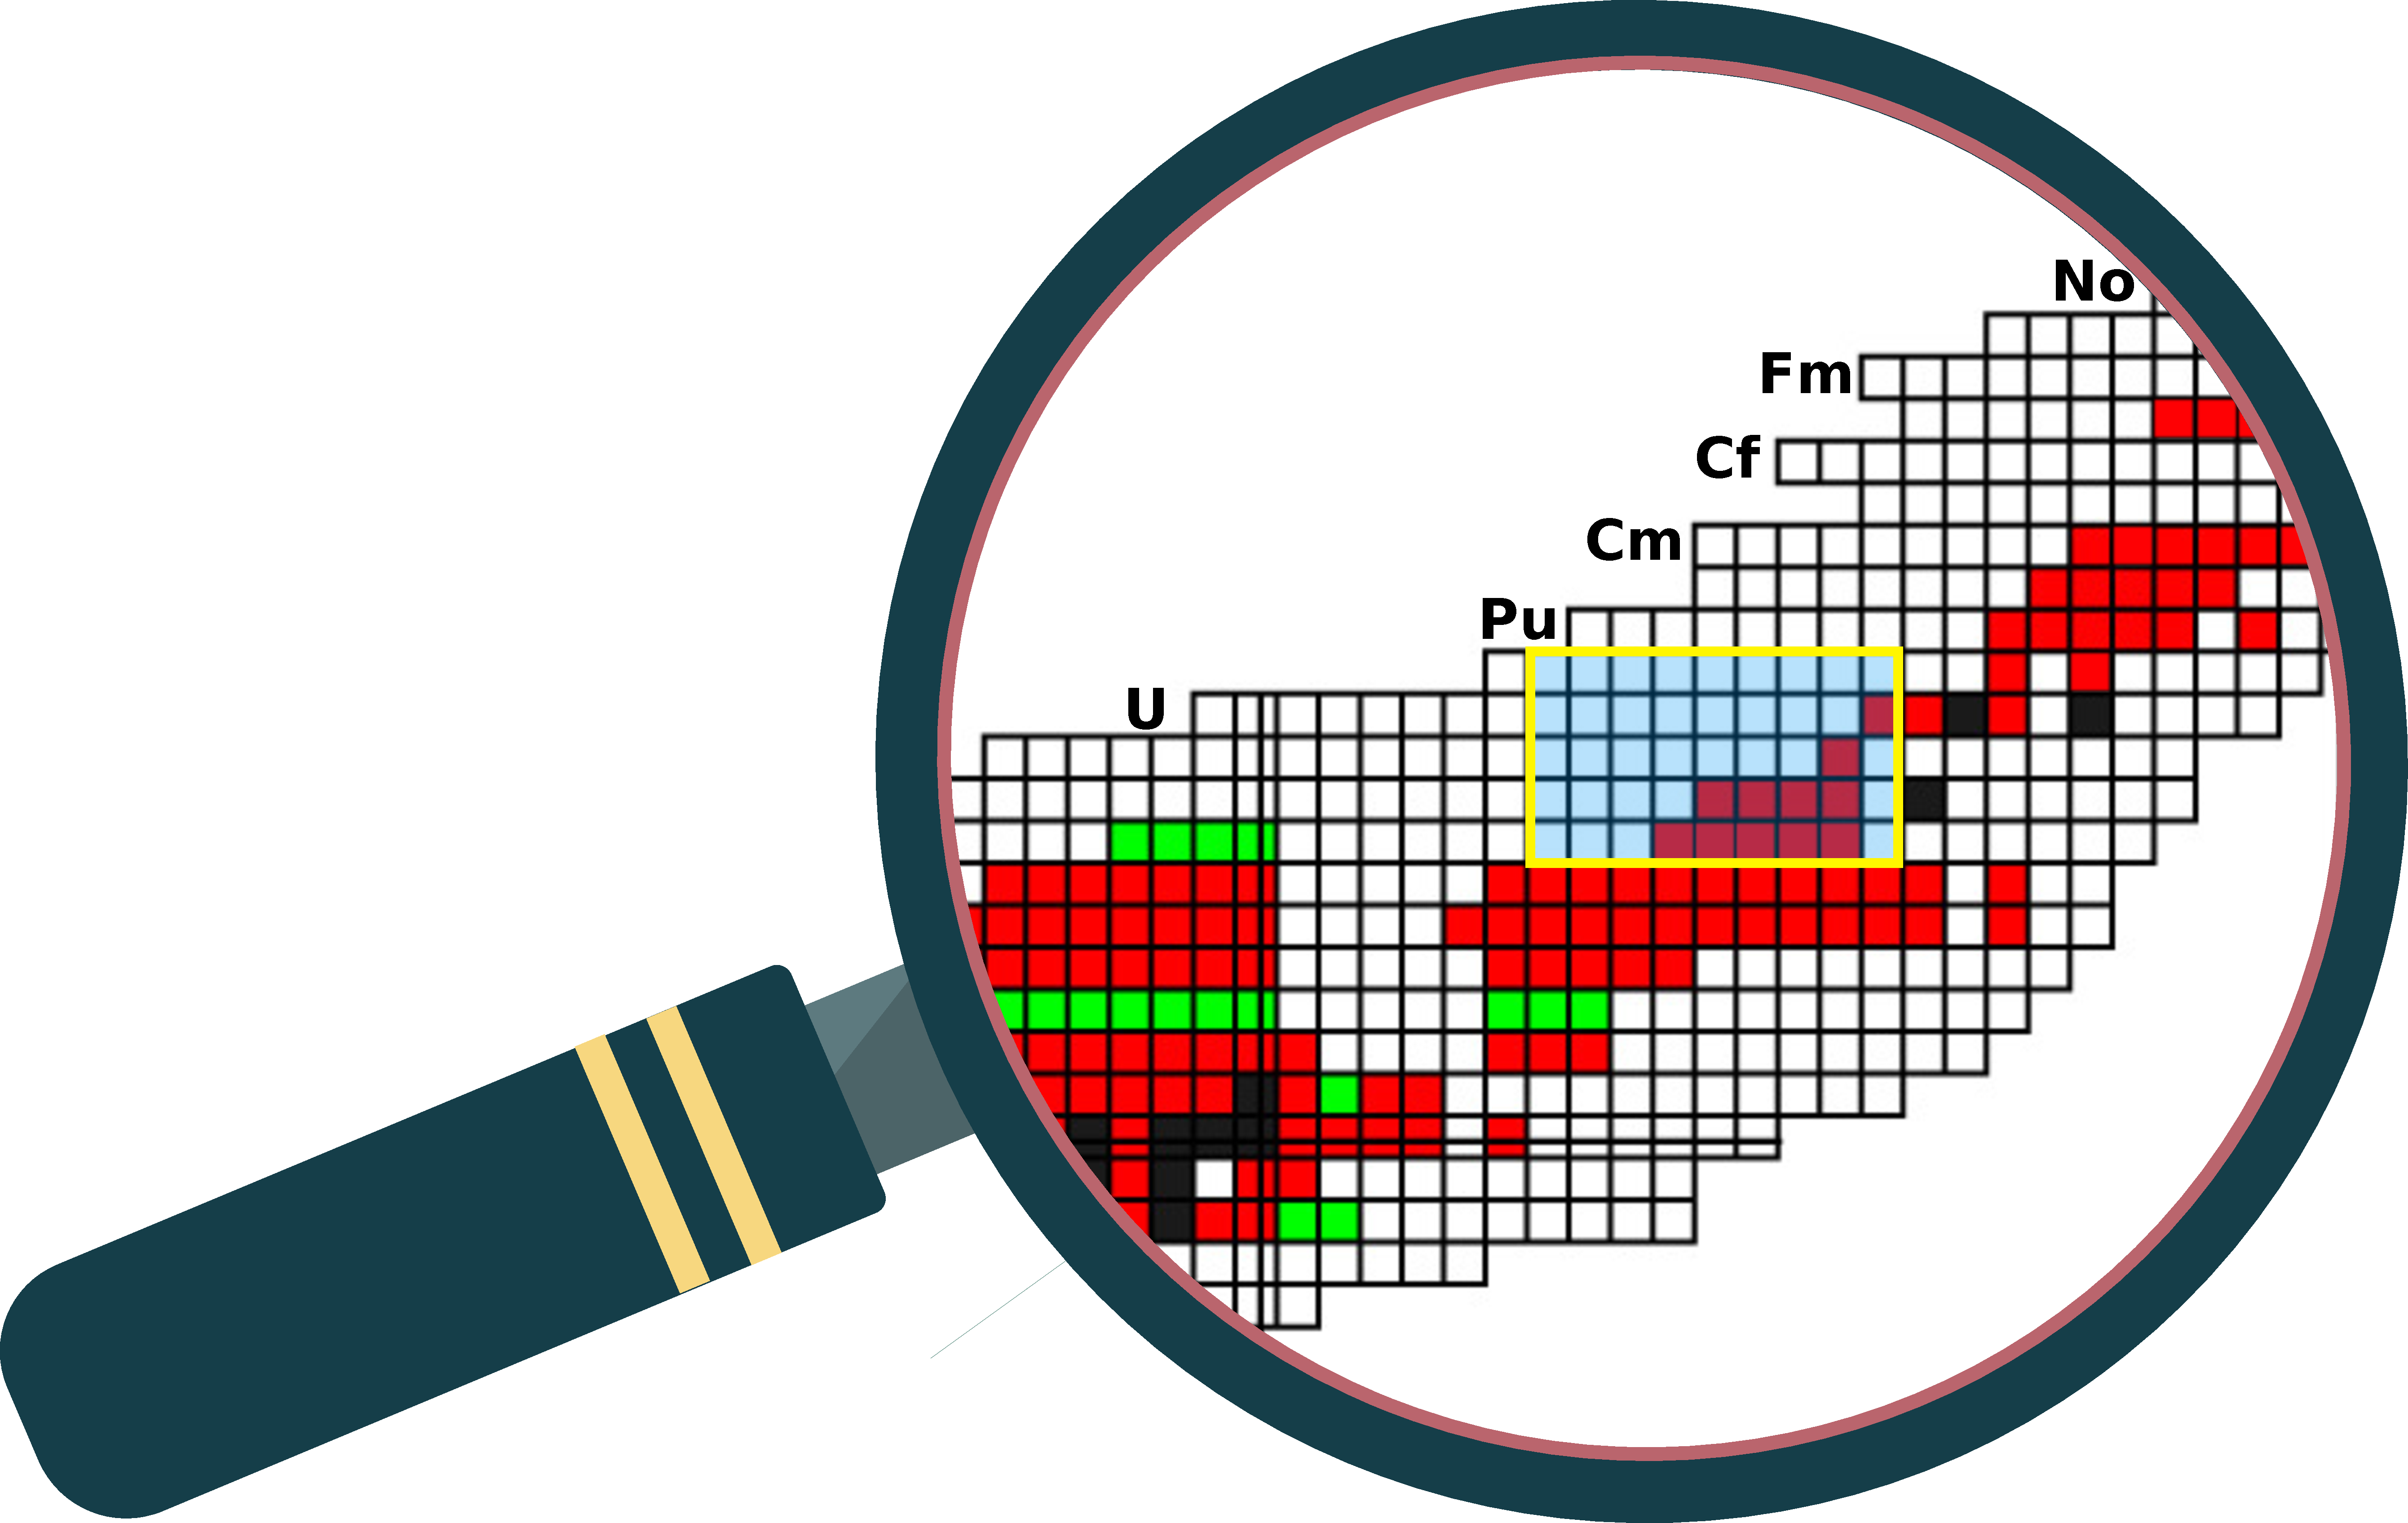
\includegraphics[width=\textwidth]{AChart_zoom.pdf}
		\end{textblock*}
		\begin{textblock*}{0.2\paperwidth}(0.47\paperwidth,0.64\paperheight)
			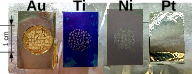
\includegraphics[width=\textwidth]{DODtarget.png}
		\end{textblock*}
		\begin{textblock*}{0.3\paperwidth}(0.68\paperwidth,0.64\paperheight)
			\textbf{DoD Target}
			\begin{itemize}
				\item Good target durability
				\item Production yield stability
			\end{itemize}
		\end{textblock*}
		\begin{textblock*}{0.1\paperwidth}(0.68\paperwidth,0.75\paperheight)
			\footnote{R. Haas et al., NIMA 874 (2017) 43}
		\end{textblock*}
		\begin{textblock*}{0.1\paperwidth}(0.01\paperwidth,0.75\paperheight)
			\footnote{J. Ärje, J. Äystö et al., Phys. Rev. Lett. 54 (1985) 99}
		\end{textblock*}
	}
	
\end{frame}


%----------------------------Fusion-evap---------------------------------
\begin{SectionTitle}
	\begin{frame}
		\centering
		\begin{textblock*}{0.9\paperwidth}(0.05\paperwidth,0.12\paperheight)
			\centering
			\textbf{\LARGE PROTON-INDUCED FUSION-EVAPORATION WITH ACTINIDE TARGET}	
		\end{textblock*}
		\begin{textblock*}{0.5\paperwidth}(0.25\paperwidth,0.4\paperheight)
			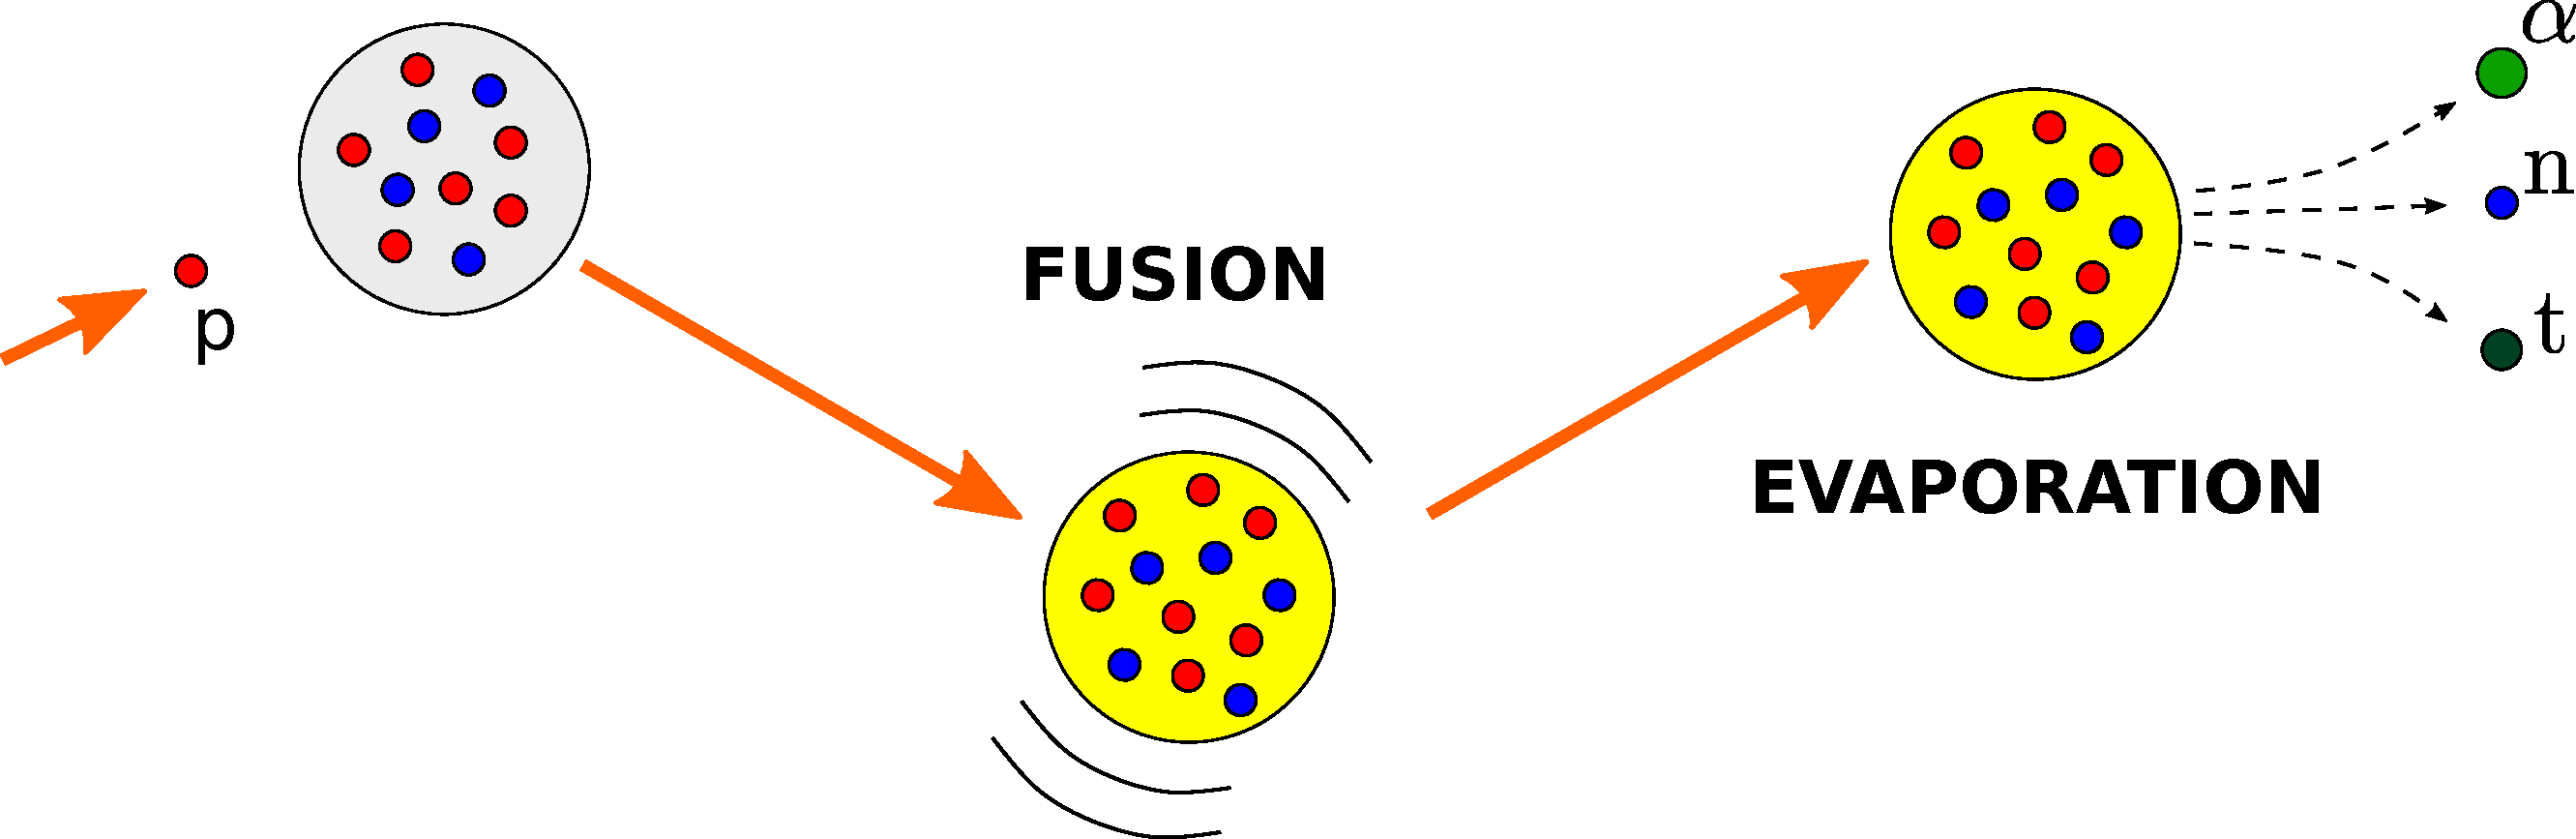
\includegraphics[width=.9\textwidth]{Reaction.pdf}
		\end{textblock*}
	\end{frame}
\end{SectionTitle}

\begin{frame}{Production yields}
	\begin{textblock*}{0.4\paperwidth}(0.05\paperwidth,0.2\paperheight)
		\only<1>{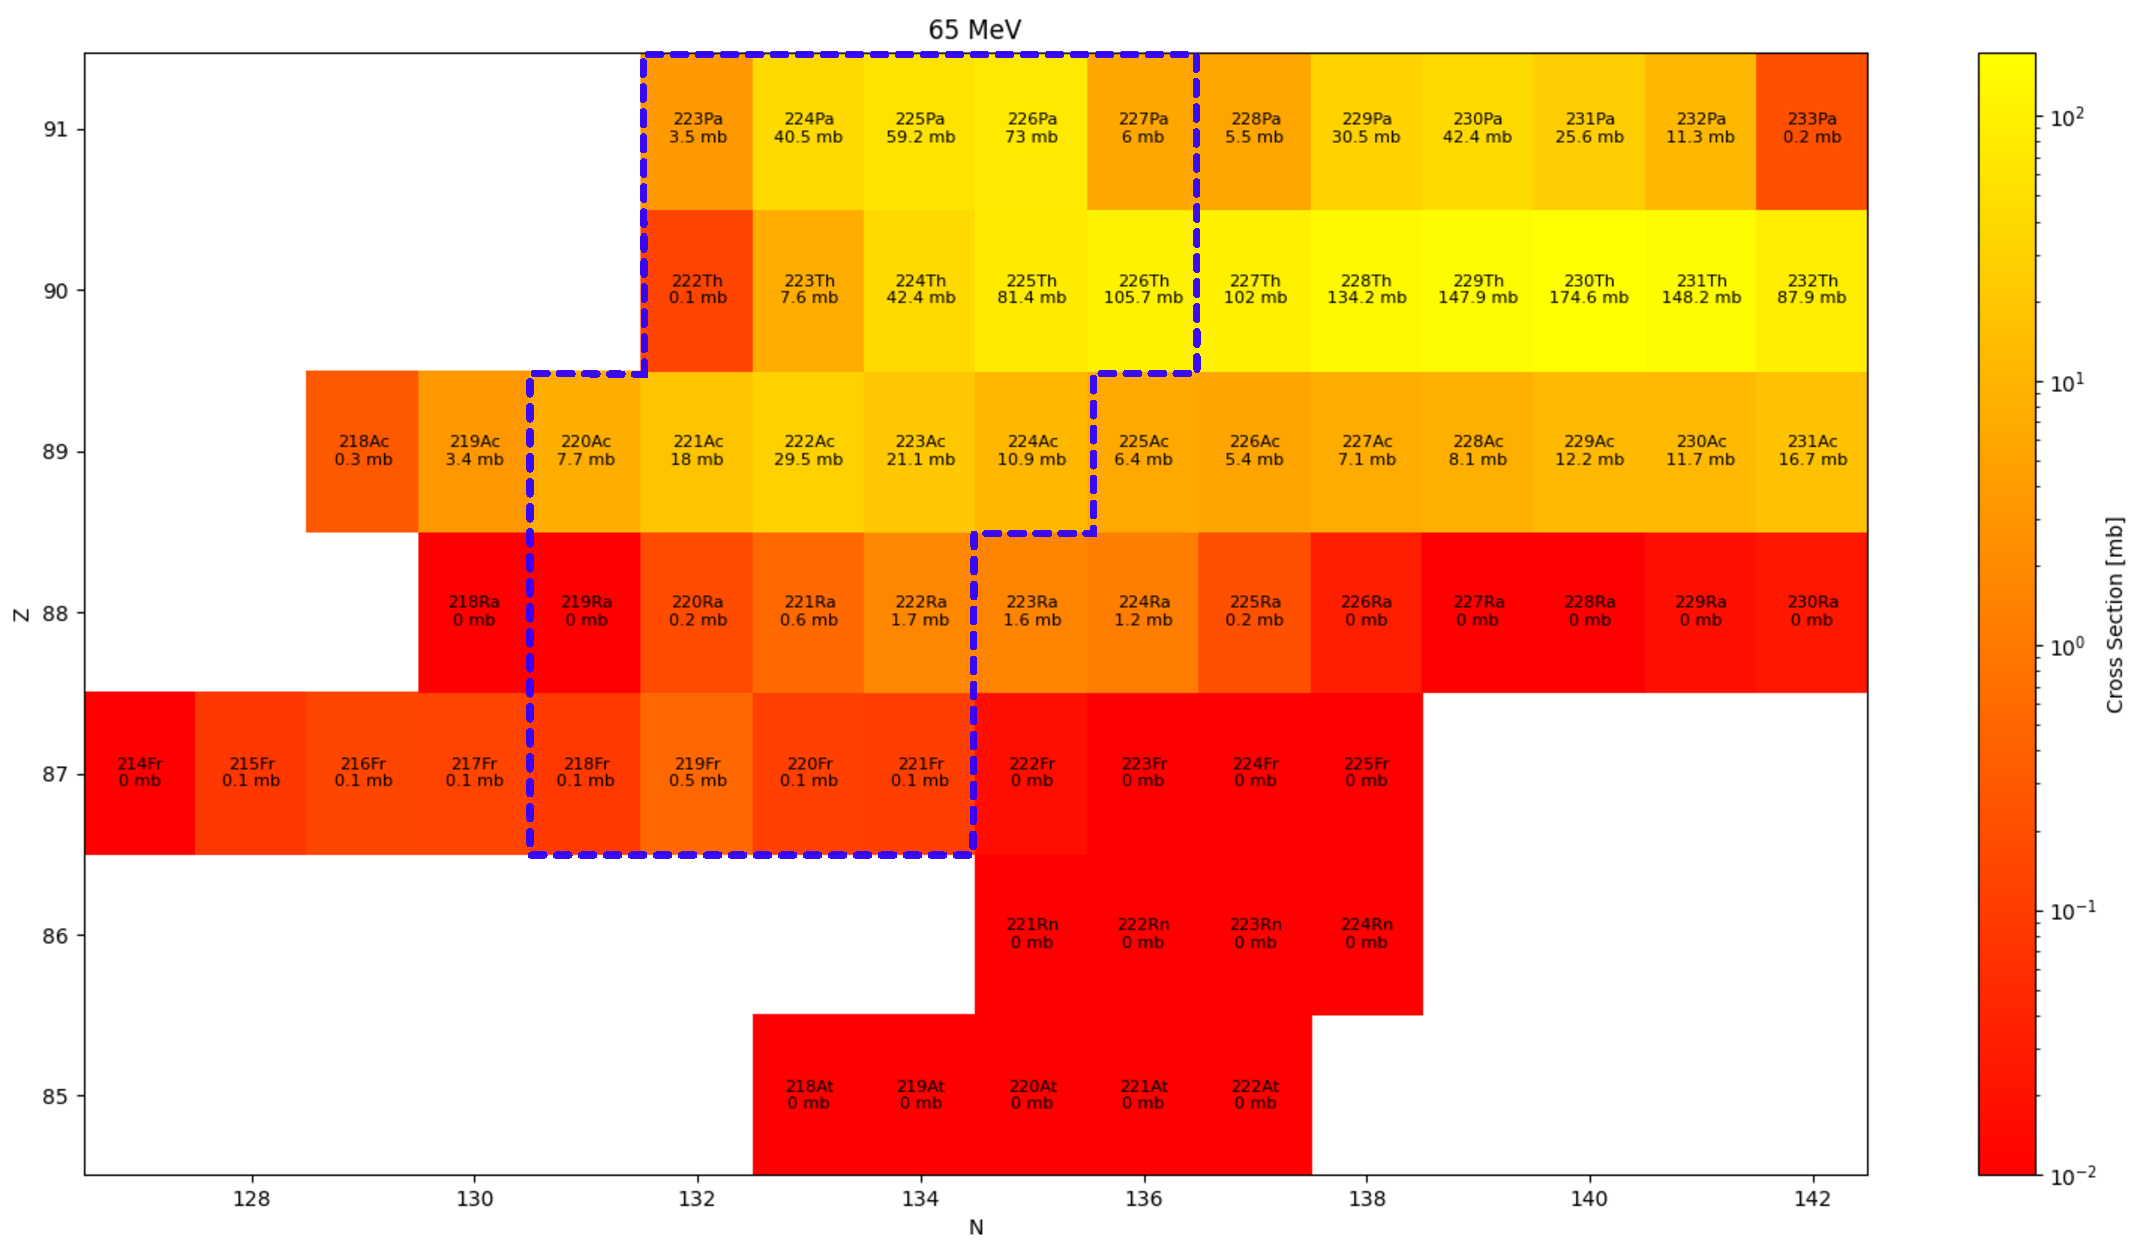
\includegraphics[width=\textwidth]{Production_CrossSections.pdf}}
		\only<2>{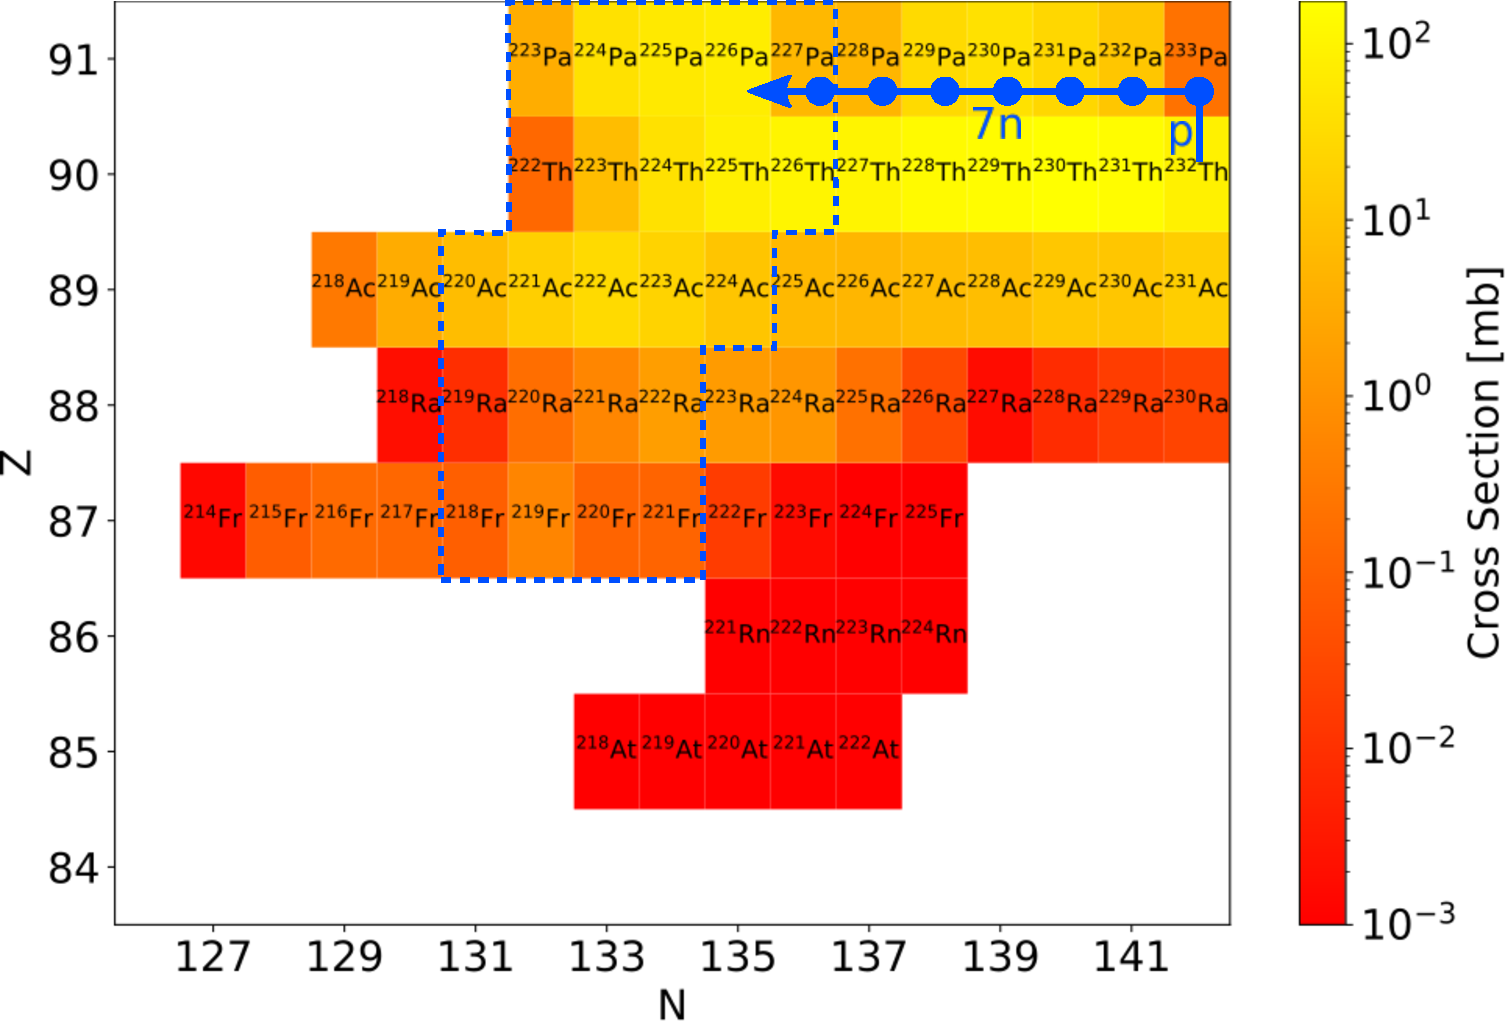
\includegraphics[width=\textwidth]{Production_CrossSections_tof.pdf}}
	\end{textblock*}
		\begin{textblock*}{0.6\paperwidth}(0.01\paperwidth,0.7\paperheight)
			\begin{itemize}
				\item<1-> Decay Spectroscopy experiment to evaluate yields?
				\item<2-> Detecting isotope with $\sim$1~ms<$\tau$<$\sim$3~h. 
				\item<2-> 65~MeV selected as optimal energy (8 nucleons evaporated)
			\end{itemize}
		\end{textblock*}
		\begin{textblock*}{0.45\paperwidth}(0.5\paperwidth,0.2\paperheight)
			\includegraphics[width=\textwidth]{simulationXS.pdf}
		\end{textblock*}
		\begin{textblock*}{0.5\paperwidth}(0.55\paperwidth,0.7\paperheight)
			\begin{itemize}
				\item Lack of experimental data
				\item Simulation routines gives different results
			\end{itemize}
			\qquad \qquad $^{232}$Th(p,pxn)Y
		\end{textblock*}

\end{frame}

\begin{frame}{Decay Spectroscopy}
	\begin{textblock*}{0.8\paperwidth}(0.01\paperwidth,0.1\paperheight)
		% \only<1->{\includegraphics[width=\textwidth]{Igisol_scheme_TG.png}}%
		% \only<1->{\includegraphics[width=\textwidth]{Igisol_scheme_TG_online.png}}%
		% \only<1>{\includegraphics[width=\textwidth]{Igisol_scheme_CLS.png}}%
		\only<1>{\includegraphics[width=\textwidth]{Igisol_scheme_Spec.png}}%
		% \only<6>{\includegraphics[width=\textwidth]{Igisol_scheme_Penn.png}}%
	\end{textblock*}
	\begin{textblock*}{0.2\paperwidth}(0.1\paperwidth,0.3\paperheight)
		\centering
		$^{232}$Th(p,X)Y\\65MeV
	\end{textblock*}
	\begin{textblock*}{0.2\paperwidth}(0.02\paperwidth,0.65\paperheight)
		\centering
		SELECTED ISOBARS\\
		A=218-227
	\end{textblock*}
	\begin{textblock*}{0.22\paperwidth}(0.28\paperwidth,0.48\paperheight)
		\includegraphics[width=\textwidth]{I262_Schematic_experiment_setup.pdf}
	\end{textblock*}
	\begin{textblock*}{0.4\paperwidth}(0.58\paperwidth,0.5\paperheight)
		\textbf{Experimental Setup}
		\small
		\begin{itemize}
			\item 4 BEGE detectors ($\gamma$)
			\item 2 Si quadrant detectors ($\alpha$)
			\item 1 Si(Li) detectors (e)
		\end{itemize}
		Resolve the decay scheme and lifetime of selected isotopes by $\alpha$-$\gamma$ coincidences
	\end{textblock*}
\end{frame}

\begin{frame}{226 Isobar chains}
	\begin{textblock*}{0.5\paperwidth}(0.01\paperwidth,0.2\paperheight)
		\only<1>{\includegraphics[width=\textwidth]{226Decay.pdf}}
		\only<2>{\includegraphics[width=\textwidth]{226Decay_pa.pdf}}
	\end{textblock*}
	\begin{textblock*}{0.55\paperwidth}(0.35\paperwidth,0.4\paperheight)
		\only<1>{\includegraphics[width=\textwidth]{AlphaVsGamma_226.pdf}}
		\only<2>{\includegraphics[width=\textwidth]{AlphaVsGamma_226_highlight.pdf}}
	\end{textblock*}

	\begin{textblock*}{0.3\paperwidth}(0.6\paperwidth,0.25\paperheight)
		\centering
		$\alpha$-$\gamma$ coincidence matrix\\
		2~$\mu$s time window
	\end{textblock*}
\end{frame}

\begin{frame}{$^{226}$Pa -preliminary- }
	\begin{textblock*}{0.4\paperwidth}(0.01\paperwidth,0.17\paperheight)
		\includegraphics[width=\textwidth]{Alpha_Gated.pdf}
	\end{textblock*}
	\begin{textblock*}{0.5\paperwidth}(0.4\paperwidth,0.23\paperheight)
		\only<1>{
		Current literature Q$_{\alpha}$ 6987(10)~keV \footnote{S. Singh, NDS 112 (2011) 2851}\\
		\includegraphics[width=\textwidth]{DecaySchemePa226.png}
		\vspace{-0.05\textheight}
		\begin{itemize}
			\item Preliminary analysis suggest the presence of a level $\sim$54~keV below the literature g.s.
		\end{itemize}}
		\only<2>{
			Current literature T$_{1/2}$ 1.8(2) min. \footnote{S. Singh, NDS 112 (2011) 2851}\\
			\includegraphics[width=0.6\textwidth]{Decay_time.pdf}\\
			\begin{textblock*}{0.3\paperwidth}(0.68\paperwidth,0.4\paperheight)
				\begin{itemize}
					\item $\alpha$ rate with beam pulser
					\item Gate on most intense $\gamma$ ray
					\item new half-life estimate:\\T$_{1/2}$ 1.58(7) min.
				\end{itemize}
			\end{textblock*}
		}
	\end{textblock*}
\end{frame}

\begin{frame}{Yields}
		\begin{textblock*}{0.5\paperwidth}(0.02\paperwidth,0.2\paperheight)
			\centering
			Increase in energy from preliminary experiment
			60~MeV$\rightarrow$65~MeV\\
			\vspace{0.04\textheight}
			\textbf{General yields increase}\\
			measured from known alpha decay rates
			\vspace{0.04\textheight}

			note: target alpha recoil or direct evaporation residual?\\
			\vspace{0.07\textheight}
			
			\textbf{Long lived isotopes production rate}\\
			$\downarrow$\\
			\textbf{Use of JYFL trap}\\	
		\end{textblock*}
		\begin{textblock*}{0.8\paperwidth}(0.5\paperwidth,0.2\paperheight)
			\small
			\begin{tabular}[5pt]{ l  c  c }
				Isotope &Yield [cps] 60MeV& Yield [cps] 65MeV\\
				\hline
				$^{226}$Pa&	157	    &460 \\
				$^{226}$Th&	96      &352 \\
				$^{225}$Pa&	15      &85 \\
				$^{225}$Th&	14      &73 \\
				$^{225}$Ac&	?       &? \\
				$^{224}$Pa&	-       &2 \\
				$^{224}$Th&	-       &7 \\
				$^{224}$Ac&	?       &120 \\
				$^{223}$Ac&	220     &400 \\
				$^{222}$Ac&	91      &148 \\
				$^{222}$Ra&	67      &144 \\
				$^{221}$Ac&	4       &20 \\
				$^{221}$Ra&	6       &7 \\
				$^{219}$Fr&	46      &55 \\
			\end{tabular}
		\end{textblock*}
\end{frame} 

\begin{frame}{\qquad JYFLTRAP - yield and mass measurements}
	\begin{textblock*}{0.3\paperwidth}(0.05\paperwidth,0.22\paperheight)
		\includegraphics[width=\textwidth]{JYFLTRAP.png}
	\end{textblock*}
	\begin{textblock*}{0.25\paperwidth}(0.7\paperwidth,0.3\paperheight)
		\includegraphics[width=\textwidth]{PIICR.png}\footnote{D.A. Nesterenko, EPJ. A 54 (2018) 154}
	\end{textblock*}
	\begin{textblock*}{0.3\paperwidth}(0.35\paperwidth,0.25\paperheight)
		\centering
		\textbf{PI-ICR technique}
		\begin{itemize}
			\item Yield of long lived isotopes
			\item Direct determination of Q$_{\alpha}$ values
			\item On-line production of $^{229}$Th
			\item Optimal beam energy?
		\end{itemize}
		\vspace{0.05\textheight}
		$\delta \nu (^{229}\text{Th},^{229}\text{Pa})\sim 0.7\ \text{Hz}$\\
		\vspace{0.0\textheight}
		1~s accumulation time\\ $\downarrow$\\ 0.05~Hz resolution		
	\end{textblock*}
\end{frame}

%----------------------------Fusion-evap---------------------------------
\begin{SectionTitle}
	\begin{frame}
		\centering
		\begin{textblock*}{0.9\paperwidth}(0.05\paperwidth,0.12\paperheight)
			\centering
			\textbf{\LARGE SUMMARY AND OUTLOOK}	
		\end{textblock*}
		\begin{textblock*}{0.5\paperwidth}(0.25\paperwidth,0.3\paperheight)
			\includegraphics[width=.5\textwidth]{Lens.pdf}
		\end{textblock*}
	\end{frame}
\end{SectionTitle}

\begin{frame}{Summary}
	\begin{textblock*}{0.4\paperwidth}(0.1\paperwidth,0.35\paperheight)
		\centering
		\begin{itemize}
					\item[]{Three production method tested\\
								\begin{itemize}
									\item Filaments
									\item $\alpha$ recoil sources
									\item Online production 
								\end{itemize}
							}
					\item[]{Interest in Actinide region\\
								\begin{itemize}
									\item Optical spectroscopy data
									\item Basic nuclear decay and structure information
								\end{itemize}							
					}
		\end{itemize}
	\end{textblock*}
	\begin{textblock*}{0.4\paperwidth}(0.5\paperwidth,0.25\paperheight)
		\centering
		\includegraphics[width=0.9\textwidth]{AChart_1.pdf}

	\end{textblock*}
\end{frame}

\begin{frame}{Outlook}
	\begin{textblock*}{0.4\paperwidth}(0.03\paperwidth,0.32\paperheight)
		\begin{itemize}
			\item[]<1->{LISA (\colorbox{yellow}{See B. Marsh talk})\\
						\begin{itemize}
							\item Production of $^{239}$Pu alpha recoil source
							 for $^{235}$U isomer production \\
						\end{itemize}}
			\vspace{0.02\textheight}
			\item[]<2->{Online production\\
					\begin{itemize}
						\item Approved experiment with $^{233}$U target
						\item $^{239}$Pu as Dod target?
					\end{itemize}
					}	
		\end{itemize}
	\end{textblock*}
	\begin{textblock*}{0.5\paperwidth}(0.47\paperwidth,0.2\paperheight)
		% \vspace{0.1\textheight}
		\only<1>{\includegraphics[width=0.7\textwidth]{LISA-logo.pdf}\\
				\hspace{0.3\textwidth}\includegraphics[width=0.4\textwidth]{U233SRC.png}}%
		\only<2>{\vspace{0.1\textheight}\includegraphics[width=0.7\textwidth]{AChart_zoom.pdf}}%
		
	\end{textblock*}
\end{frame}

\begin{frame} 
	\begin{textblock*}{0.98\paperwidth}(0.01\paperwidth,0.02\paperheight)
		\centering
		\includegraphics[width=0.96\textwidth]{JYU_closing.jpg}
	\end{textblock*}
\end{frame}


\end{document}

% https://www.uni-mainz.de/eng/108.php 
% https://www.studierendenwerk-mainz.de/en/essentrinken/universitaetscampus/mensa-georg-forster-gebaeude-gfg 
% https://play.google.com/store/apps/details?id=de.rki.coronawarnapp&hl=de&gl=US 